\documentclass{article}
\usepackage{graphicx}
\usepackage{minted}
\usepackage{float}
\usepackage{url}
\usepackage[table]{xcolor}
\usepackage[section]{placeins}

\usepackage{caption}
\usepackage{subcaption}


\usepackage[style=authoryear, backend=biber]{biblatex}
\addbibresource{references.bib}

\usepackage{titlesec}

% TODO REMOVE
% \setcounter{section}{+2}

\setcounter{secnumdepth}{4}

\titleformat{\paragraph}
{\normalfont\normalsize\bfseries}{\theparagraph}{1em}{}
\titlespacing*{\paragraph}
{0pt}{3.25ex plus 1ex minus .2ex}{1.5ex plus .2ex}

\title{Data Mining and Big Data Analytics Coursework}

\author{Student 4228665}
\date{December 2025}

\usepackage{geometry}
 \geometry{
 a4paper,
 total={170mm,257mm},
 left=20mm,
 top=20mm,
 }
 
\begin{document}
\begin{titlepage}
\centering
\vspace*{2cm}
{\LARGE\bfseries Implementation of a Network Security Device Using Raspberry Pi Firewall\par}
\vspace{2cm}
{\Large CSI\_5\_OSY Operating Systems\par}
\vspace{0.5cm}
{\Large Student ID: 4228665\par}
\vfill

\begin{center}
    
\includegraphics[]{lsbu-logo.jpg}
\end{center}

{\large Submission Date: 9th December 2025\par}
\end{titlepage}

\newpage
\begin{abstract}
\noindent
This report shows the development of building a network firewall using a Raspberry Pi single-board computer (SBC) and an external network interface card (NIC). Driven by the coursework brief and a strong understanding of industry technologies, DevOps practices, rising costs of commercial firewalls and the higher operational and financial cost of not having one. This coursework starts as implementing OPNsense but changes to Ubuntu's Iptables. The coursework focuses on establishing secure network segmentation using multiple firewall zones and policies to handle internal and external threats, addressing the project requirement for a dedicated network security device.
\end{abstract}

\newpage
\tableofcontents

\newpage
\listoffigures

\newpage
\section{Introduction}
\label{sec:intro}

Network security has always been a warranted topic of concern in computer networks. A way to prevent or mitigate some of that concern on a network is to implement a firewall. Firewalls are able to prevent the spread of unwanted or malicious programs or data across networks/zones \parencite{blansit2009} and reduce the damage of a compromised network. While enterprise-level firewalls can cost upwards of \$40,000 USD \parencite{blueskysystems2025}, a local/home firewall can be made inexpensive using a Raspberry PI single-board computer (SBC) and open source software for significantly less \parencite{thepihut2025} \parencite{opnsense2025}. This project implements a lightweight firewall solution using a Raspberry Pi, turning the SBC into a dedicated network security device with multiple firewall zones and policies to ensure network traffic traverses the network as per the example in figure \ref{fig:basic-fw-diagram}. This will ensure proper packet filtering and traffic management on the network the firewall is used on.

\begin{figure}[H]
    \centering
    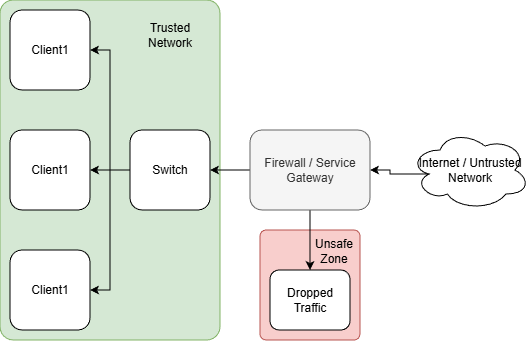
\includegraphics[width=0.6\linewidth]{Diagrams/os-fw-diagram.drawio.png}
    \caption{A diagram showcasing basic firewall filtering. showing how incoming traffic comes from the internet or an untrusted network, connects to the Firewall / Service gateway and is either passed to the LAN or dropped.}
    \label{fig:basic-fw-diagram}
\end{figure}

At its core, the coursework task put out is to install and configure a firewall application on a Raspberry Pi to act as a standalone firewall, as previously mentioned, while showing adequate knowledge and understanding of networking protocols (via traffic control, packet filtering, routing) and other approaches with self-hosting network devices, such as network monitoring and general observability \parencite{opencloudification2025} \parencite{dadiyala2023}. By using the Pi's onboard hardware and an additional network interface card (NIC), you can secure a home or small-to-medium-sized office network when paired with a Linux-based operating system like OPNsense \parencite{opnsense2025} (an open-source firewall and routing platform). OPNsense resembles a VM-based option for a service gateway (similar to Juniper's offering on its SRX line of hardware) that can provide routing, multi-WAN support, and VPNs, as well as firewall-specific features like network filtering, rule-based forwarding, and traffic (deep packet) inspection. What makes it more than just a firewall (a service gateway) is that it operates at all layers of the OSI model, not just layers 1-4. This project creates a general network service gateway capable of managing traffic between three distinct network interfaces, each representing different security zones.

\begin{figure}[H]
    \centering
    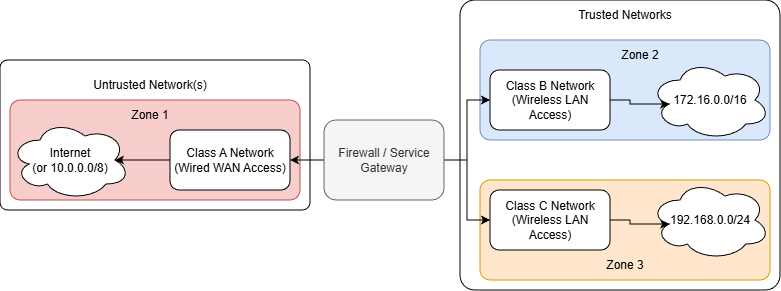
\includegraphics[width=0.8\linewidth]{Diagrams/os-fw-implementation-diagram.drawio.png}
    \caption{A diagram showing the different network ranges, the interfaces (and types) they're connected to and how they'll be isolated and sat within different firewall zones.}
    \label{fig:basic-fw-breakdown}
\end{figure}

TO EXPLAIN DIFFERENCES BETWEEN CLASSFUL NETWORK DECLARATIONS

This task calls for building a multi-interface firewall supporting Class-A, Class-B, and Class-C networks (as highlighted in Figure \ref{fig:basic-fw-breakdown}), and implementing firewall policies including default-deny rules and essential service permissions (allowing DNS, DHCP, and ICMP traffic) between the zones. Moreover, the work should allow internal/management network communication (to access the firewall), network address translation for internet access, and some form of logging for analysis and troubleshooting. Furthermore, the project calls for performance monitoring and evaluation to assess the system’s scalability and effectiveness under various traffic conditions outlined in the brief.
\section{Domain of Knowledge}
\label{sec:domain}

\subsection{What is a Firewall?}
\label{subsec:firewall-fundamentals}

A firewall is a network security device (or virtual application) that monitors and controls traffic based on rules and policies defined by an administrator \parencite{cisco2024firewall}. As shown in figure \ref{fig:basic-fw-diagram}, firewalls typically sit on the network edge, between the local network and a wider WAN (in this case, the internet via the class A interface) to filter / outright block untrusted traffic. Despite sitting on the edge of a network, firewalls also filter and allow/block traffic internally (on the LAN side) for trusted communication between networks (as shown in the ranges in Figure \ref{fig:basic-fw-breakdown}).

Firewalls are mainly used in networks for packet filtering, which requires inspecting IP packets and checking headers of the packets to determine their legitimacy against pre-defined firewall policies and rules \parencite{paloalto2025packet}. A firewall policy (or rule) is a declarative line of code that specifies whether a packet can traverse across the firewall or not, depending on specific attributes. For instance if a ubuntu server were only to allow incoming ssh connections and not telnet (as it is insecure and unencrypted), you would configure a UFW (Ubuntu's 'Uncomplicated Firewall') policy that either allows (whitelisting) only traffic on port 22 (SSH default port) or one that disallows (blacklisting) port 23 for both IPv4 and IPv6. This policy is shown in figure \ref{fig:UFW-example}. Firewalls also filter based on other attributes of packets, across the OSI model, taking into account the source and destination of a packet and the protocol of the packet, all of which can determine whether a packet is allowed, dropped, or denied by a firewall.

\begin{figure}[H]
    \centering
    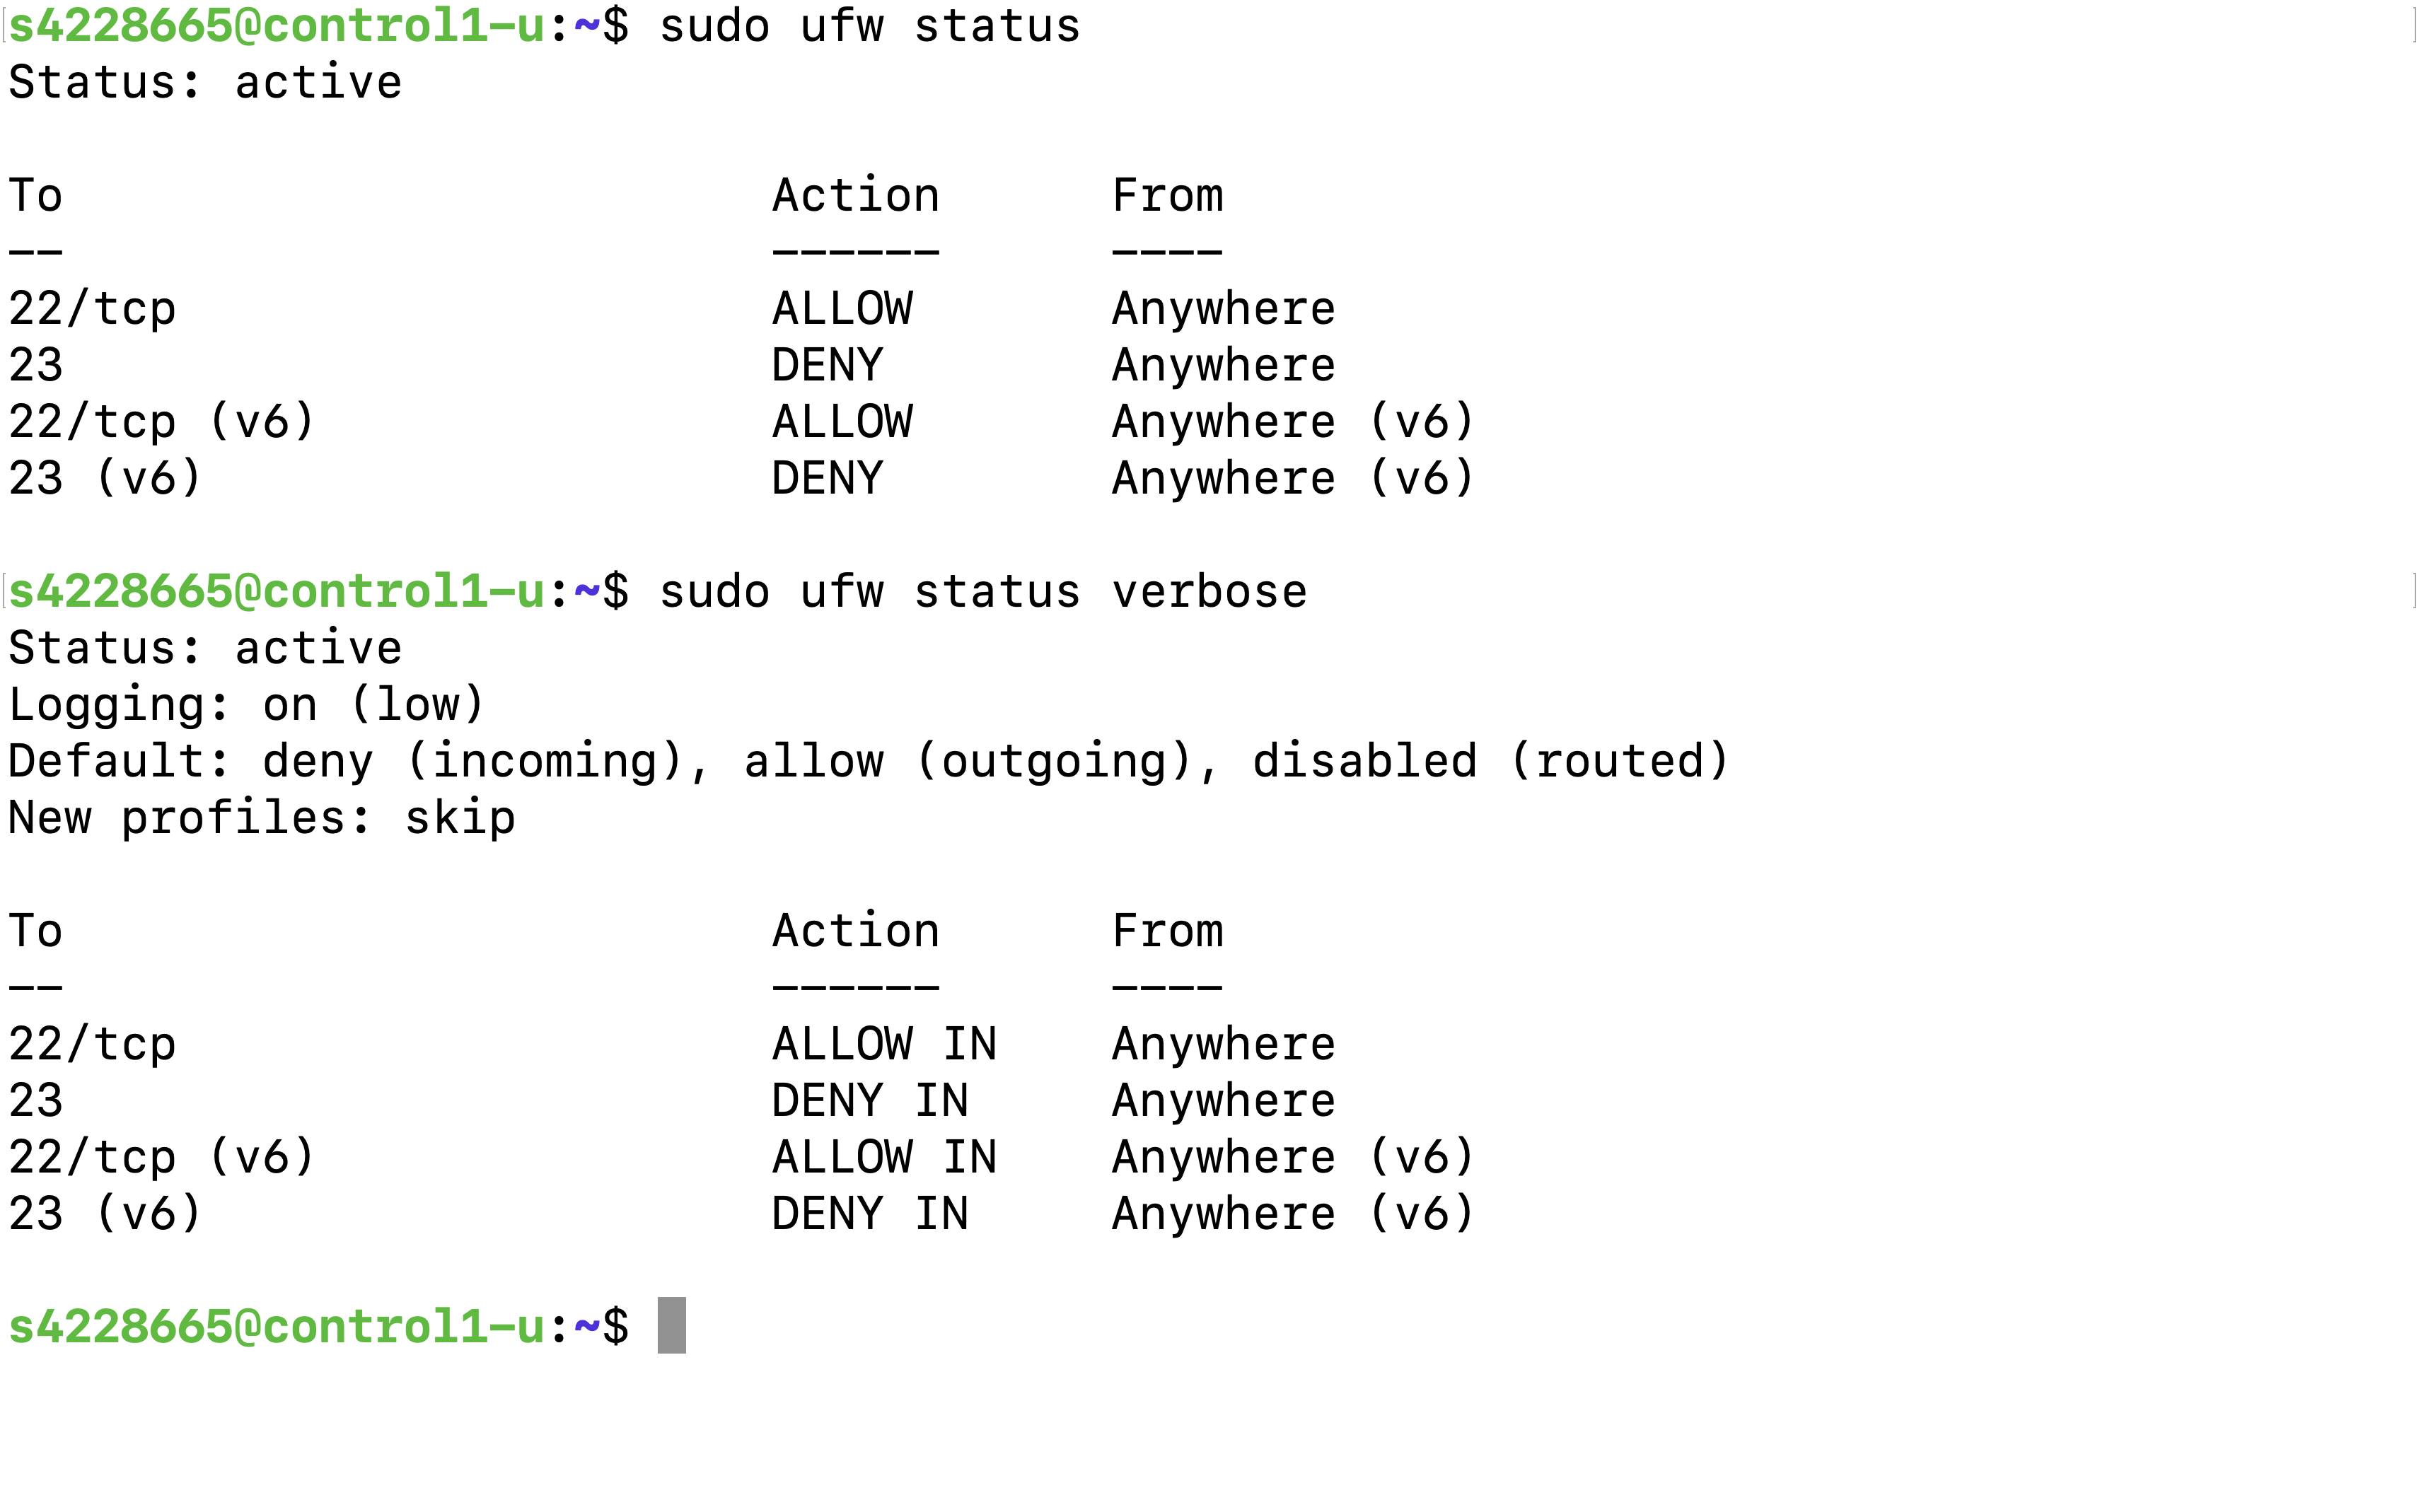
\includegraphics[width=0.8\linewidth]{Report_Images/os-ufw-screenshot.png}
    \caption{A screenshot from a Raspberry Pi running Ubuntu showcasing UFW policies to block port 23 (Telnet) and allow port 22 (SSH) connections. The verbose output shows the default rules of allowing all outgoing traffic but disabling default traffic going to the host.}
    \label{fig:UFW-example}
\end{figure}

To further secure a network, designers often segment it into different zones \parencite{paloalto2025privilege}, each with its own trust levels but still isolated from the others via firewall policies that allow only necessary traffic between networks. The coursework task also calls for this via an external Class-A network representing the untrusted internet connection, and two internal networks (Class-B and Class-C) simulating different frequency bands with different security requirements.

Following the "Never trust, always verify" approach \parencite{ravi2025beyond} to network security, firewalls should follow the principle of least privilege (PoLP) \parencite{paloalto2025segmentation}. PoLP works by limiting the amount of accessible data, resources, and applications to hosts/roles explicitly allowed to access them. Figure \ref{fig:UFW-example} does this by explicitly allowing only SSH connections instead of working and allowing SFTP (as an example) connections, which would be allowed if there were no firewall in place. This approach minimises the potential attack surface on the network and ensures that only necessary communications are allowed.

\subsection{Firewall OS Integration}
\label{subsec:os-integration}
To install an operating system on a typical (x86-based CPU) pc, you would create a boot medium. This can be done by installing the OS' image (.iso) file then running it through software that would take the .iso file and create a bootable usb-drive (or disk) that when inserted into the PC (and a user navigates to the boot options of the BIOS/UEFI) will boot to the install medium so a user can configure the OS install. This is how OPNsense would be installed on a supported x86 system. Unlike traditional x86-based hardware (in this case a firewall OS/distribution) that require installation to a storage medium, ARM-based systems like the Raspberry Pi require a different process. Instead of mounting the ISO image for installation, the Raspberry Pi requires a firmware image to be directly written (or "flashed") to the SD card, which serves as both the boot medium and primary (main) storage component

In discovering this, it was important to change plans to pick an implementation that would support the ARM-based CPU that the Raspberry Pi supports, as OPNsense only supports x86 CPUs. Another implementation of a network firewall is Ubuntu 24.04 with Iptables, an administration tool for IPv4 packet filtering and NAT \parencite{skilluped2020iptables}. This approach allows for a deeper understanding of Linux's netfilter kernel module and allows modern DevOps Infrastructure as Code practices (instead of using Opnsense's API) to be further explored in section \ref{sec:IaC}.

Ubuntu's netfilter framework, accessed through iptables, includes stateful packet inspection, network address translation (NAT), connection tracking, and logging \parencite{GeeksforGeeks2025iptables}. The system can be configured as a dedicated network gateway by enabling IP forwarding, configuring the three network interfaces (one USB-to-Ethernet adapter for the Class-A WAN interface, the built-in Ethernet for Class-B, and the onboard WiFi for Class-C as per figure \ref{fig:basic-fw-breakdown}), and implementing the required firewall changes through Iptables' rules. This approach aligns with professional practices where many enterprise firewalls are essentially hardened Linux systems running thier own implementation of Netfilter with custom software \parencite{IPv6Hawaii2024FirewallPerformance} like OpenWRT, the open source routing/firewall system \parencite{OpenWrt2024Official}.

\subsection{What is Iptables?}
Iptables is a command-line utility for configuring the packet filtering firewall in the Linux kernel's Netfilter framework \parencite{Linux2024IptablesManual}. The packet filtering is broken down into 3 different structures:
\begin{itemize}
    \item Tables \\
    This is the main mechanism behind iptables, as this is what is used to make decisions about whether a packet should be allowed to traverse the firewall, the main table of this implementation will be the filter table (there are also mangle, nat and raw tables that serve other features related to altering packet headers, routing based on NAT and even working with packets before hitting the kernel reads it) \parencite{BooleanWorld2024IptablesGuide}.
    \item Chains \\
    Tables are composed of different chains that do the packet filtering at various points of transmission though the firewall. Iptables has several chains but the ones used for this implementation are Input, Forward and Output, all associated with the filter table. Figure \ref{fig:iptables_breakdown} shows the chains and what tables they work with.
    \item Targets \\
    As the name suggests, targets determines where a packet ends up, if it's allowed though the firewall to a specific zone or if it's terminated and dropped from transmission depending on the rules/policies used.\parencite{DigitalOcean2024IptablesTutorial}
\end{itemize}

\begin{figure}[H]
    \centering
    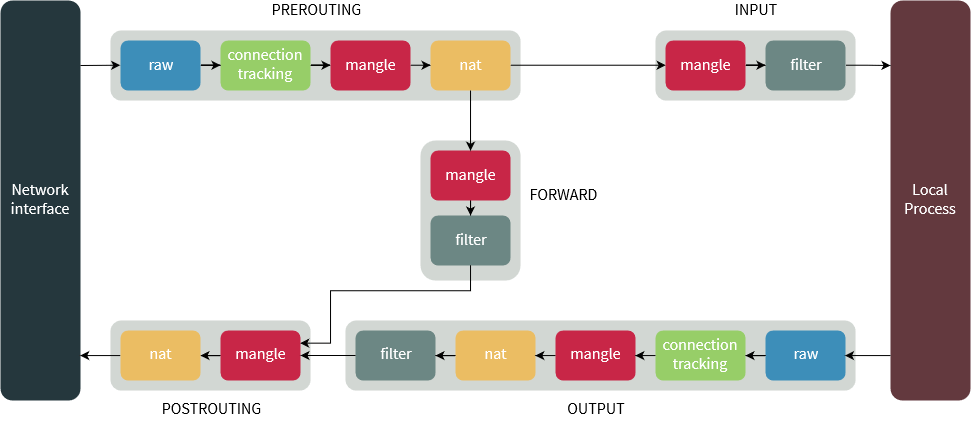
\includegraphics[width=0.8\textwidth]{Diagrams/os-iptables-chains.png}
    \caption{Iptables' chains and tables overview}
    \label{fig:iptables_breakdown}
    \parencite{BooleanWorld2024IptablesGuide}
\end{figure}

Using the same Raspberry Pi as seen in figure \ref{fig:UFW-example}, we can create another firewalling example of blocking icmp traffic using a simple iptables rule using the  example of An example of an iptables rule to block icmp traffic to a host using the \verb|input| table. First we can validate that icmp packets can hit the host, to test this we can ping the Raspberry Pi (figure \ref{example:iptables-ping-before}).


\begin{figure}[H]
  \centering
  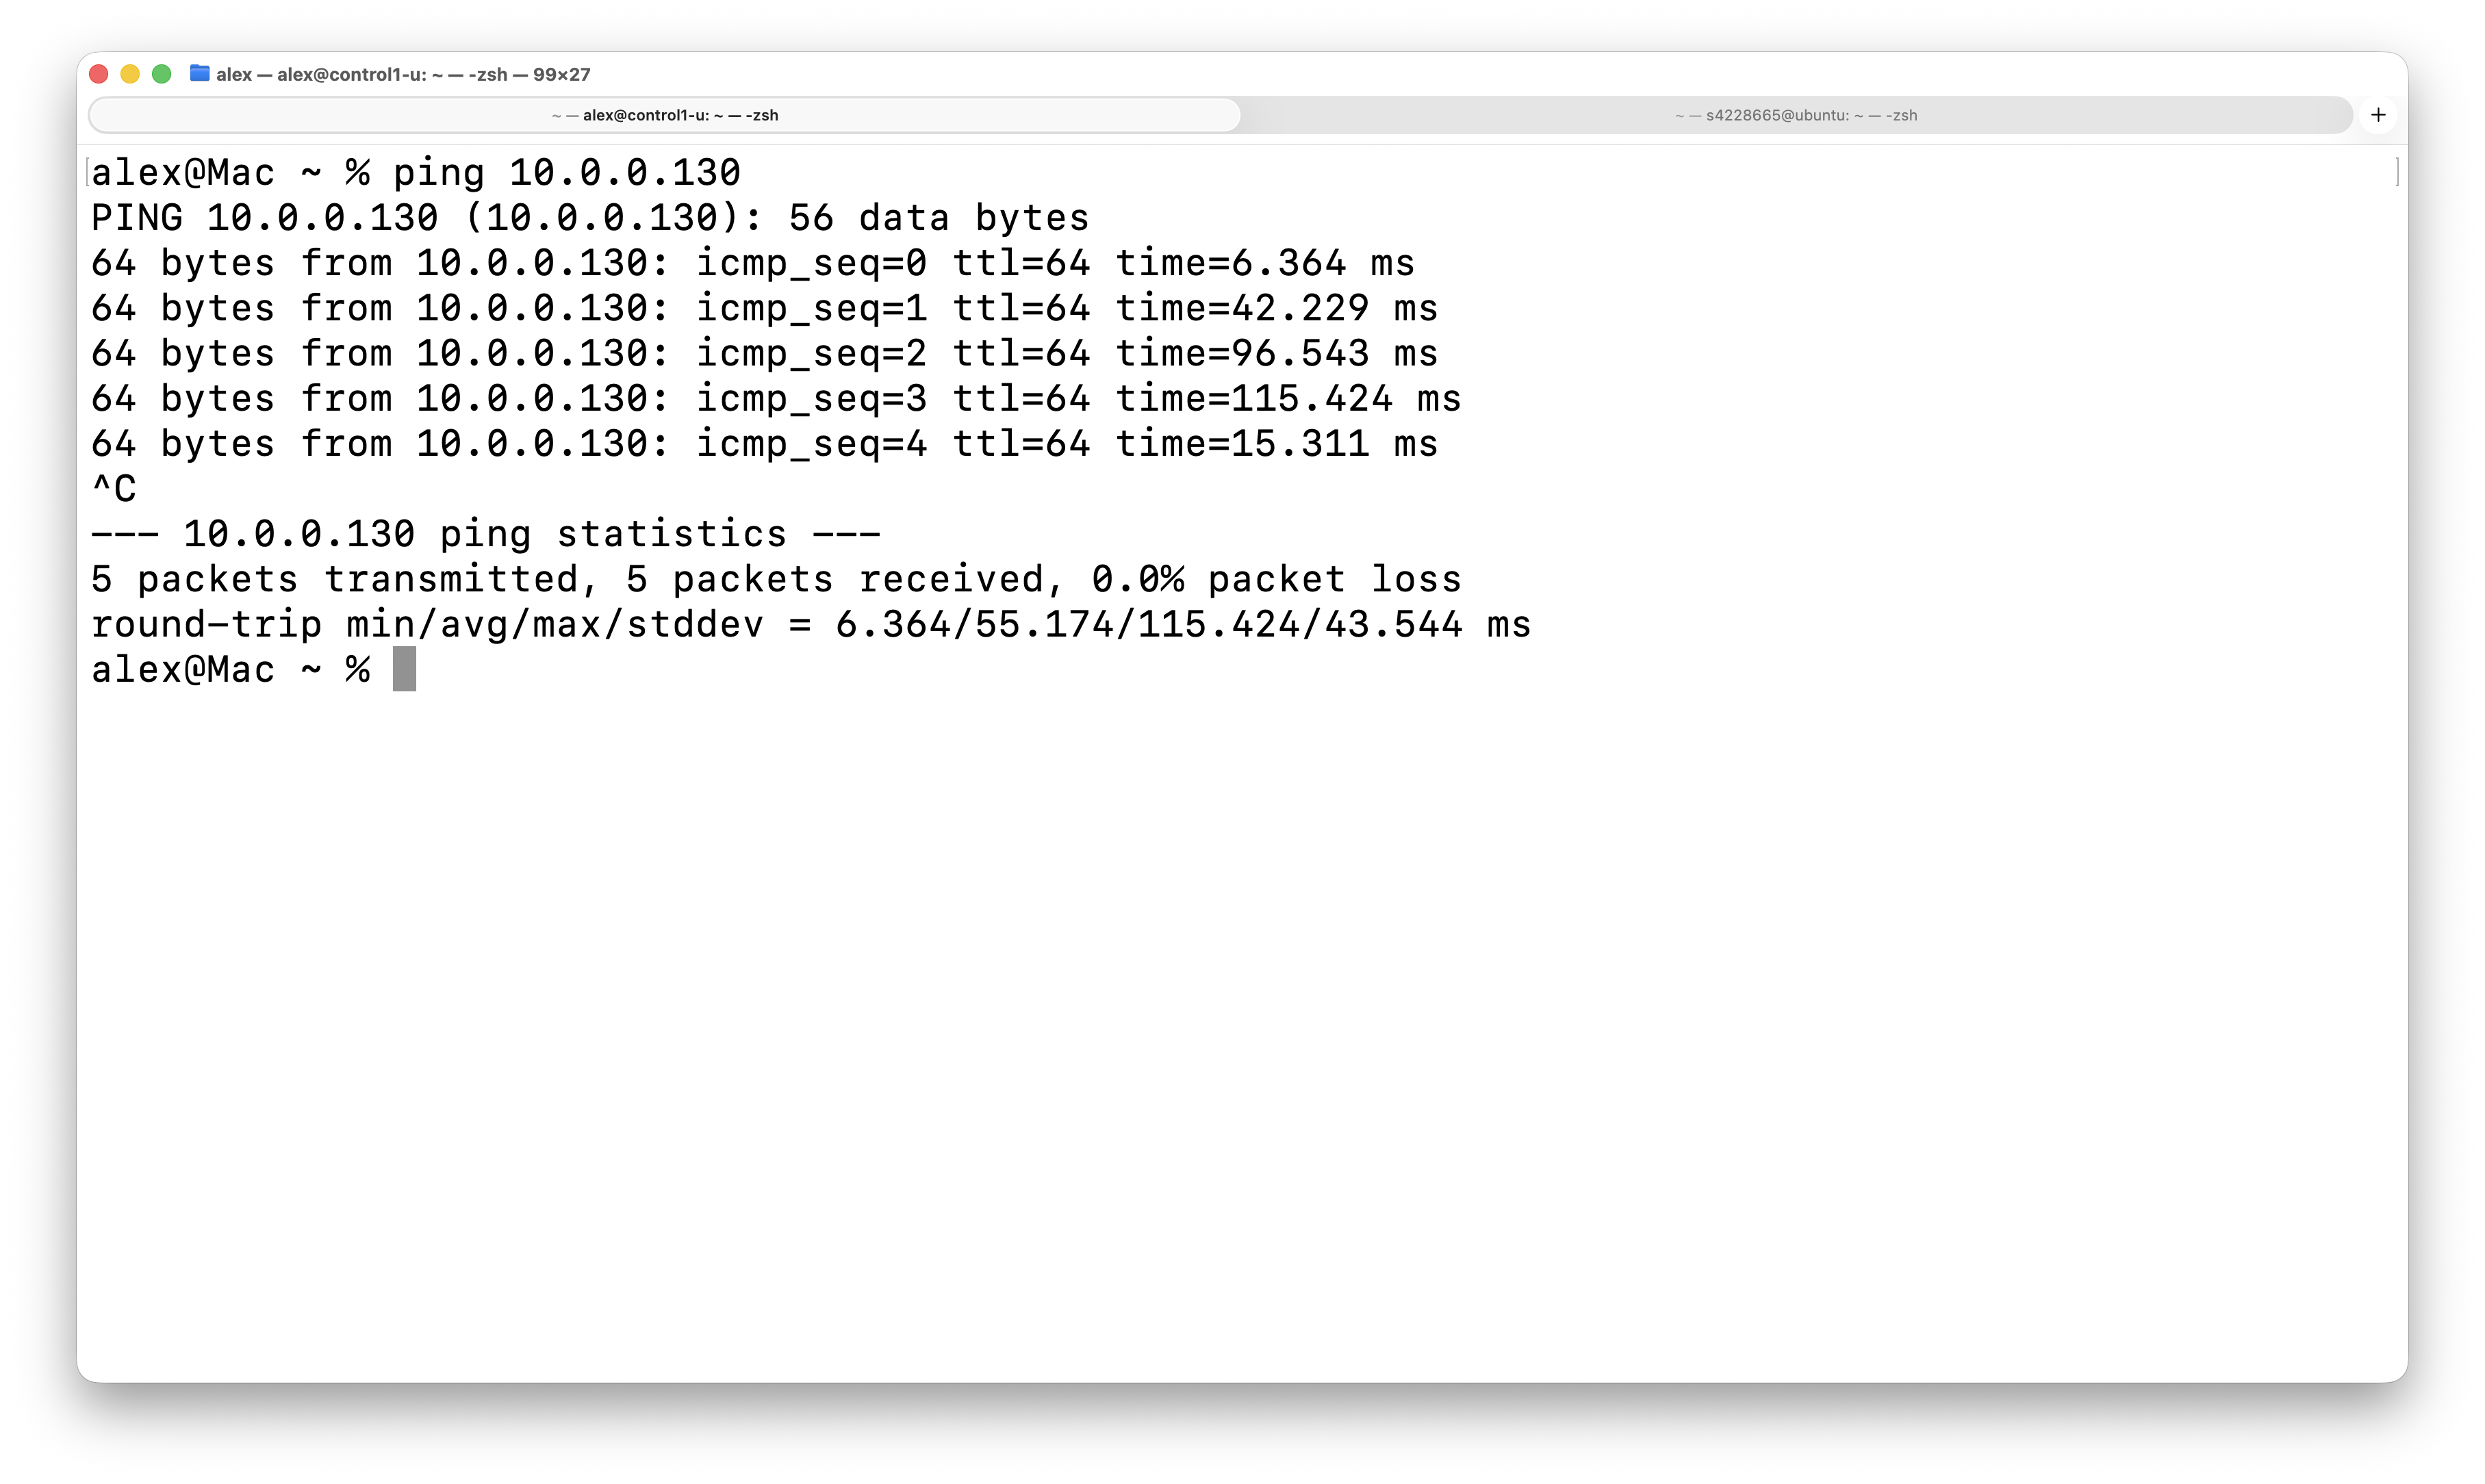
\includegraphics[width=0.8\linewidth]{Examples/iptables-ping-before.png}
  \captionof{figure}{A successful ping from my laptop to the Raspberry Pi}
  \label{example:iptables-ping-before}
\end{figure}

Since that has been validated, we can now put the rule in place to block the traffic, this is done using an iptables command but the coursework implementation will have this persisted using a file as seen later in section (TO DO REFERENCE DEPLOYMENT OF IPTABLES CONFIG FILE). The command for this is \verb|sudo iptables -A INPUT -p icmp -j DROP| which is to access the iptables cli, \verb|-A| to append to the \verb|INPUT| chain, \verb|-p| to specify we're dealing with \verb|icmp| traffic (protocol) and \verb|-j| to 'Jump' to a specified target, and we're going to \verb|DROP| it \parencite{Ubuntu2024IptablesHowTo}.

To validate the host is online and not just off (as ping tests are used to determine if a host is online) we can add a second rule to log the dropped packets, at base iptables does not log unless specified, so we can add a rule to log what happens to the incoming icmp traffic (CITATION). This command is \verb|sudo iptables -A INPUT -p icmp -j LOG --log-prefix "Blocked_icmp"|, the same levels of access as the previous rule to append to the \verb|input| chain but the \verb|-j| is jumping to the \verb|LOG| target where we can append the log using \verb|--log-prefix| with \verb|Blocked_icmp| to grep though system logs later.

\begin{figure}[H]
  \centering
  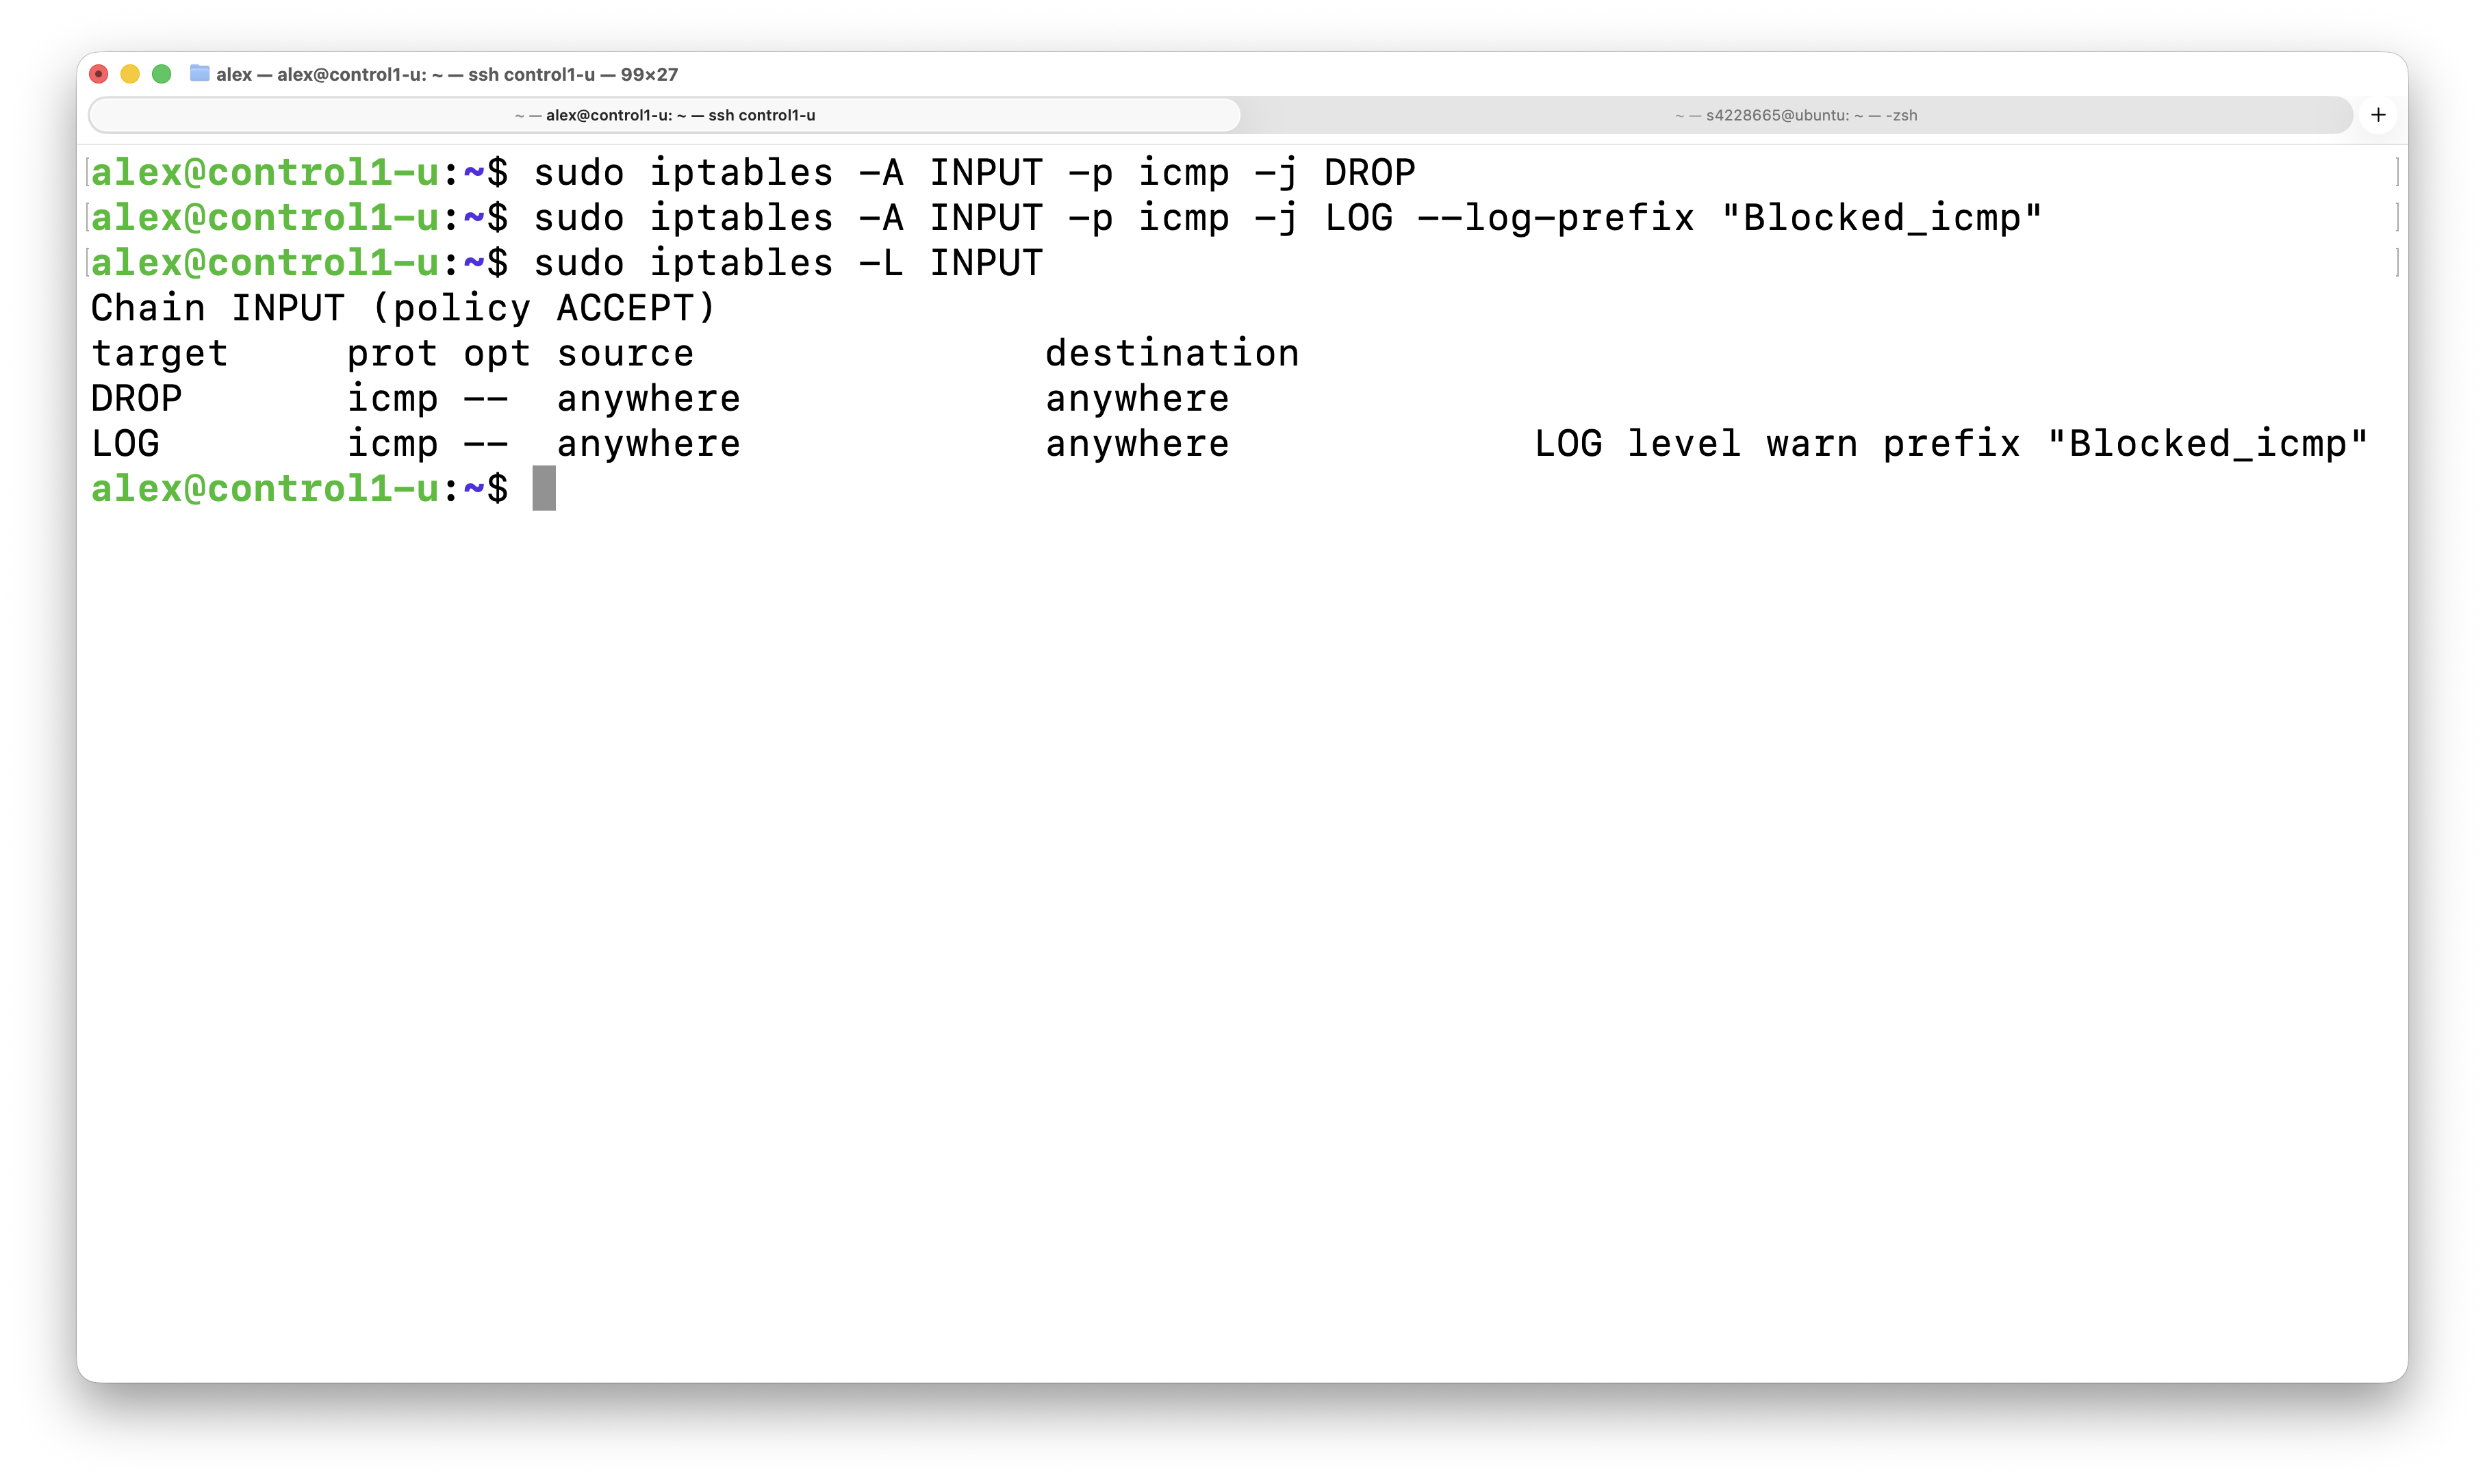
\includegraphics[width=0.8\linewidth]{Examples/iptables-ping-rules.png}
  \caption{Iptables rule in place to block all incoming icmp traffic  another to log the packets}
  \label{example:iptables-rules}
\end{figure}

We can now check this by sending icmp traffic to the now basic firewall and check the logs (stored in \verb|/var/log/syslog| by default) to see how the firewall dealt with the packets.

\begin{figure}[H]
    \centering
    \begin{subfigure}[b]{0.49\textwidth}
        \centering
        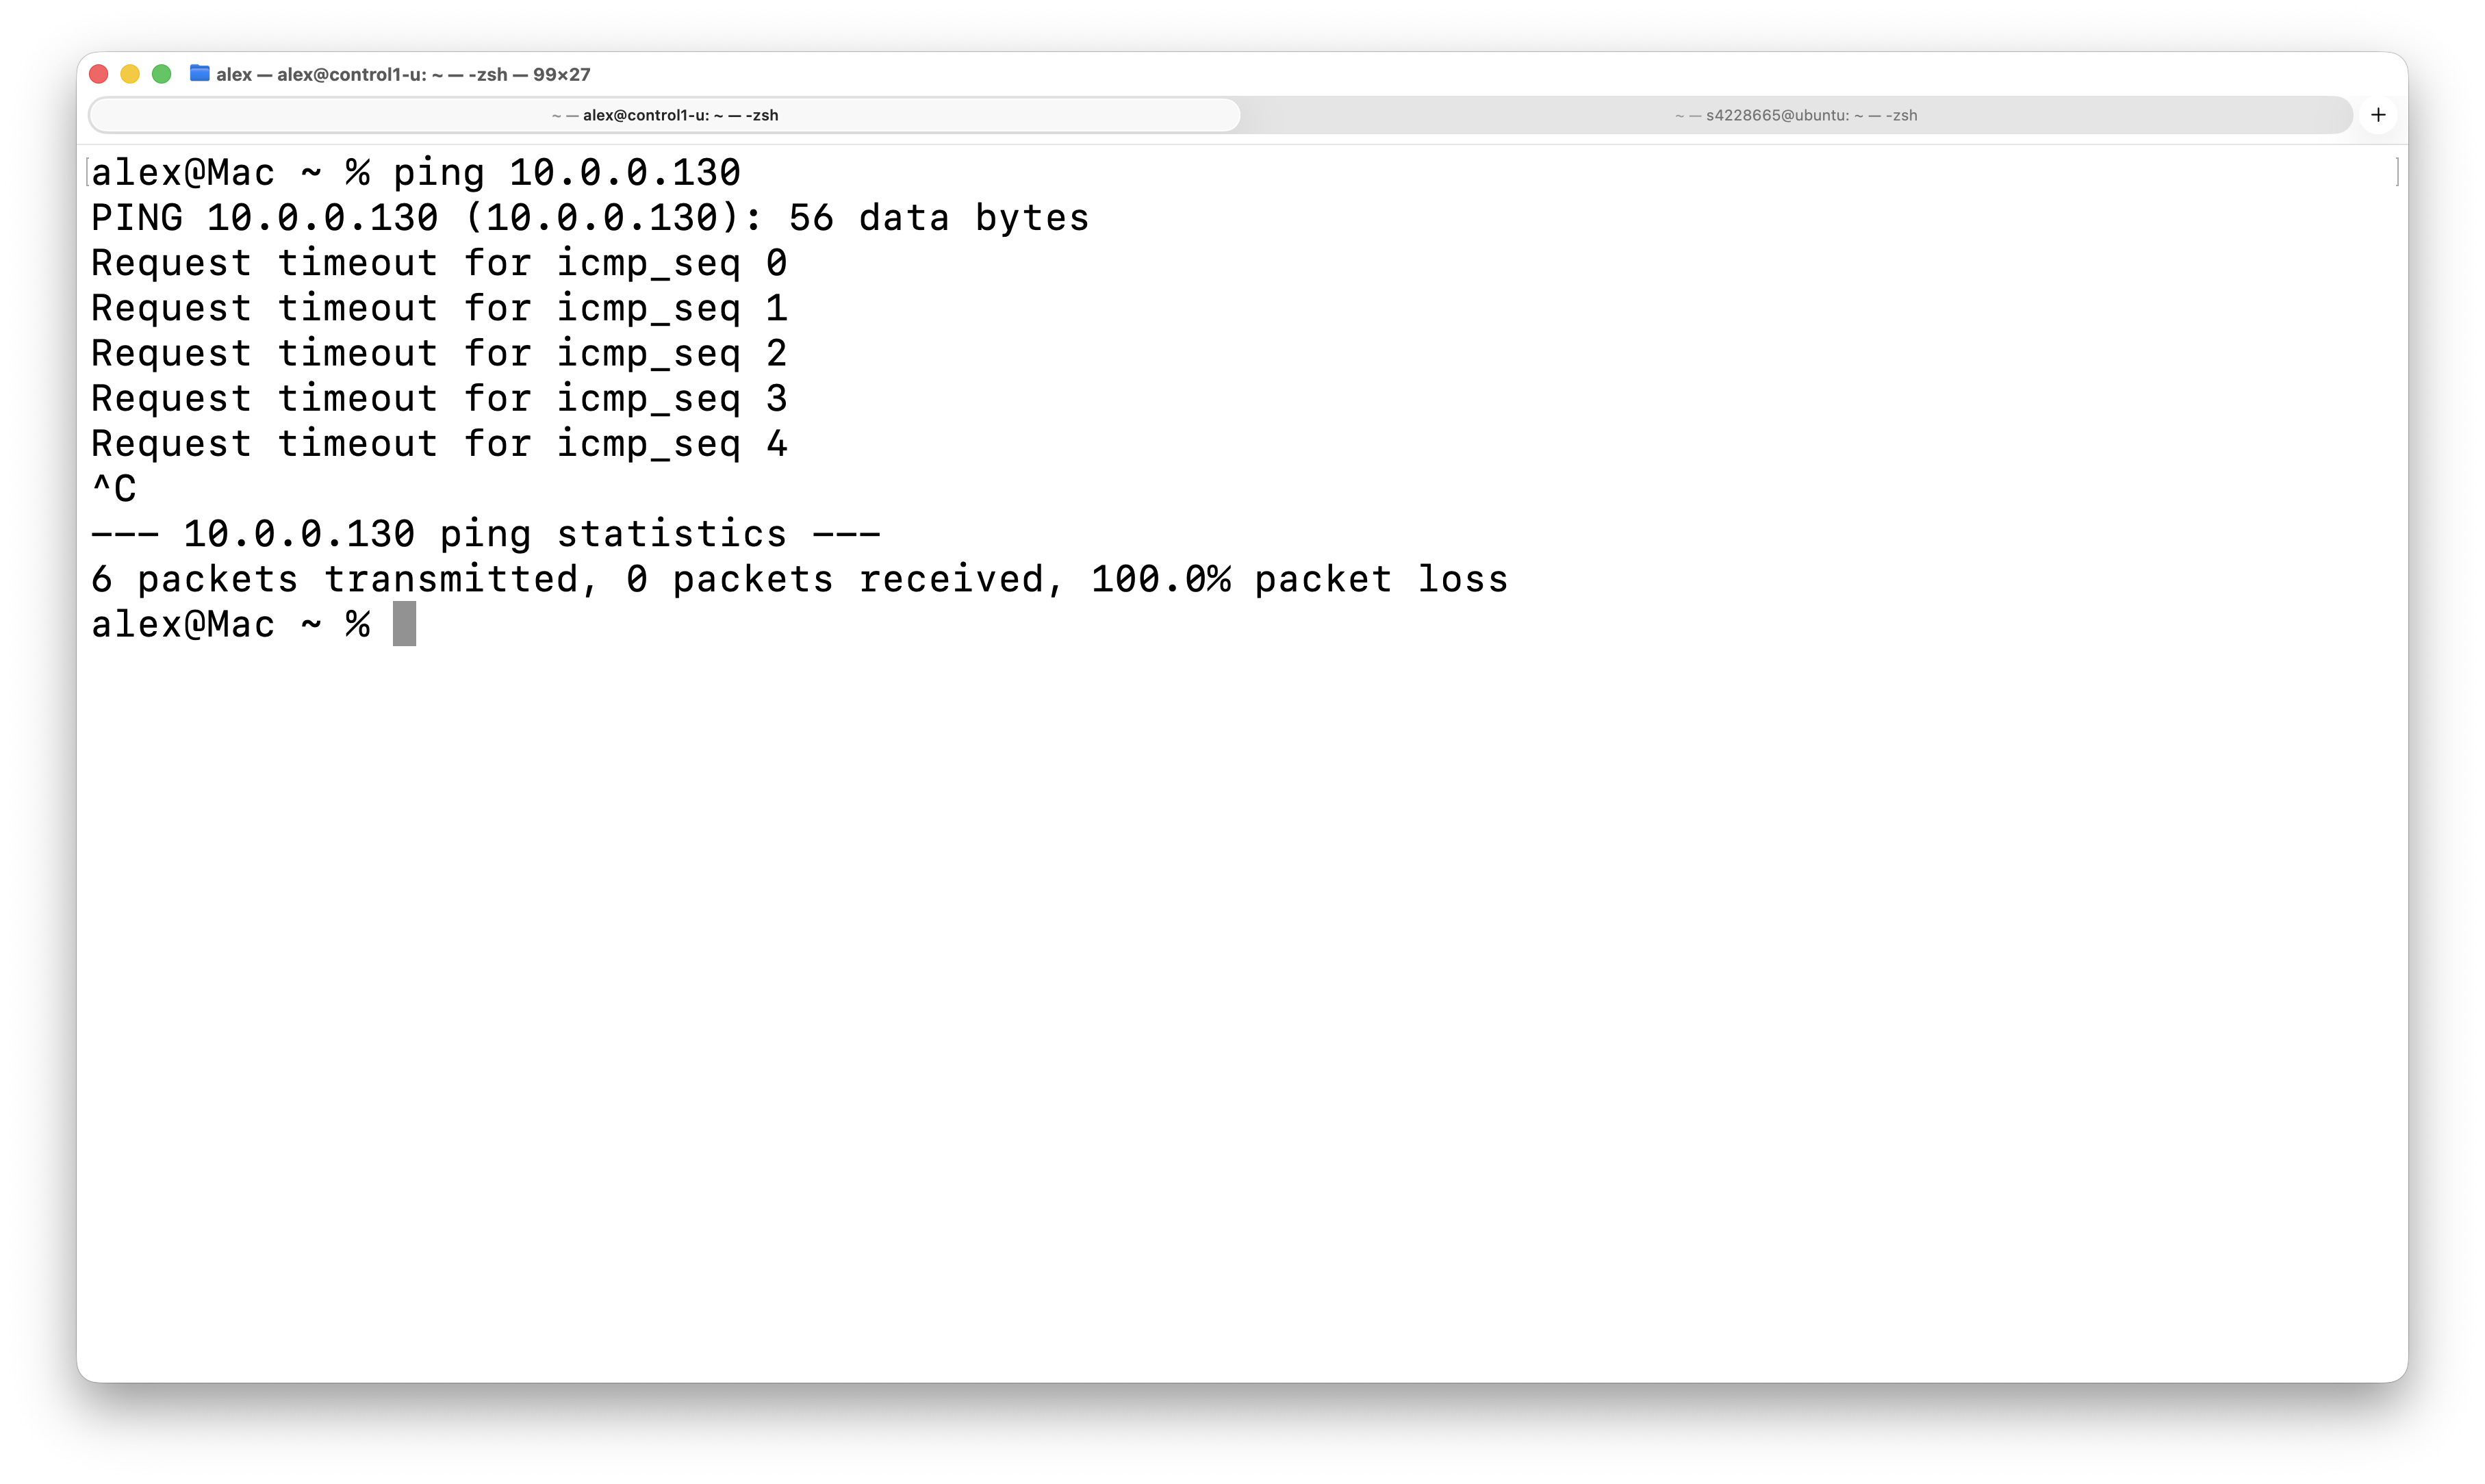
\includegraphics[width=\textwidth]{Examples/iptables-ping-blocked.png}
        \caption{A blocked successful ping from my laptop to the Raspberry Pi}
        \label{example:iptables-ping-blocked}
    \end{subfigure}
    \hfill
    \begin{subfigure}[b]{0.49\textwidth}
        \centering
        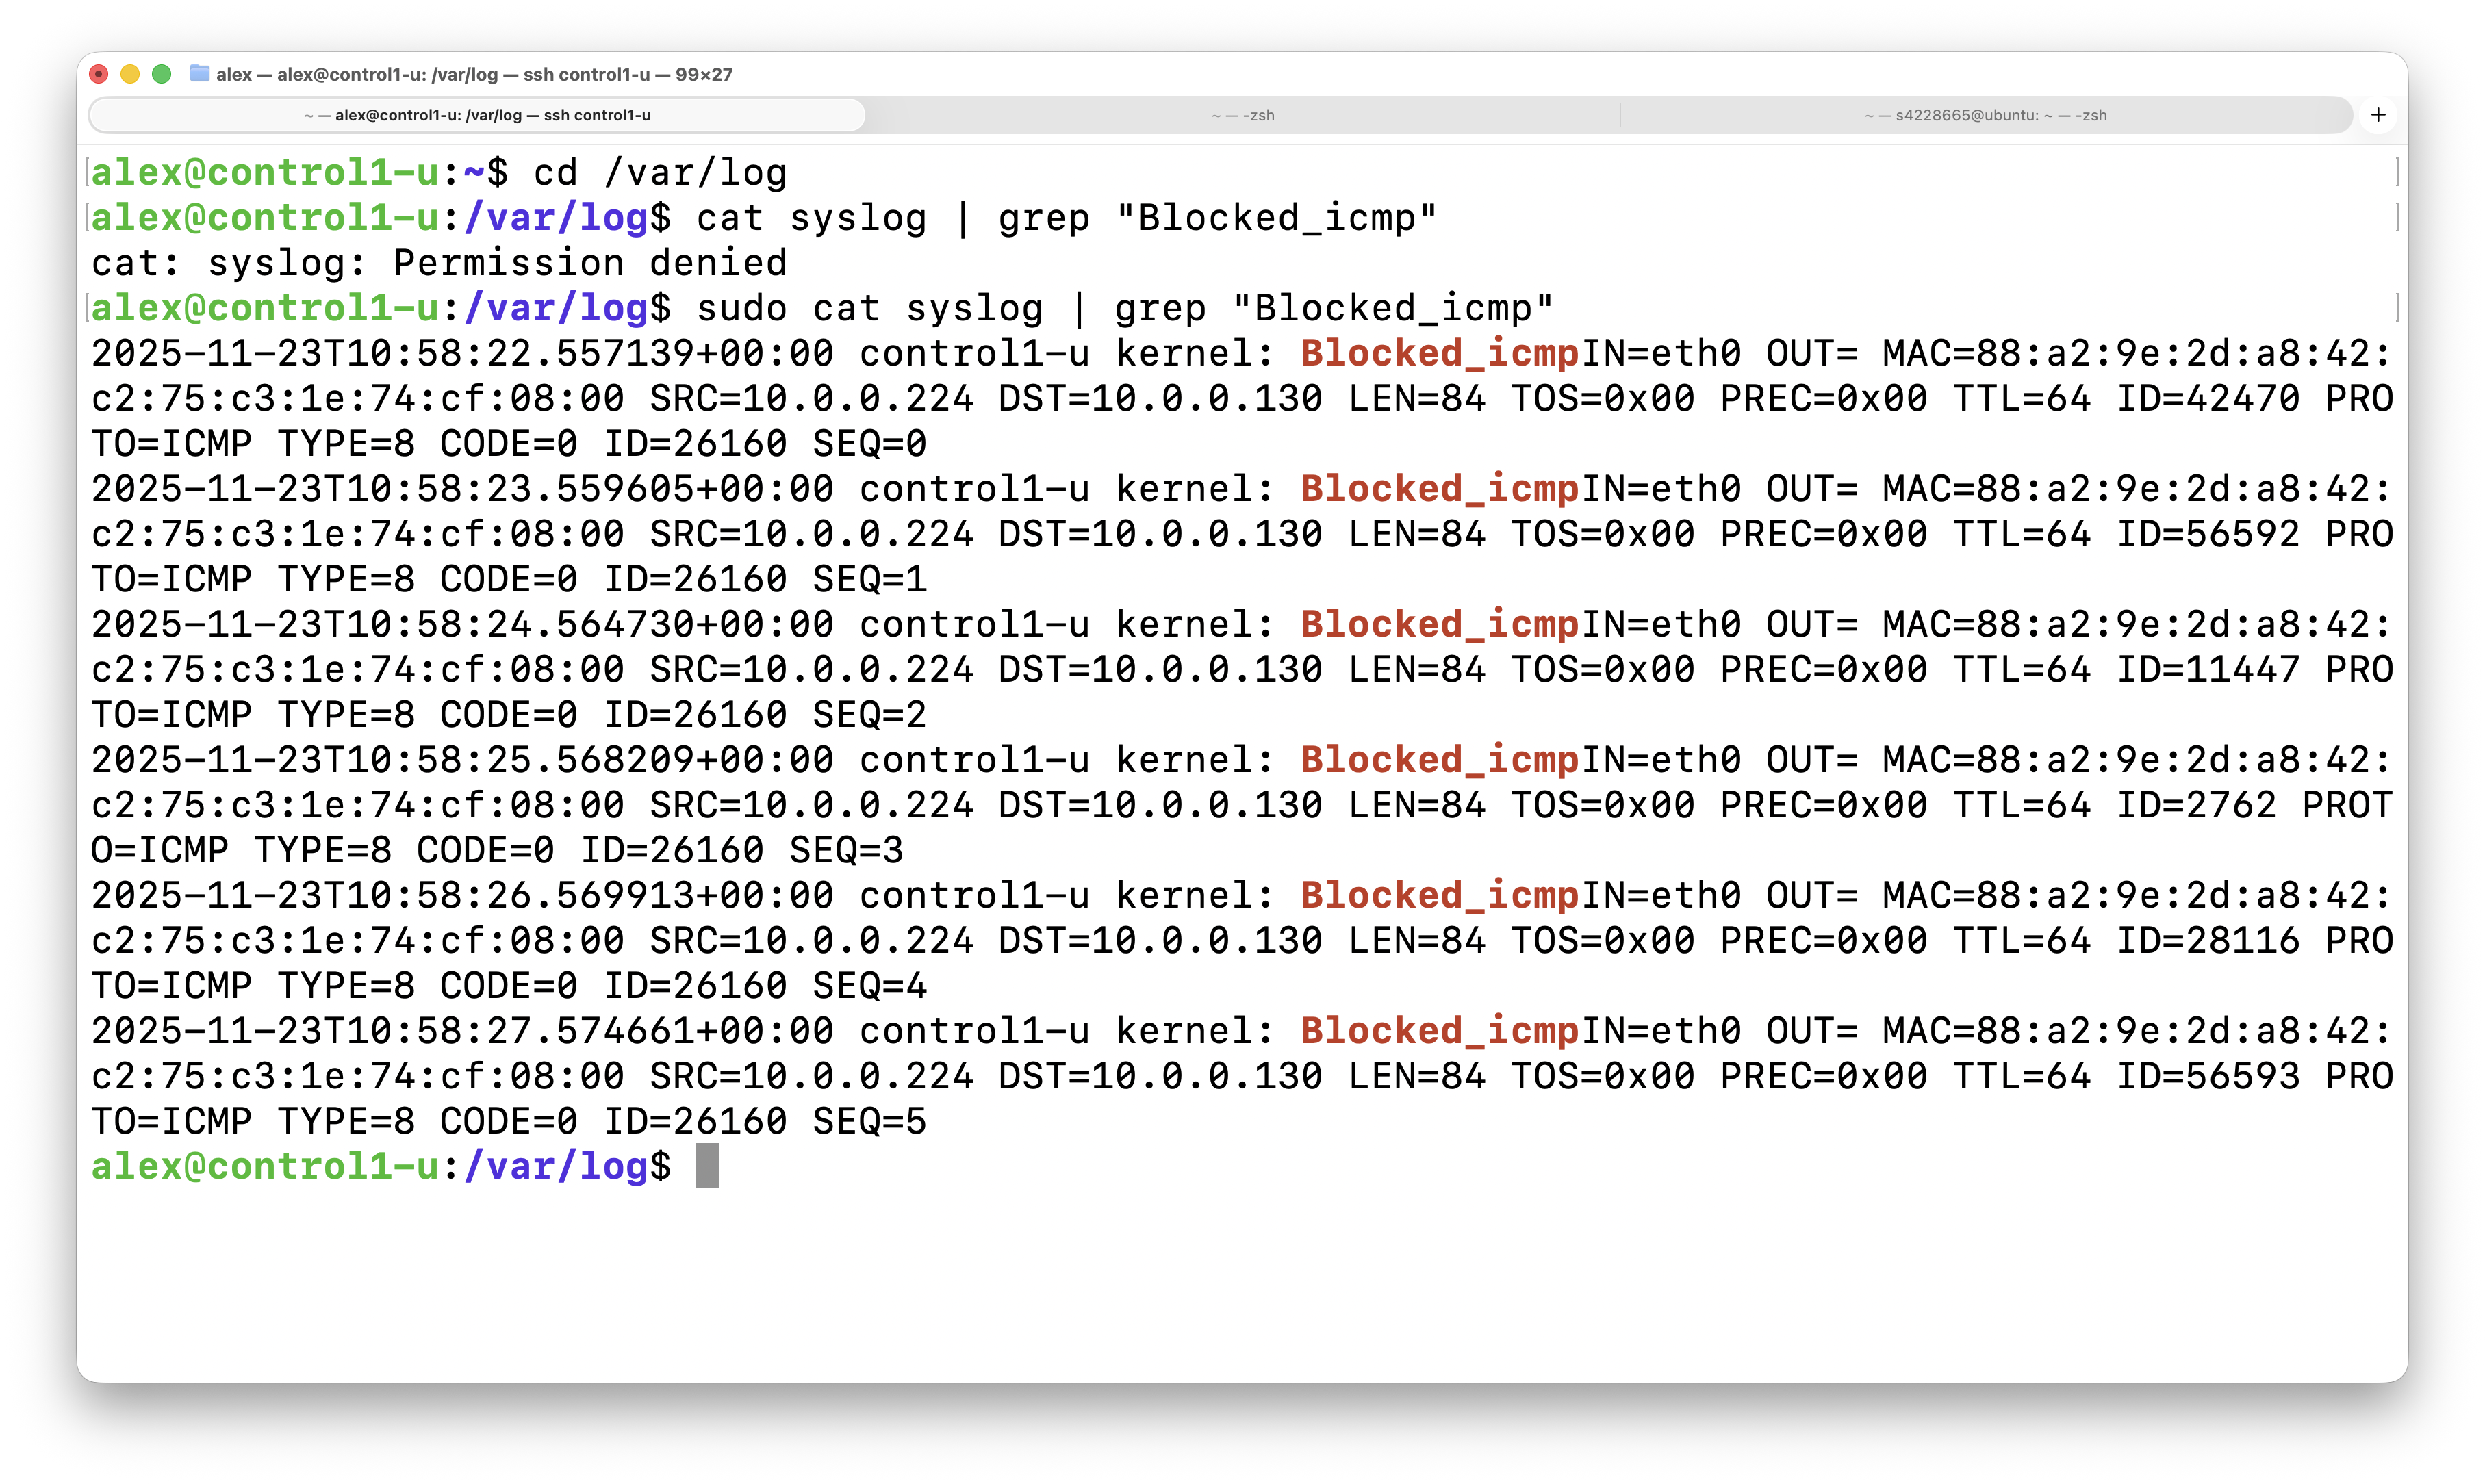
\includegraphics[width=\textwidth]{Examples/iptables-ping-logs.png}
        \caption{Logs from the iptables rule showing the dropped packets}
        \label{example:iptables-logs}
    \end{subfigure}
    \caption{Side-by-side view of the blocked ICMP traffic and the corresponding iptables logs}
    \label{fig:side-by-side-iptables-1}
\end{figure}

We can see the blocked pings in \ref{example:iptables-ping-blocked} and the corresponding logs in \ref{example:iptables-logs}. While iptables can't show the actions taken for each packet, the start of both rules (\verb|iptables -A INPUT -p icmp|) links them as they're both dealing with \verb|icmp| packets. From this we can also see the following about the packet:
\begin{itemize}
    \item The source's (My laptop) MAC address \verb|MAC=88:a2:9e:2d:a8:42:c2:75:c3:1e:74:cf:08:00|
    \item The source's IP address \verb|SRC=10.0.0.224|
    \item The destination's (My Pi) IP address \verb|DST=10.0.0.130|
    \item The protocol \verb|PROTO=ICMP|
\end{itemize}

As I use icmp packets to confirm if the Pi is online, I will remove the rules and validate packets are able to flow as intended in figures \ref{example:iptables-ping-after} and \ref{example:iptables-after}.

\begin{figure}[H]
    \centering
    \begin{subfigure}[b]{0.49\textwidth}
        \centering
        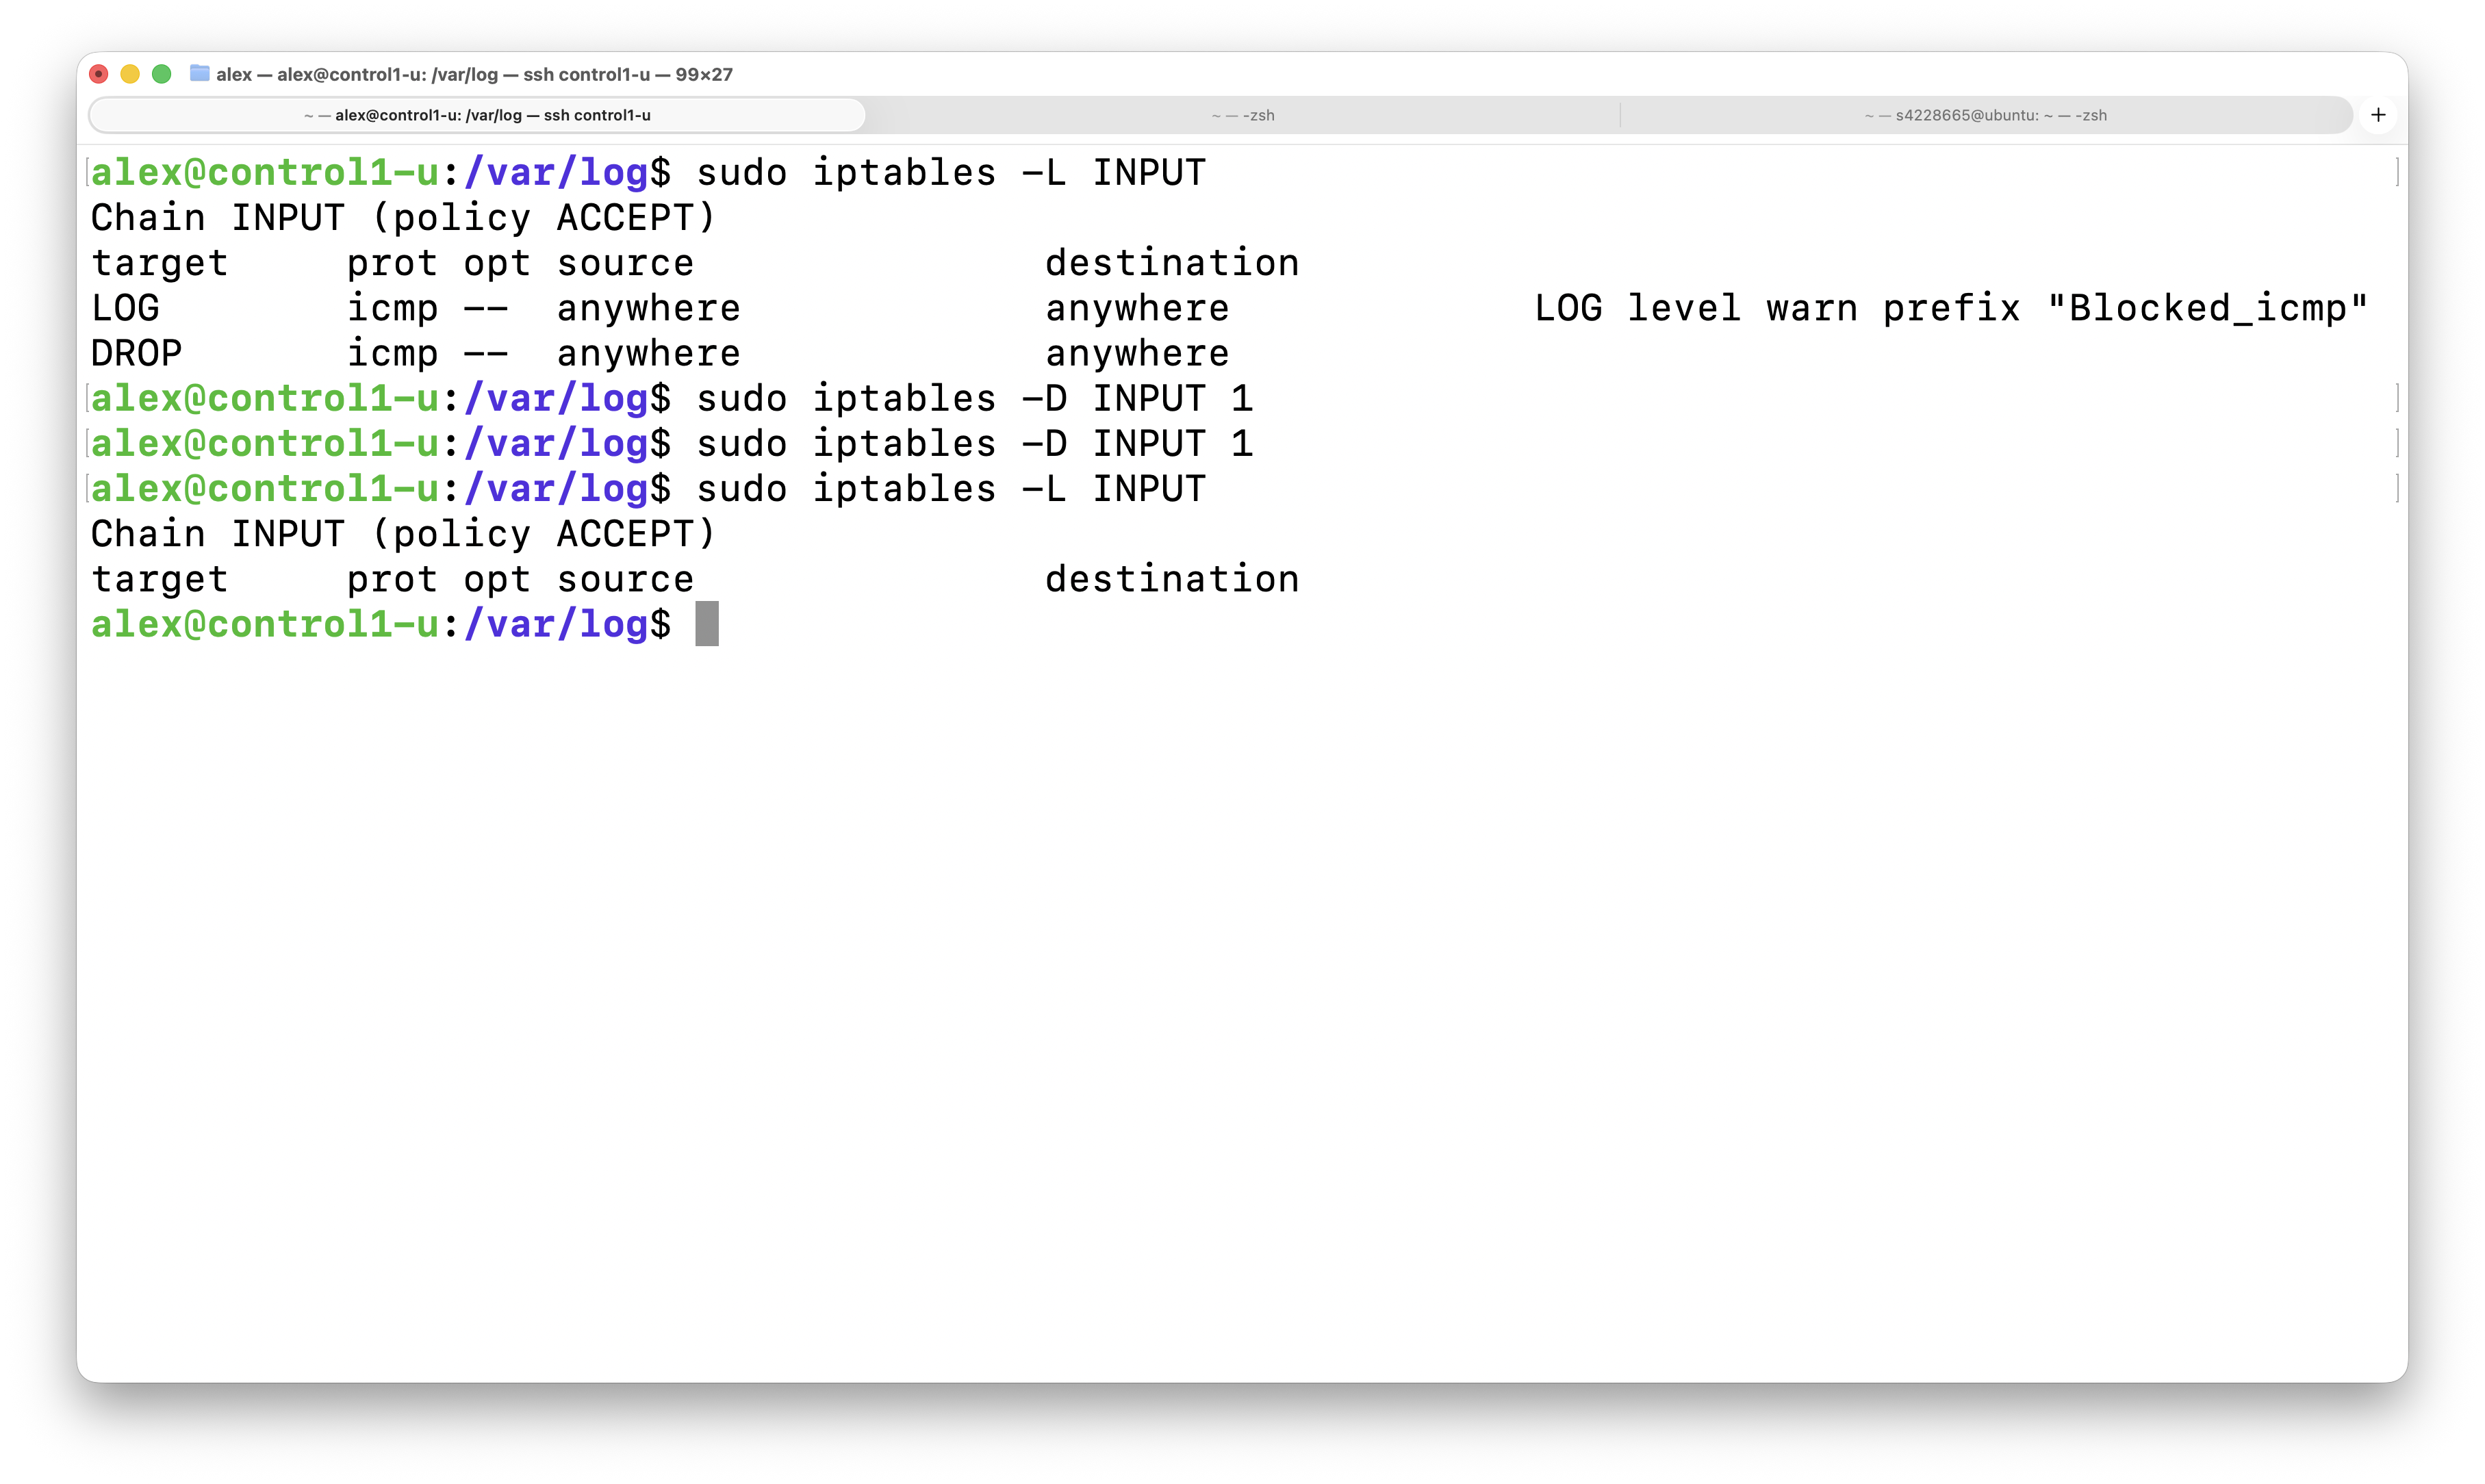
\includegraphics[width=\textwidth]{Examples/iptables-ping-cleanup.png}
        \caption{Both icmp iptables rules deleted showing zero 'input' rules}
        \label{example:iptables-ping-after}
    \end{subfigure}
    \hfill
    \begin{subfigure}[b]{0.49\textwidth}
        \centering
        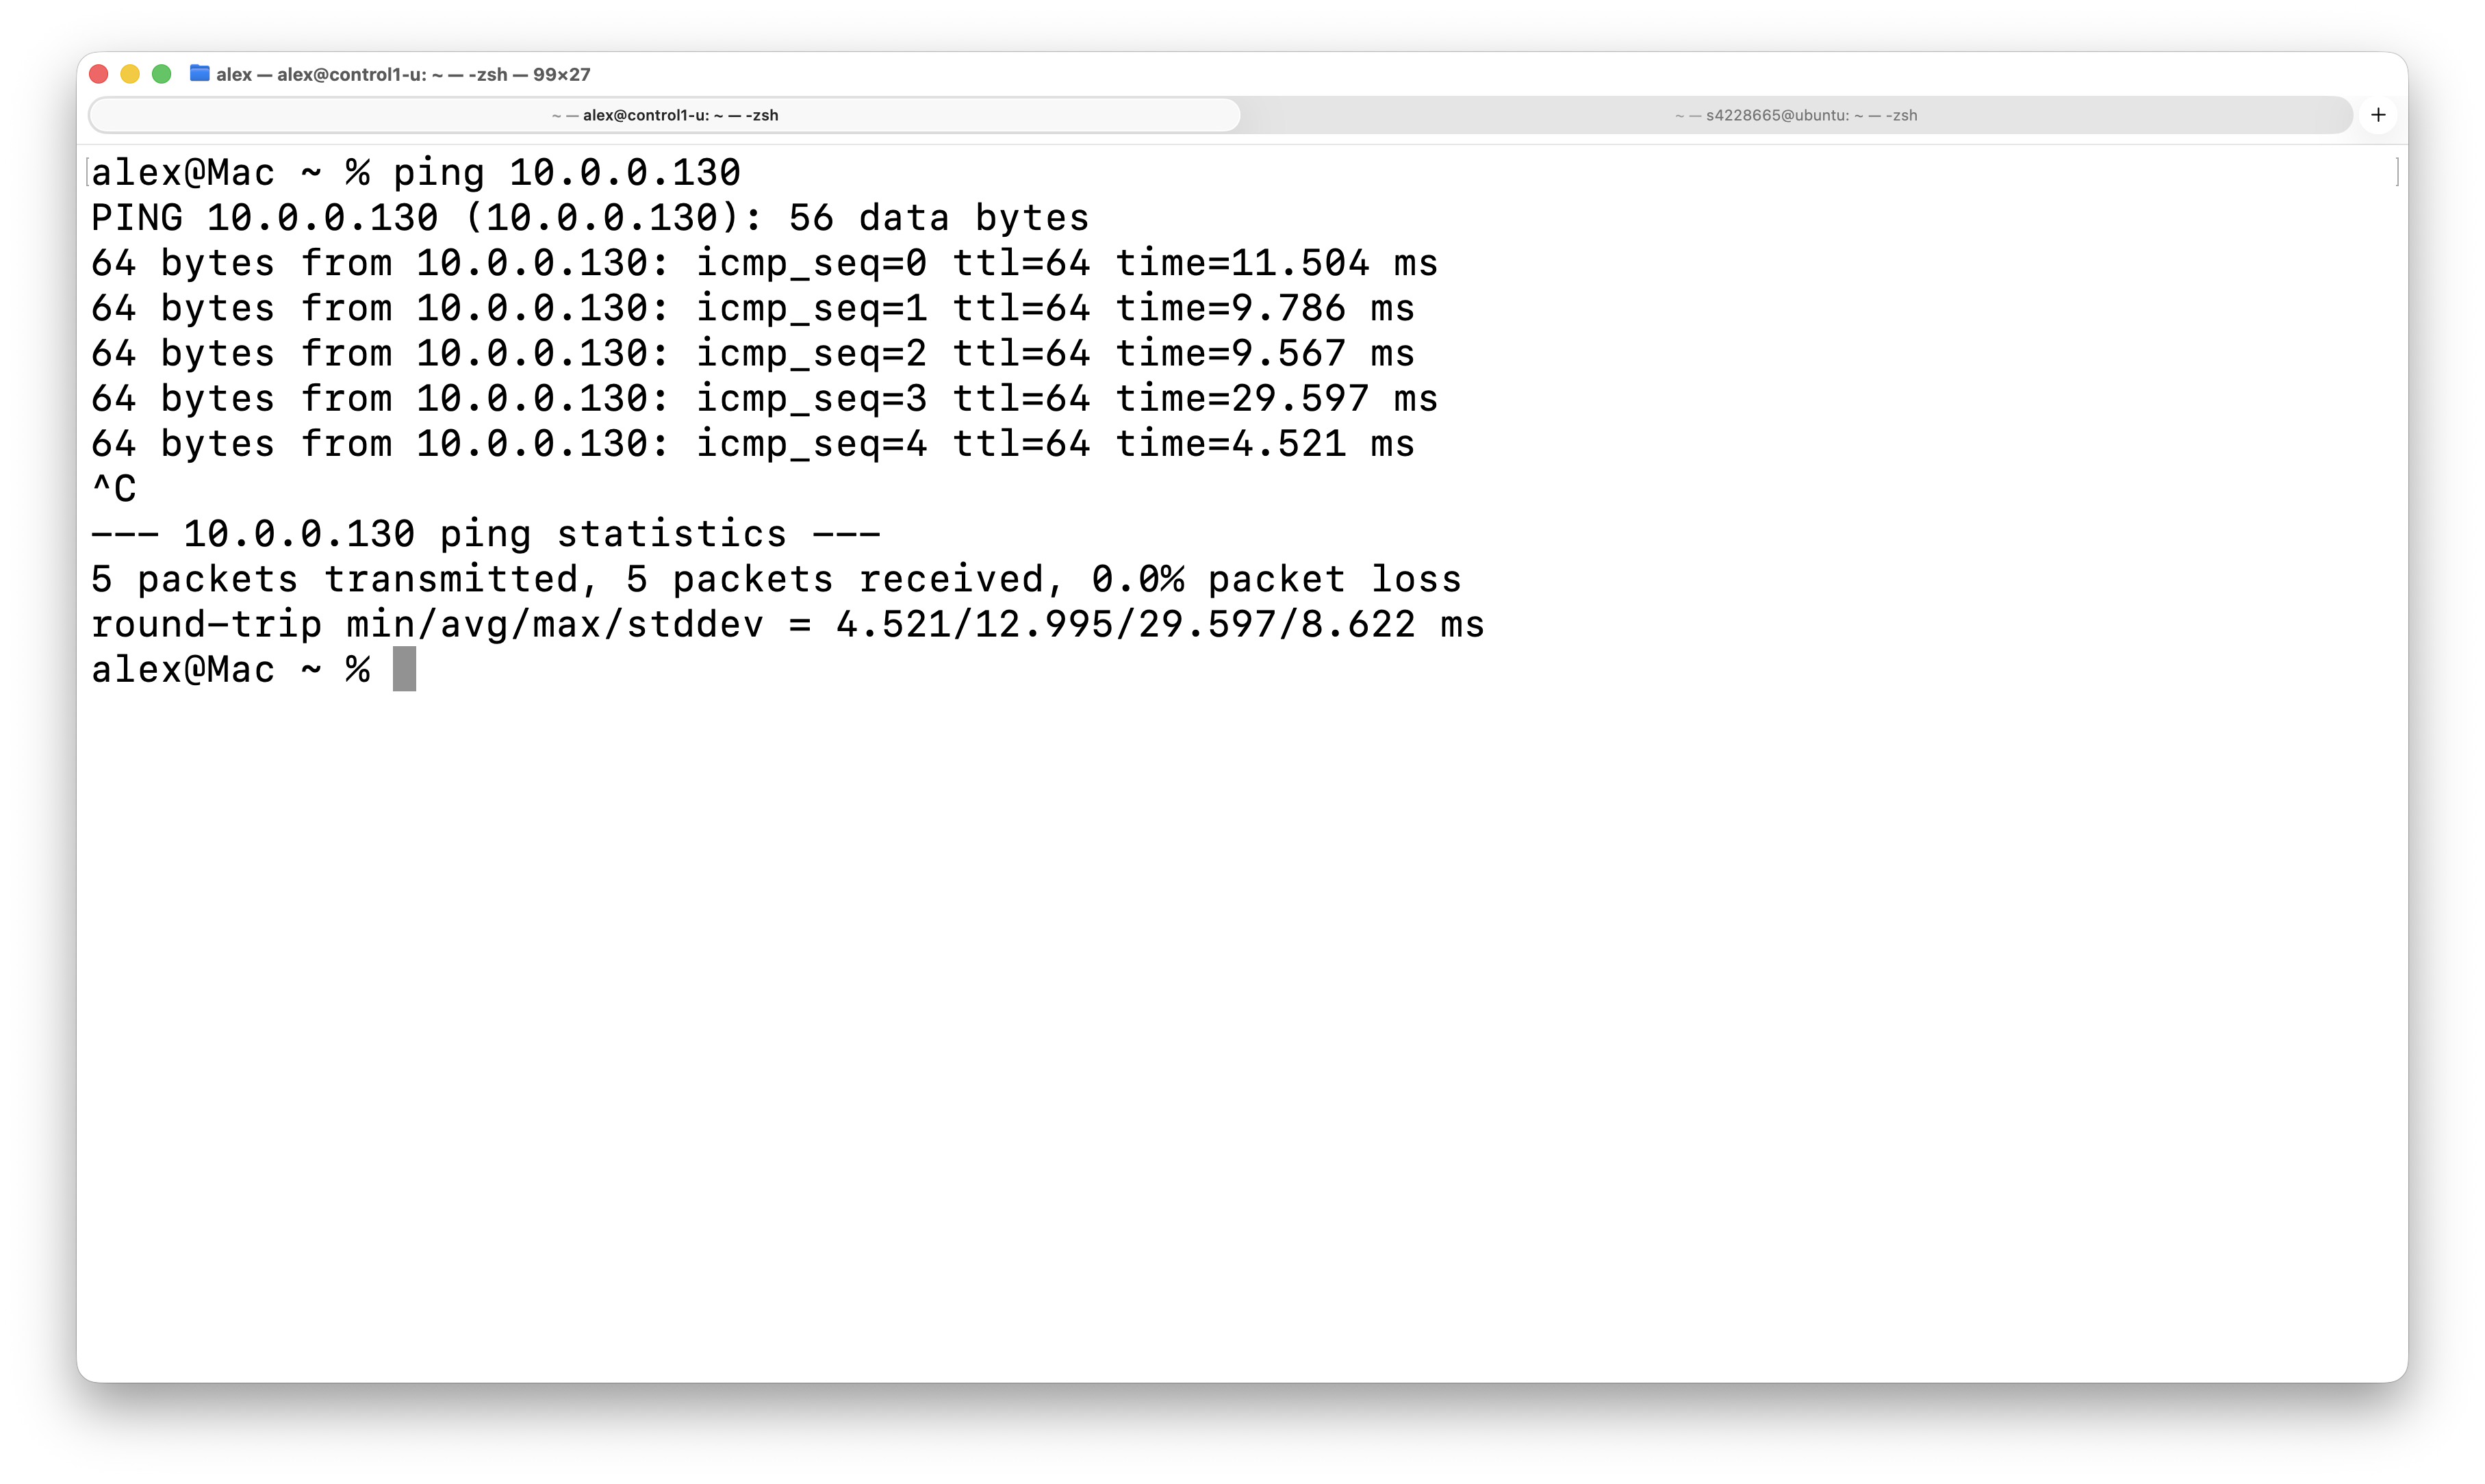
\includegraphics[width=\textwidth]{Examples/iptables-ping-after.png}
        \caption{Successful pings hitting the Pi after the icmp blocking rules were removed}
        \label{example:iptables-after}
    \end{subfigure}
    \caption{Side-by-side view of normal ICMP moving without the rules applied}
    \label{fig:side-by-side-iptables-finish}
\end{figure}

\subsection{What is Netplan?}
Netplan is Ubuntu's network configuration abstraction renderer \parencite{Netplan2024Official}. It allows the abstracted definition of network interfaces on a Ubuntu system by allowing administrators to define the following on a network interface using YAML, it lets you define the:
\begin{itemize}
    \item TCP/IP information address of the host
    \begin{itemize}
        \item IPv4/v6 Address and subnet masks
        \item DNS server(s)  
    \end{itemize}
    \item Default gateway (via default route)
    \item Static routes
    \item Search Domains
\end{itemize}

As a method of abstraction, netplan interfaces with lower-level daemons (NetworkManager and Systemd-networkd) to handle the real networking and interface directly with the Linux kernel as per figure \ref{fig:netplan_design}. TODO EXPAND AND RESEARCH THIS

\begin{figure}[H]
    \centering
    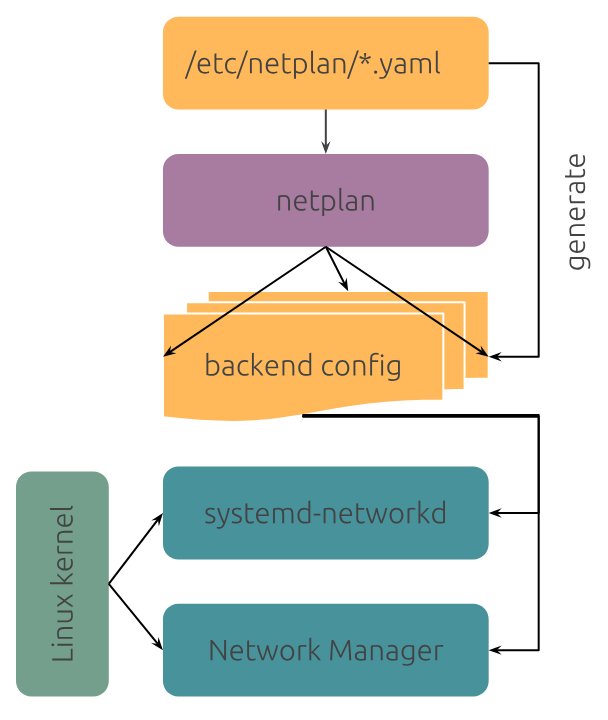
\includegraphics[width=0.4\linewidth]{Diagrams/os-netplans-hld.png}
    \caption{Netplan Design Overview}
    \parencite{Ubuntu2024NetplanDesign}
    \label{fig:netplan_design}
\end{figure}

\begin{figure}[H]
    \centering
    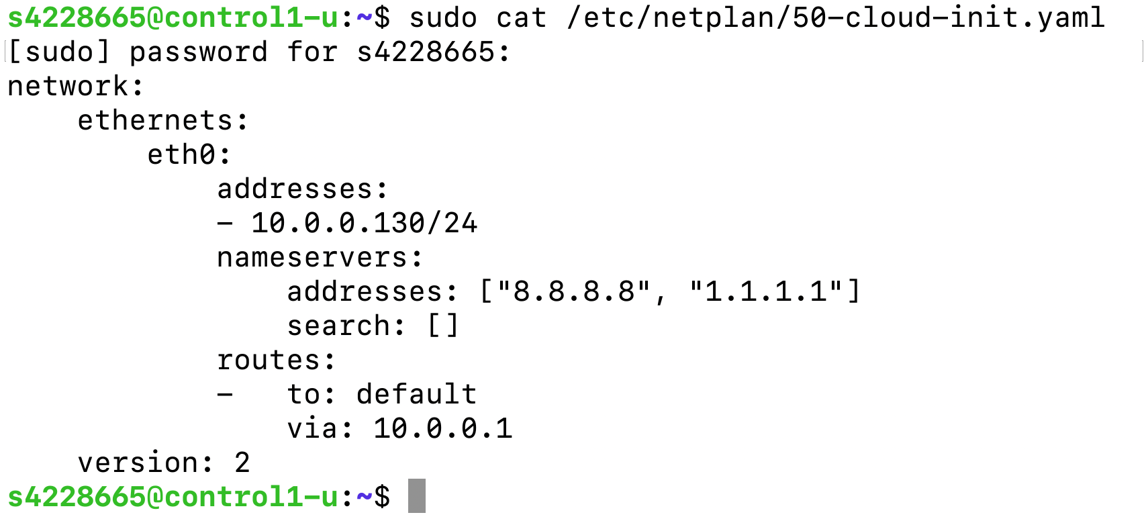
\includegraphics[width=0.75\linewidth]{Report_Images/os-netplan-screenshot.png}
    \caption{A netplan file}
    \label{fig:netplan-example}
\end{figure}

A rendered netplan file (figure \ref{fig:netplan_design}) showing a Pi's network config from the \verb|eth0| interface connected to network \verb|10.0.0.0/24| with IPv4 address \verb|10.0.0.130| using DNS servers \verb|8.8.8.8| and \verb|1.1.1.1| (owned and maintained by Google and Cloudfare), no search domain configured and default gateway (default route) at \verb|10.0.0.1|. This example was taken from the same Raspberry Pi (not the coursework-provided one) as shown in figure \ref{fig:UFW-example}.

\subsection{System Requirements and Design}
\label{subsec:system-requirements}

\subsubsection{Hardware Requirements}
As the firewall device is implemented using Ubuntu Server, base hardware requirements are incredibly low, sitting at:
\begin{itemize}
    \item 1.5 GB of RAM
    \item 5 GB of storage
\end{itemize}
While these are minimum specs, it would be better to have more resources than these; the Ubuntu docs mention having 3 GB (or more) of RAM and 25 GB (or more) for storage as recommended \parencite{Ubuntu2024SystemRequirements}. As for CPU specs, the official website does not even specify a CPU constraint/requirement. It instead shows supported 64-bit and 32-bit architectures which are:
\begin{itemize}
    \item amd64 (64-bit Intel/AMD)
    \item amd64 (64-bit Arm) - This is the type of CPU Raspberry Pi has
    \item armhf (32-bit Arm)
    \item ppc64el (64-bit Power)
    \item riscv64 (64-bit RISC-V)
    \item s390x (64-bit Mainframe)
\end{itemize}

\subsubsection{Hardware Overview}
The Raspberry Pi provided for this coursework is a Model 4B (with 4GB of RAM). This model has the following hardware specs:
\\Processing and Memory:
\begin{itemize}
    \item SoC: Broadcom BCM2711, Quad-core ARM Cortex-A72 (ARMv8) 64-bit @ 1.8 GHz
    \item RAM: 4 GB LPDDR4-3200 SDRAM
    \item GPU: VideoCore VI (not used)
\end{itemize}
\\Network Interfaces:
    \begin{itemize}
    \item Onboard Gigabit Ethernet
    \item WiFi: Dual-band 802.11ac WiFi (2.4 GHz and 5.0 GHz)
    \item Bluetooth: Bluetooth 5.0, BLE (not used)
\end{itemize}
\\Expansion and Connectivity:
\begin{itemize}
    \item USB Ports: 2× USB 3.0 ports, 2× USB 2.0 ports (The USB 3 ports are used for the additional NIC)
    \item GPIO: 40-pin header (not used)
    \item Display: 2× micro-HDMI ports (not used past OS install)
    \item Storage: microSD card slot
\end{itemize}

\subsubsection{Network Interface Card Overview}
As shown in figure \ref{basic-fw-breakdown} and the coursework brief, there should be 3 network interface cards (NICs), each configured to have a different class network represented. The Raspberry Pi firewall is able to accommodate this with the two onboard NICs and an additional WiFi NIC provided with the Pi.
\paragraph{Interface 1 - WAN/Class A Network}
\begin{itemize}
    \item Hardware: Onboard Gigabit Ethernet port
    \item Linux Device/Name: \verb|eth0|
    \item Connection: Physically cabled up with an RJ45 cat6e cable
    \item Summary: 
\end{itemize}

\paragraph{Interface 2 - LAN2/Class B Network}
\begin{itemize}
    \item Hardware: Additional WiFi Dongle NIC
    \item Linux Device/Name: ???
    \item Connection:
    \item Summary: 
\end{itemize}

\paragraph{Interface 3 - LAN2/Class C Network}
\begin{itemize}
    \item Hardware:
    \item Linux Device/Name: \verb|wlan0|
    \item Connection:
    \item Summary: 
\end{itemize}










\subsubsection{Iptables and Netfilter Requirements}
Iptables is a userspace utility that accesses the Netfilter module in the kernel, so it does not have its own system overhead. It is a command-line interface to configure the Linux kernel's Netfilter module/framework directly. The netfilter project is a community-driven, collaborative, free and open-source software (FOSS) project that provides packet filtering, NAT, packet logging, and other packet management for the Linux 2.4.X and later Kernels \parencite{Netfilter2024Official}.

Netfilter itself operates as a kernel module (not the userspace), which means packet filtering happens in the kernel space, so 'standard' use of the Pi would be unaffected by the packet inspection, similar to how an enterprise router would work with a control plane (userspace) and a forwarding plane (kernel space) \parencite{Cloudflare2024ControlPlane}. As such, the only requirement is the Ubuntu 24.04 (the latest long-term support (LTS)) operating system has Linux kernel 2.4 or later built in - this has been supported for years, and the Linux kernel in Ubuntu 24.04 is 6.8 \parencite{Ubuntu2024KernelLifecycle}.

\section{Planning and Implementation}
\label{sec:implementation}

\subsection{Initial Setup and OS install}
\label{subsec:initial-install}
\subsubsection{Install - balenaEtcher}
\label{subsubsec:balena-install}
To start the install I used balenaEtcher \parencite{Balena2024Etcher} with a downloaded .iso disk image of Ubuntu server (24.04 LTS), figures \ref{fig:balena1}, \ref{fig:balena2} and \ref{fig:balena3} show the install process though balenaEtcher's ui to configure the OS, select the medium (again the coursework provided SD card) and begin the installation. However, figure \ref{fig:balena4} shows the bootloader after installing the OS and installing the SD card into the Pi, suggesting the install didn't go well.

\begin{figure}[H]
\centering
\begin{minipage}{.48\textwidth}
  \centering
  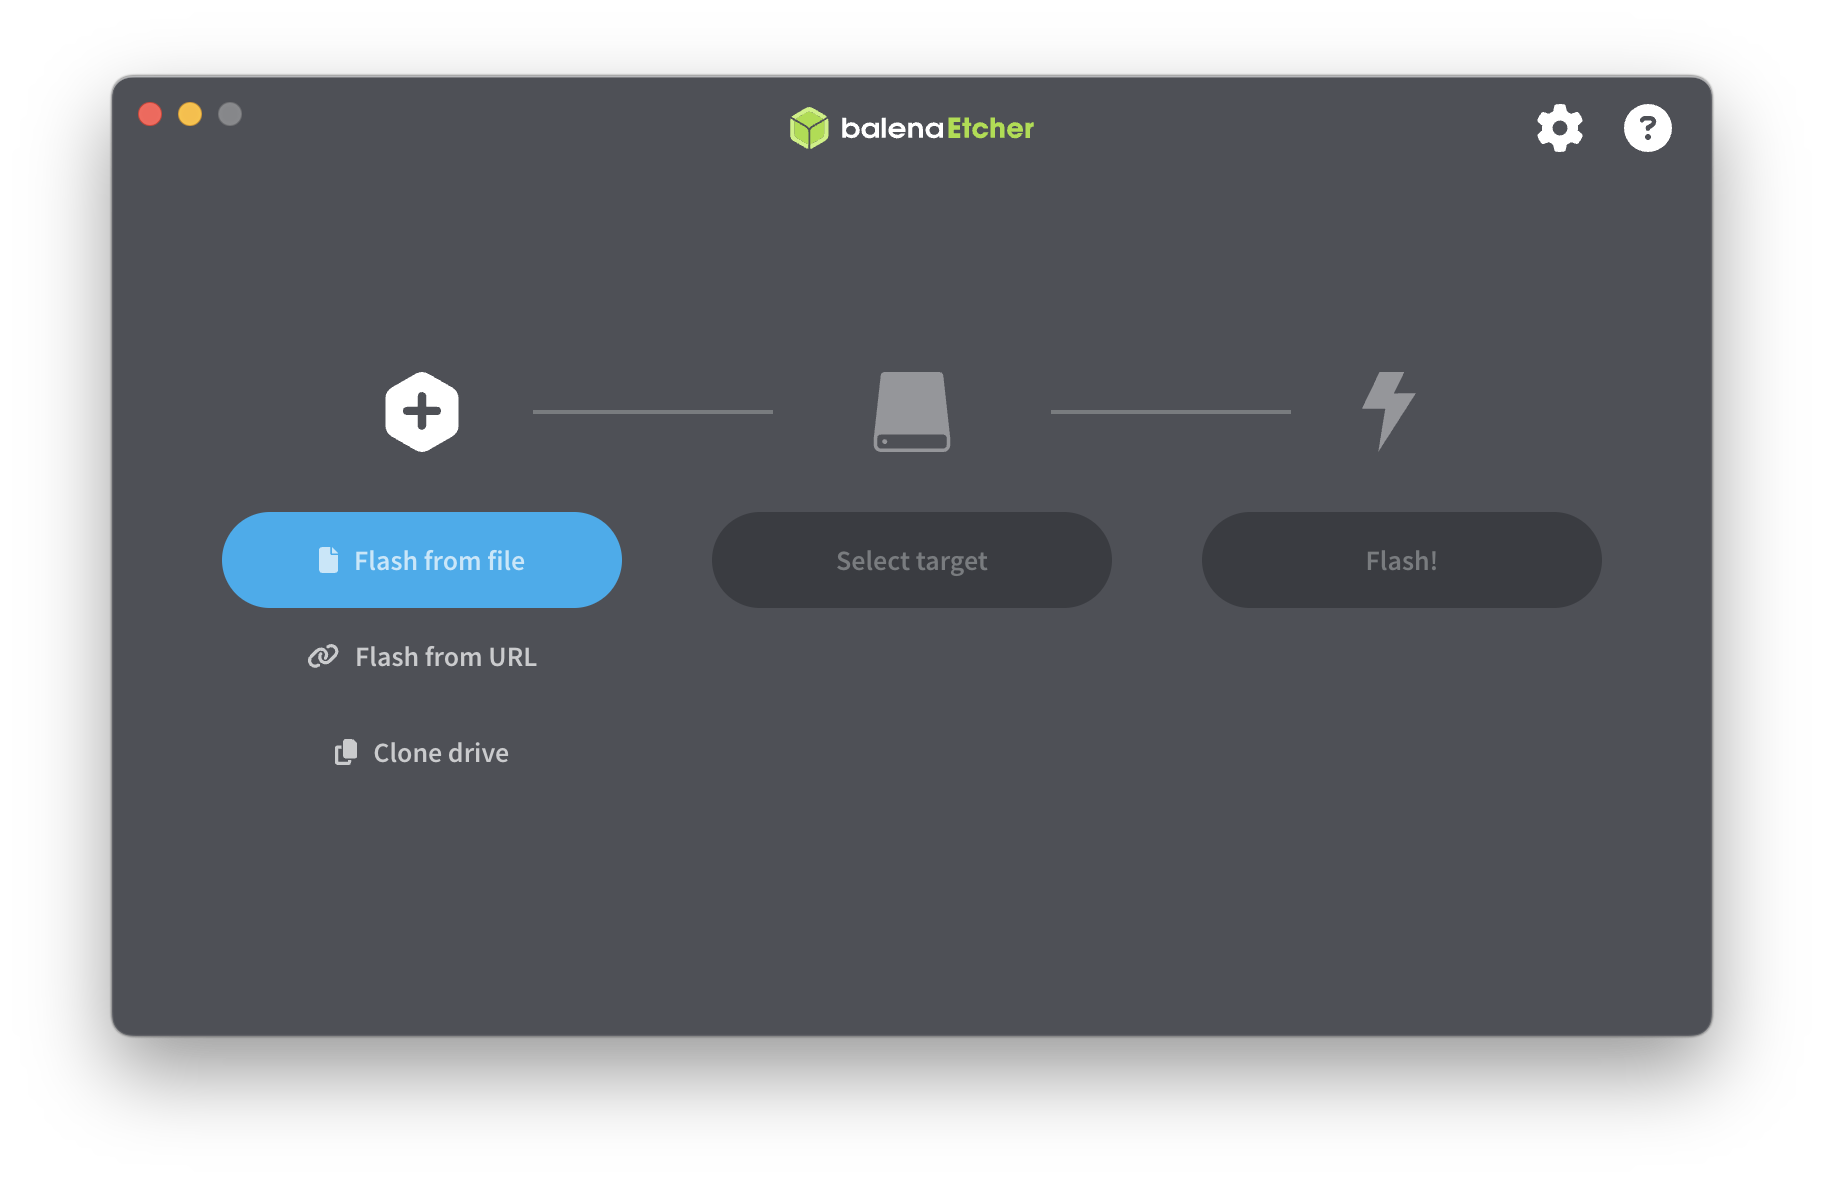
\includegraphics[width=.9\linewidth]{Install_Images/os-balenaetcher-install.png}
  \captionof{figure}{Balena Etcher interface ready to flash the Ubuntu Server image to the SD card.}
  \label{fig:balena1}
\end{minipage}\hfill
\begin{minipage}{.48\textwidth}
  \centering
  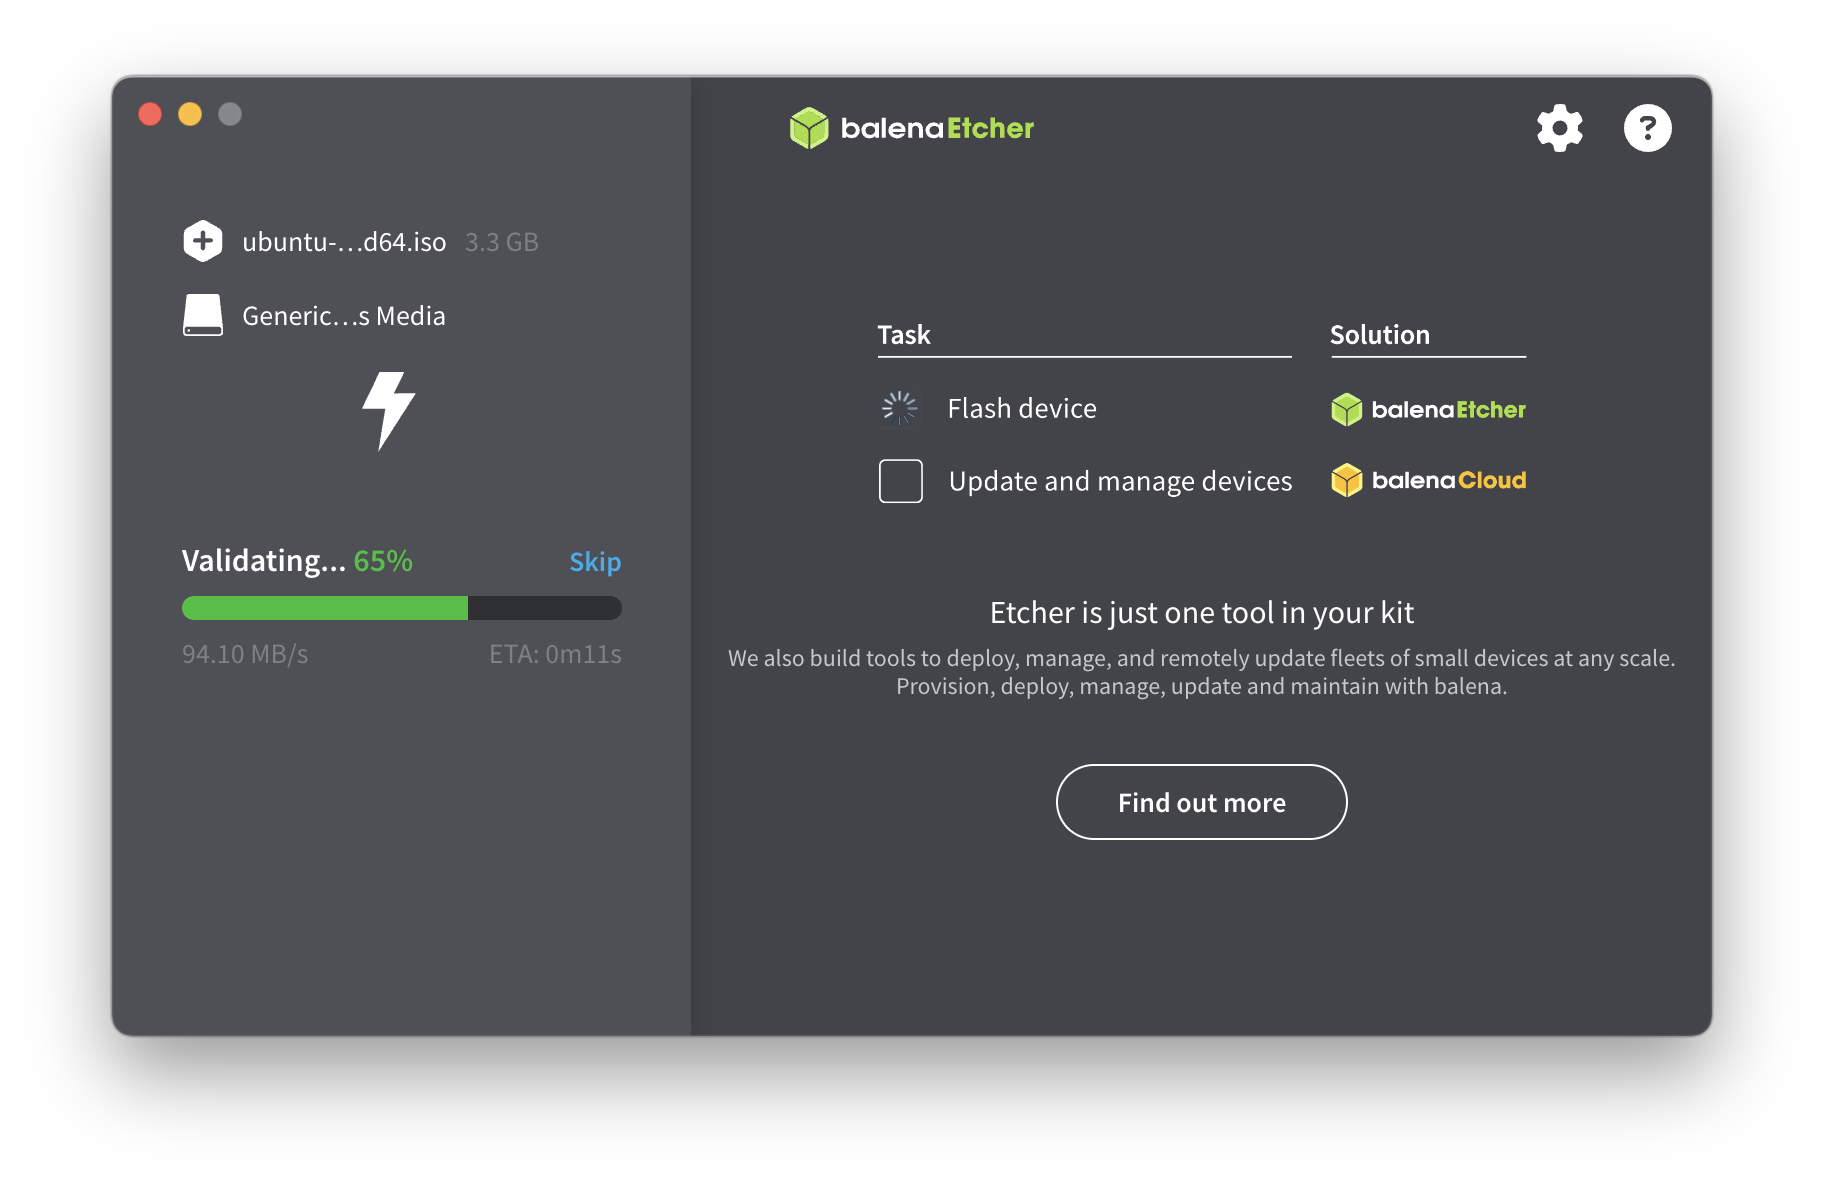
\includegraphics[width=.9\linewidth]{Install_Images/os-balenaetcher-validate.png}
  \captionof{figure}{Balena Etcher validating the written image to ensure data integrity.}
  \label{fig:balena2}
\end{minipage}
\end{figure}

\begin{figure}[H]
\centering
\begin{minipage}{.48\textwidth}
  \centering
  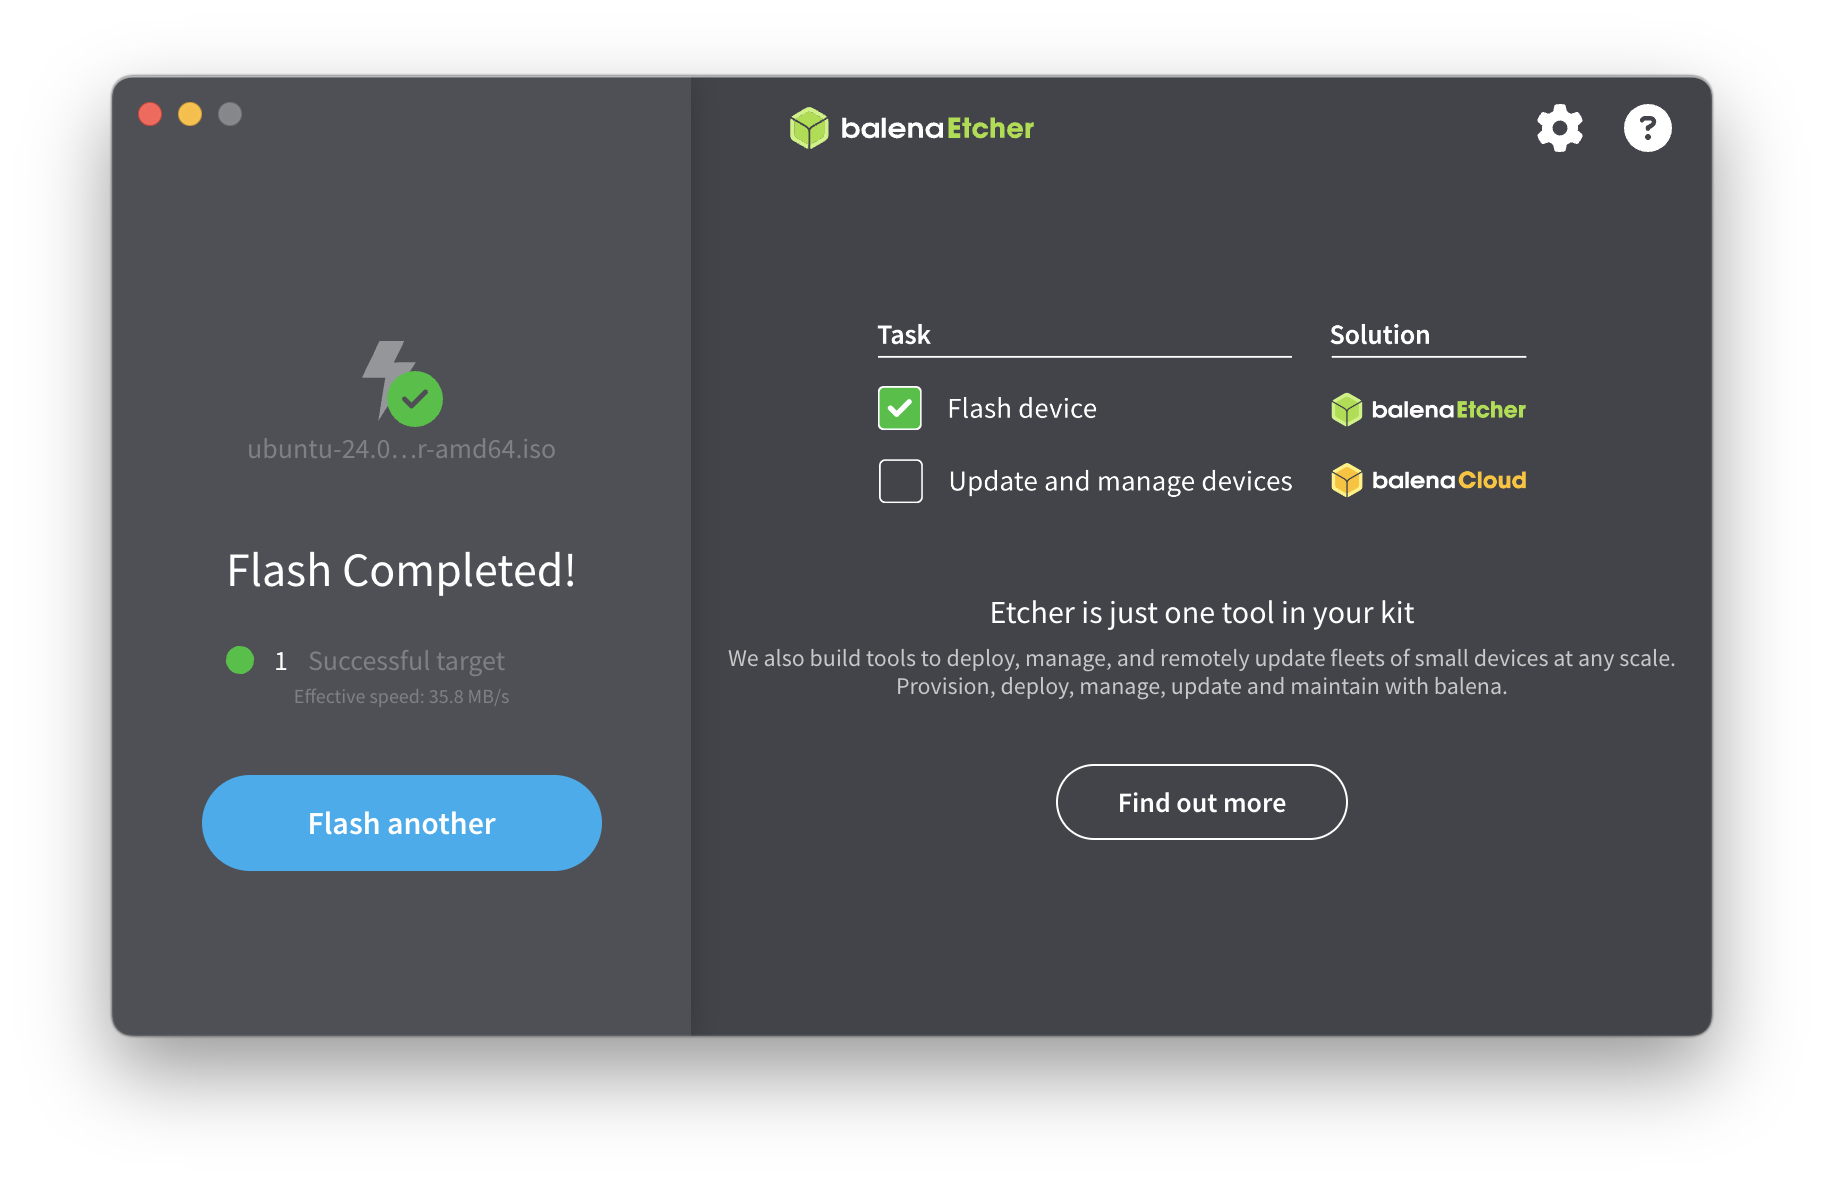
\includegraphics[width=.9\linewidth]{Install_Images/os-balenaetcher-finished.png}
  \captionof{figure}{Balena Etcher reporting successful completion of the flash operation.}
  \label{fig:balena3}
\end{minipage}\hfill
\begin{minipage}{.48\textwidth}
  \centering
  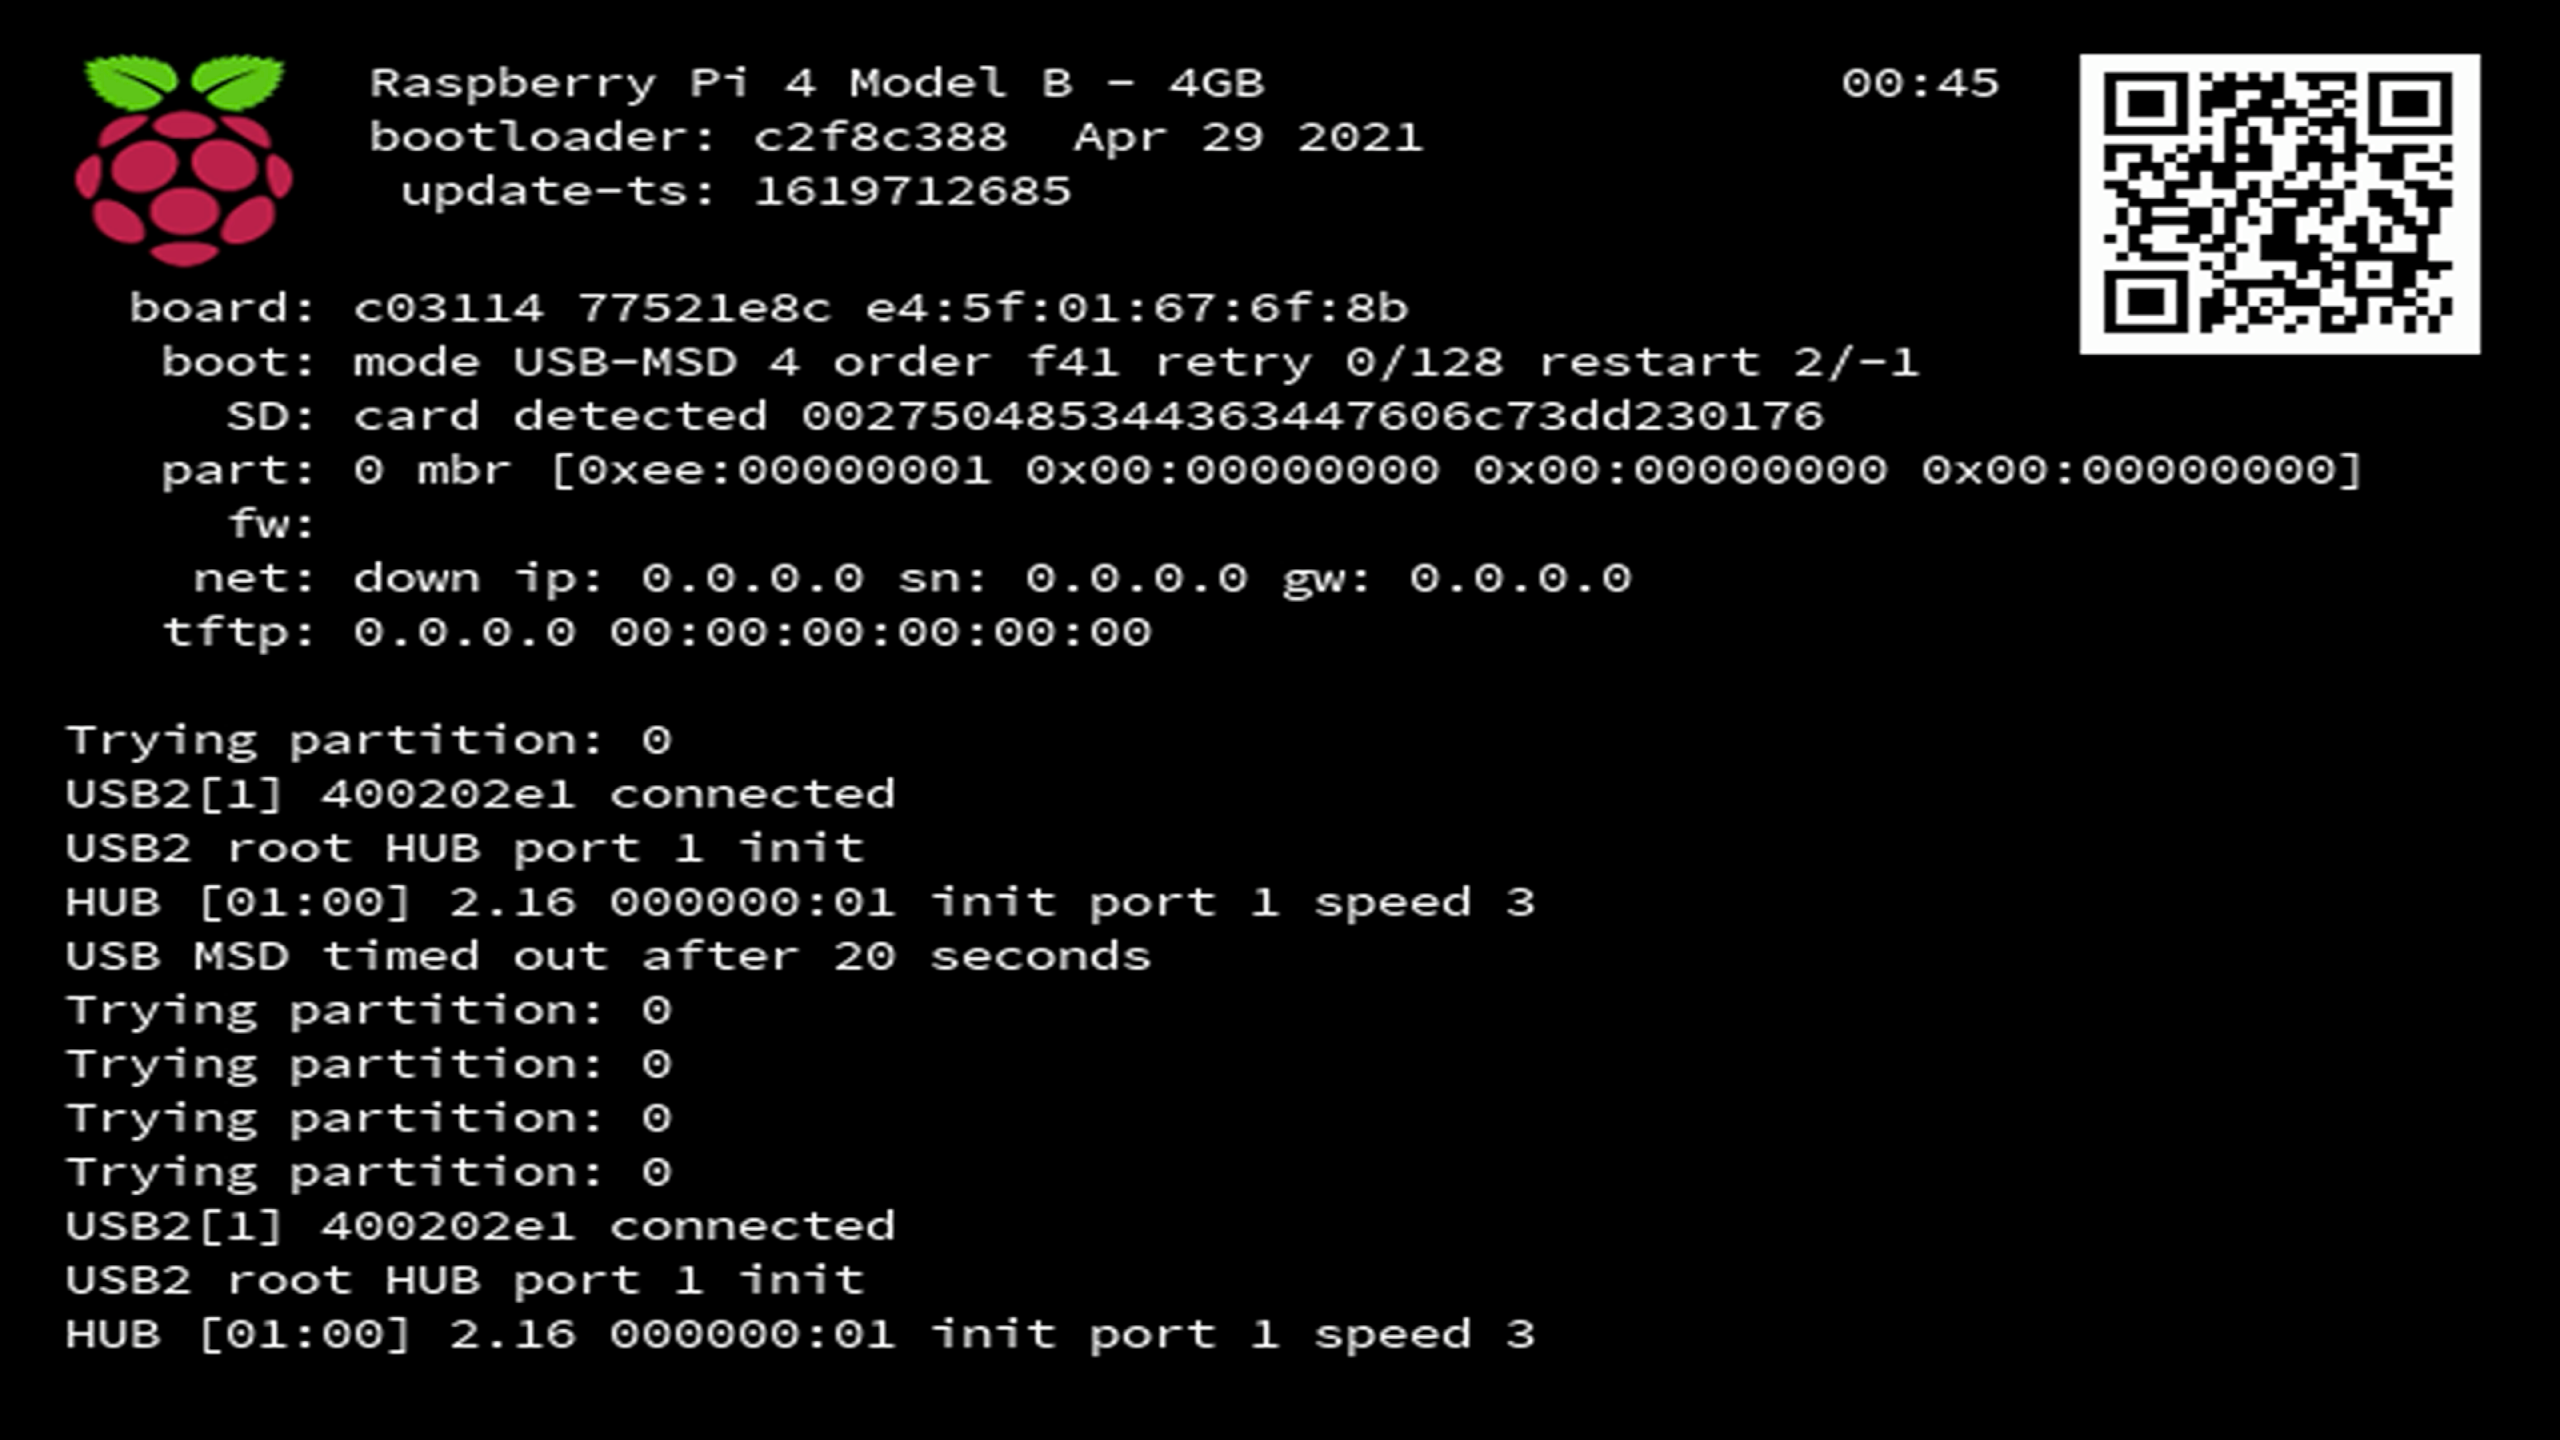
\includegraphics[width=.9\linewidth]{Install_Images/os-balenaetcher-fail-bootloader.png}
  \captionof{figure}{Raspberry Pi 4 bootloader failure}
  \label{fig:balena4}
\end{minipage}
\end{figure}

However, when I installed the SD card into the Raspberry Pi and powered it on, the system failed to boot successfully. Figure \ref{fig:balena4} shows the bootloader, not something you want to see. The error messages show:
\begin{itemize}
    \item \texttt{USB MSD timed out after 20 seconds} - The bootloader tried to read from the SD card but went past the timeout threshold
    \item \texttt{Trying partition: 0} - The bootloader detected no valid bootable partitions on the SD card
\end{itemize}

The boot failure highlights the firmware compatibility between the operating system image and the device's bootloader. Unlike traditional x86 BIOS/UEFI-based computers that follow a standardised boot spec, ARM-based SBCs sometimes need vendor-specific boot configurations like the Raspberry Pi Imager \parencite{RaspberryPi2024Imager}.

\subsubsection{Install - Raspberry Pi Imager}
\label{subsubsec:balena-install}
Following the balenaEtcher failure, I reattempted the install using the Raspberry Pi Imager \parencite{RaspberryPi2024Imager}. Unlike balenaEtcher (a generic disk imager), the Raspberry Pi Imager is purpose-built for Raspberry Pi hardware and automatically applies board-specific boot configurations, firmware updates, and more importantly, first-boot customisation options, so you can run the Pi over a local network (configuring an SSH server, credentials and providing hard-coded network information). Figure \ref{fig:install-base} shows the Raspberry Pi Imager interface with the device model (Raspberry Pi 4), operating system (Ubuntu Server 24.04 LTS 64-bit), and storage medium (SD card) selected.

\begin{figure}[H]
    \centering
    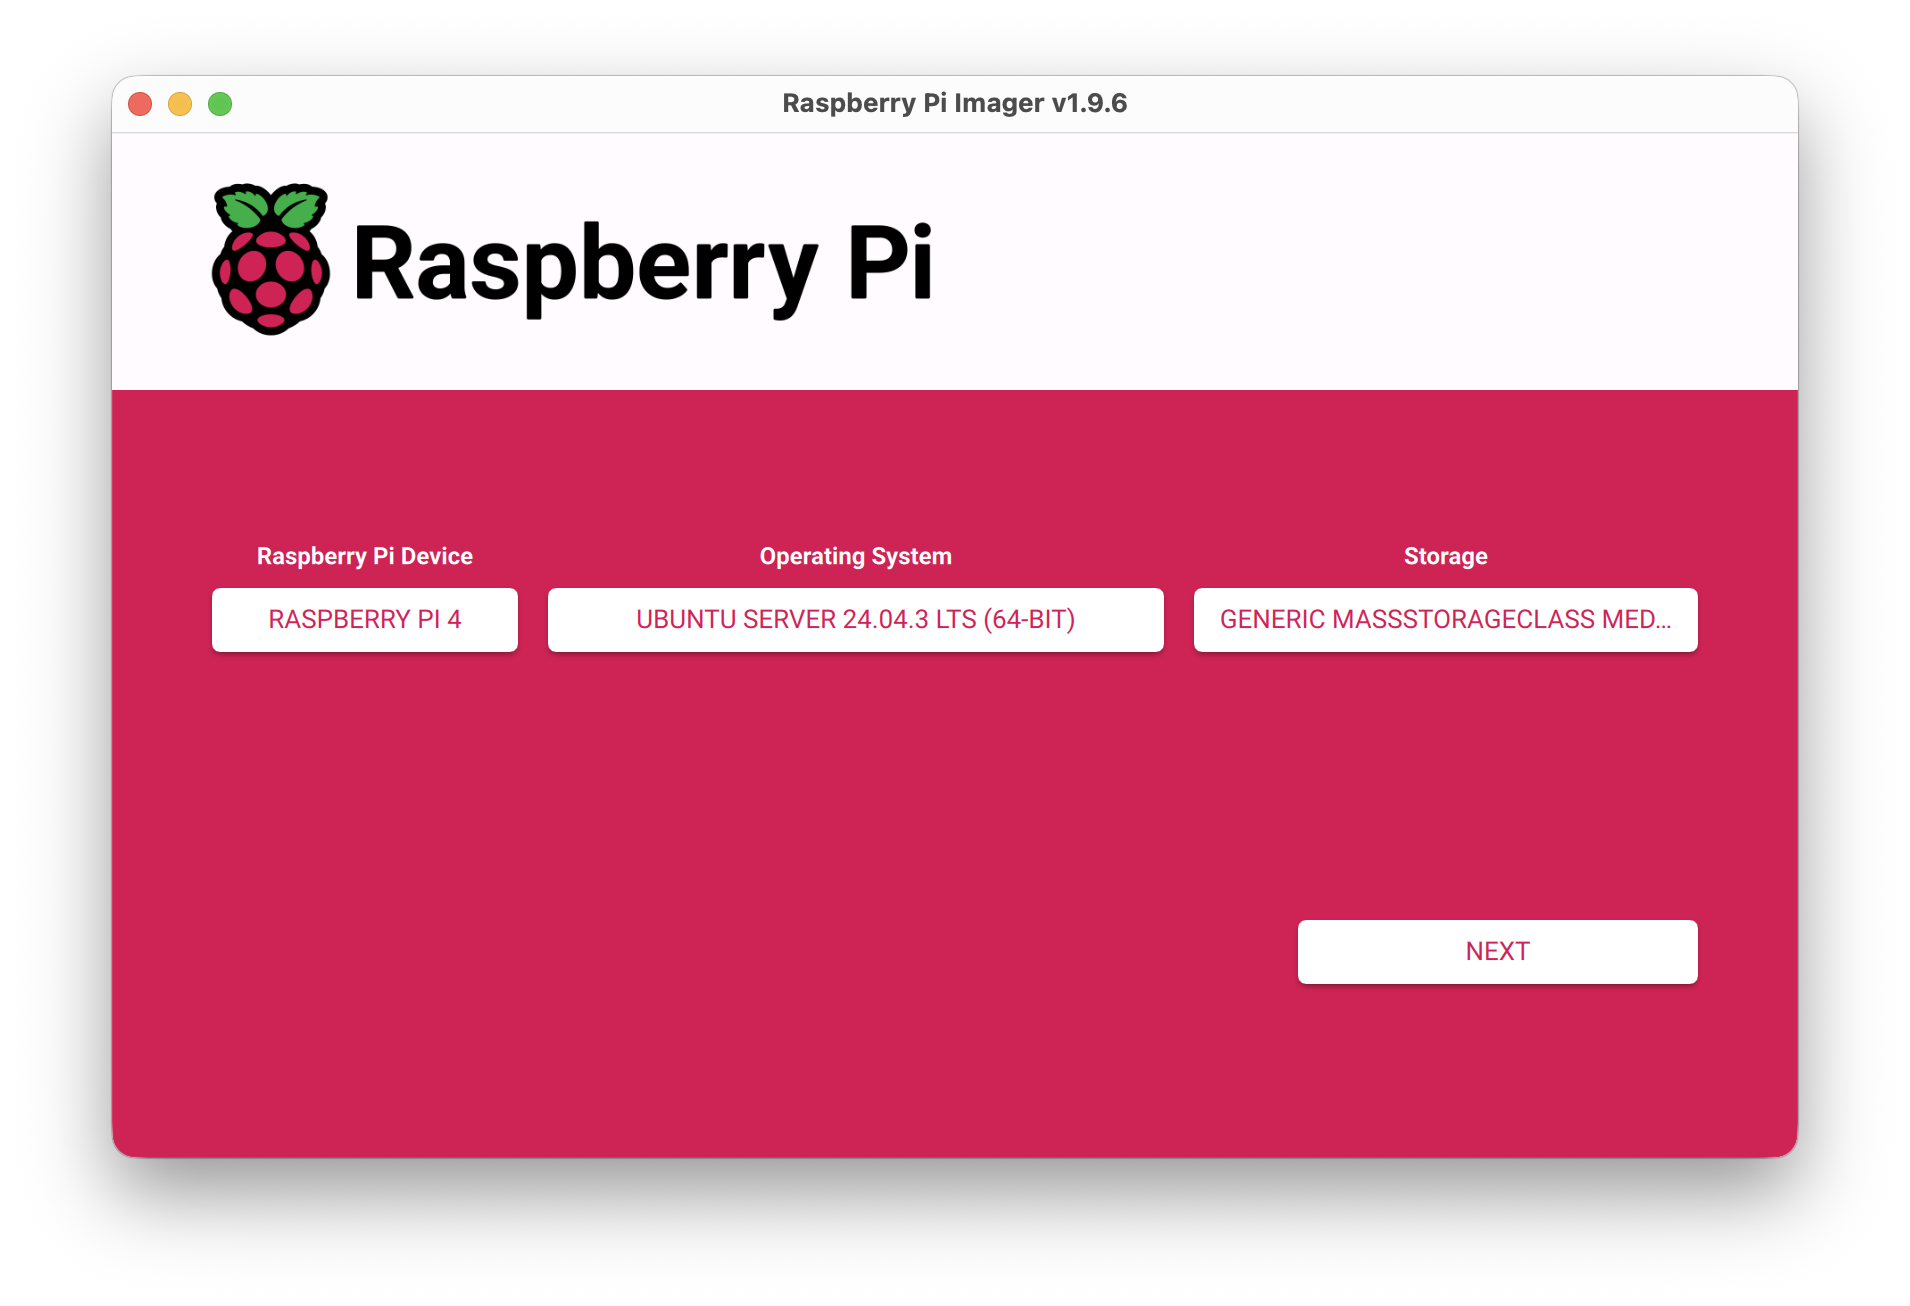
\includegraphics[width=0.7\linewidth]{Install_Images/os-raspi-imager-setup.png}
    \caption{Raspberry Pi Imager main interface showing device, OS, and storage selection before customization.}
    \label{fig:raspi-setup}
\end{figure}

Before writing the image, the Imager prompted for OS customization settings (Figure \ref{fig:raspi-extra-select}), which enables headless deployment without requiring physical access to the Raspberry Pi for initial configuration.

\begin{figure}[H]
\centering
\begin{minipage}{.48\textwidth}
  \centering
  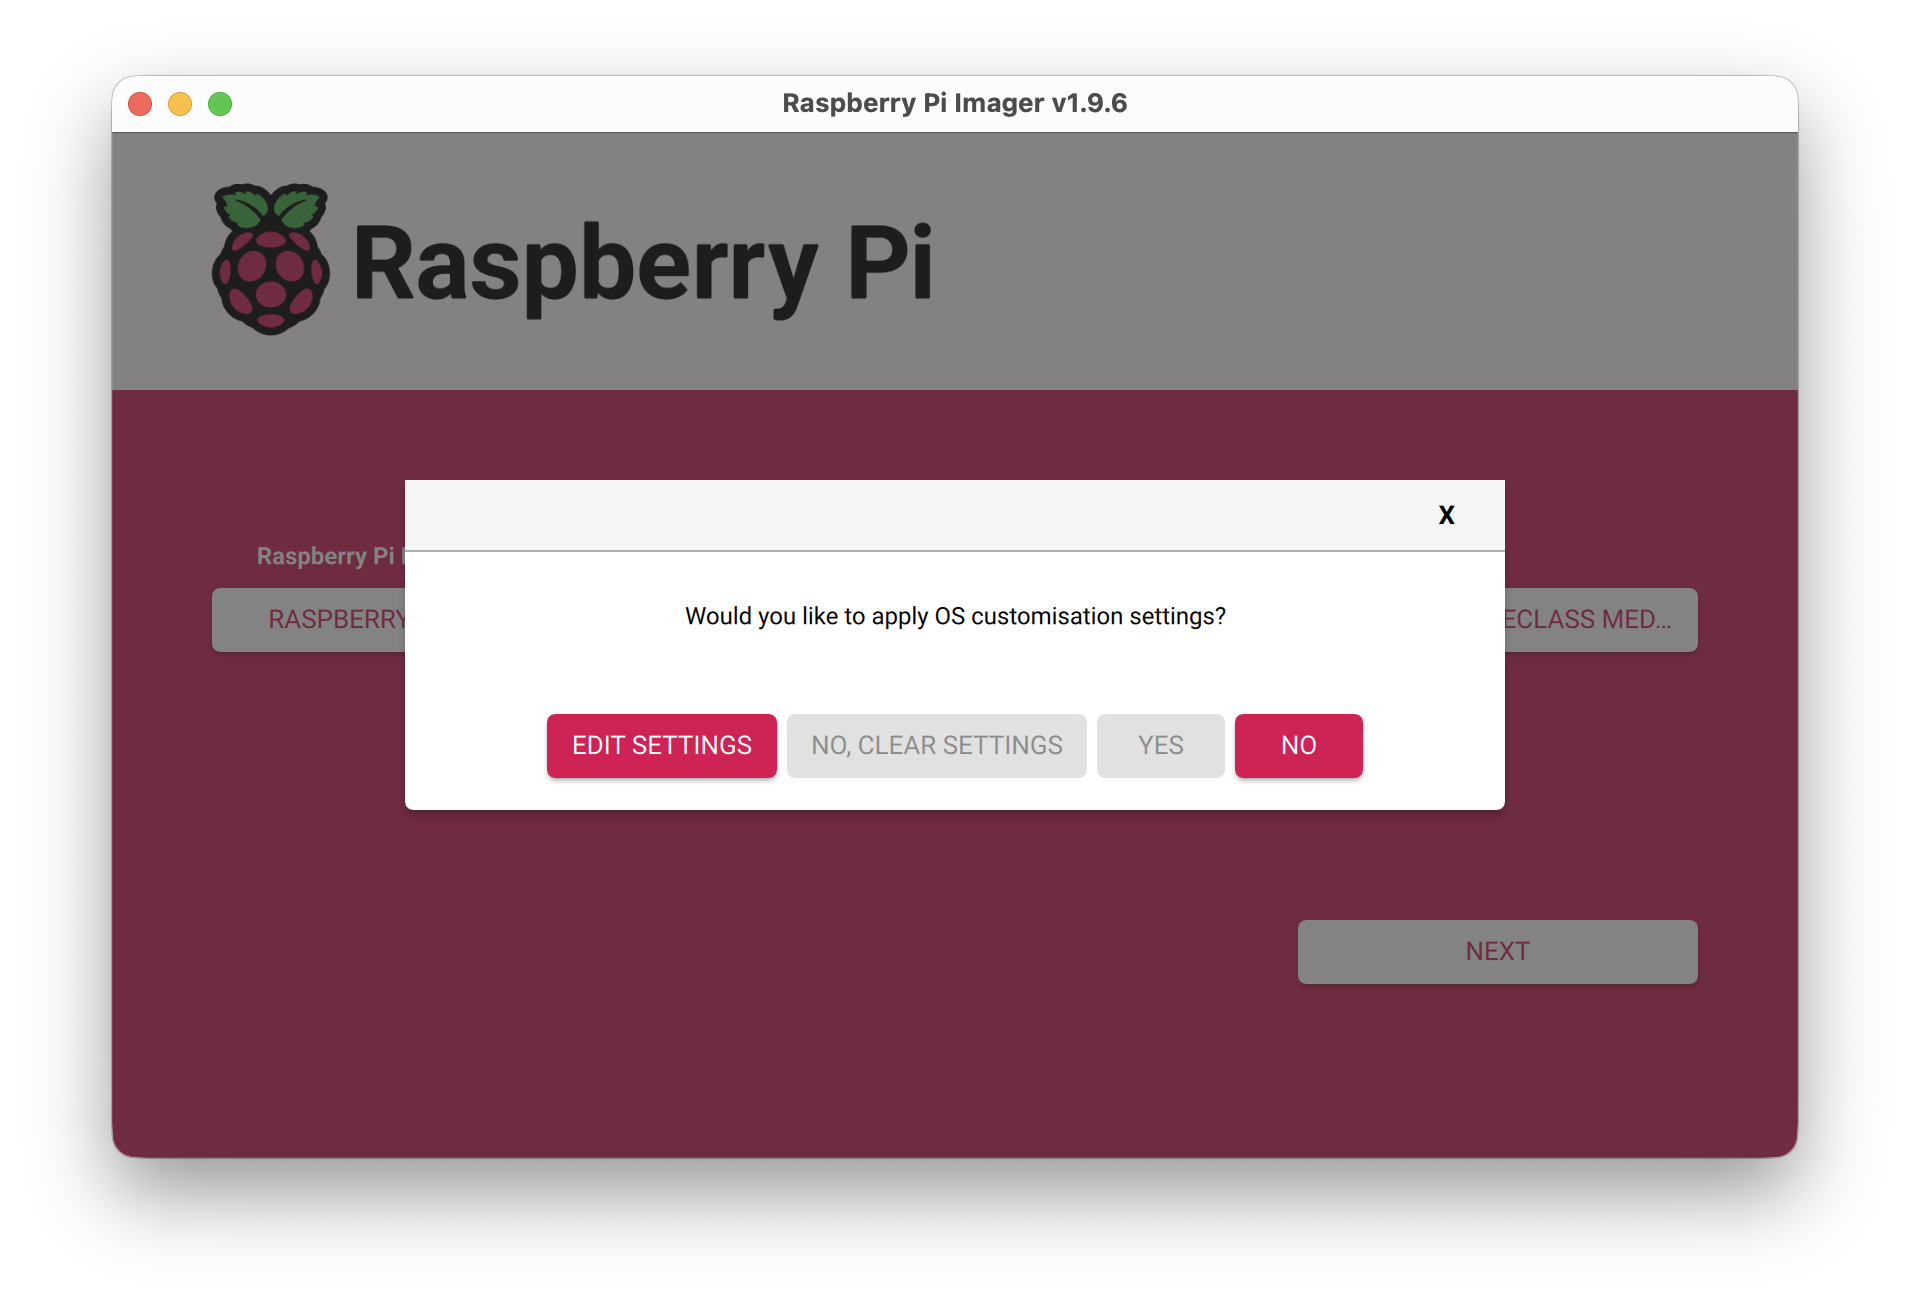
\includegraphics[width=.9\linewidth]{Install_Images/os-raspi-imager-extra-select.png}
  \captionof{figure}{OS customization prompt offering pre-boot configuration options.}
  \label{fig:raspi-extra-select}
\end{minipage}\hfill
\begin{minipage}{.48\textwidth}
  \centering
  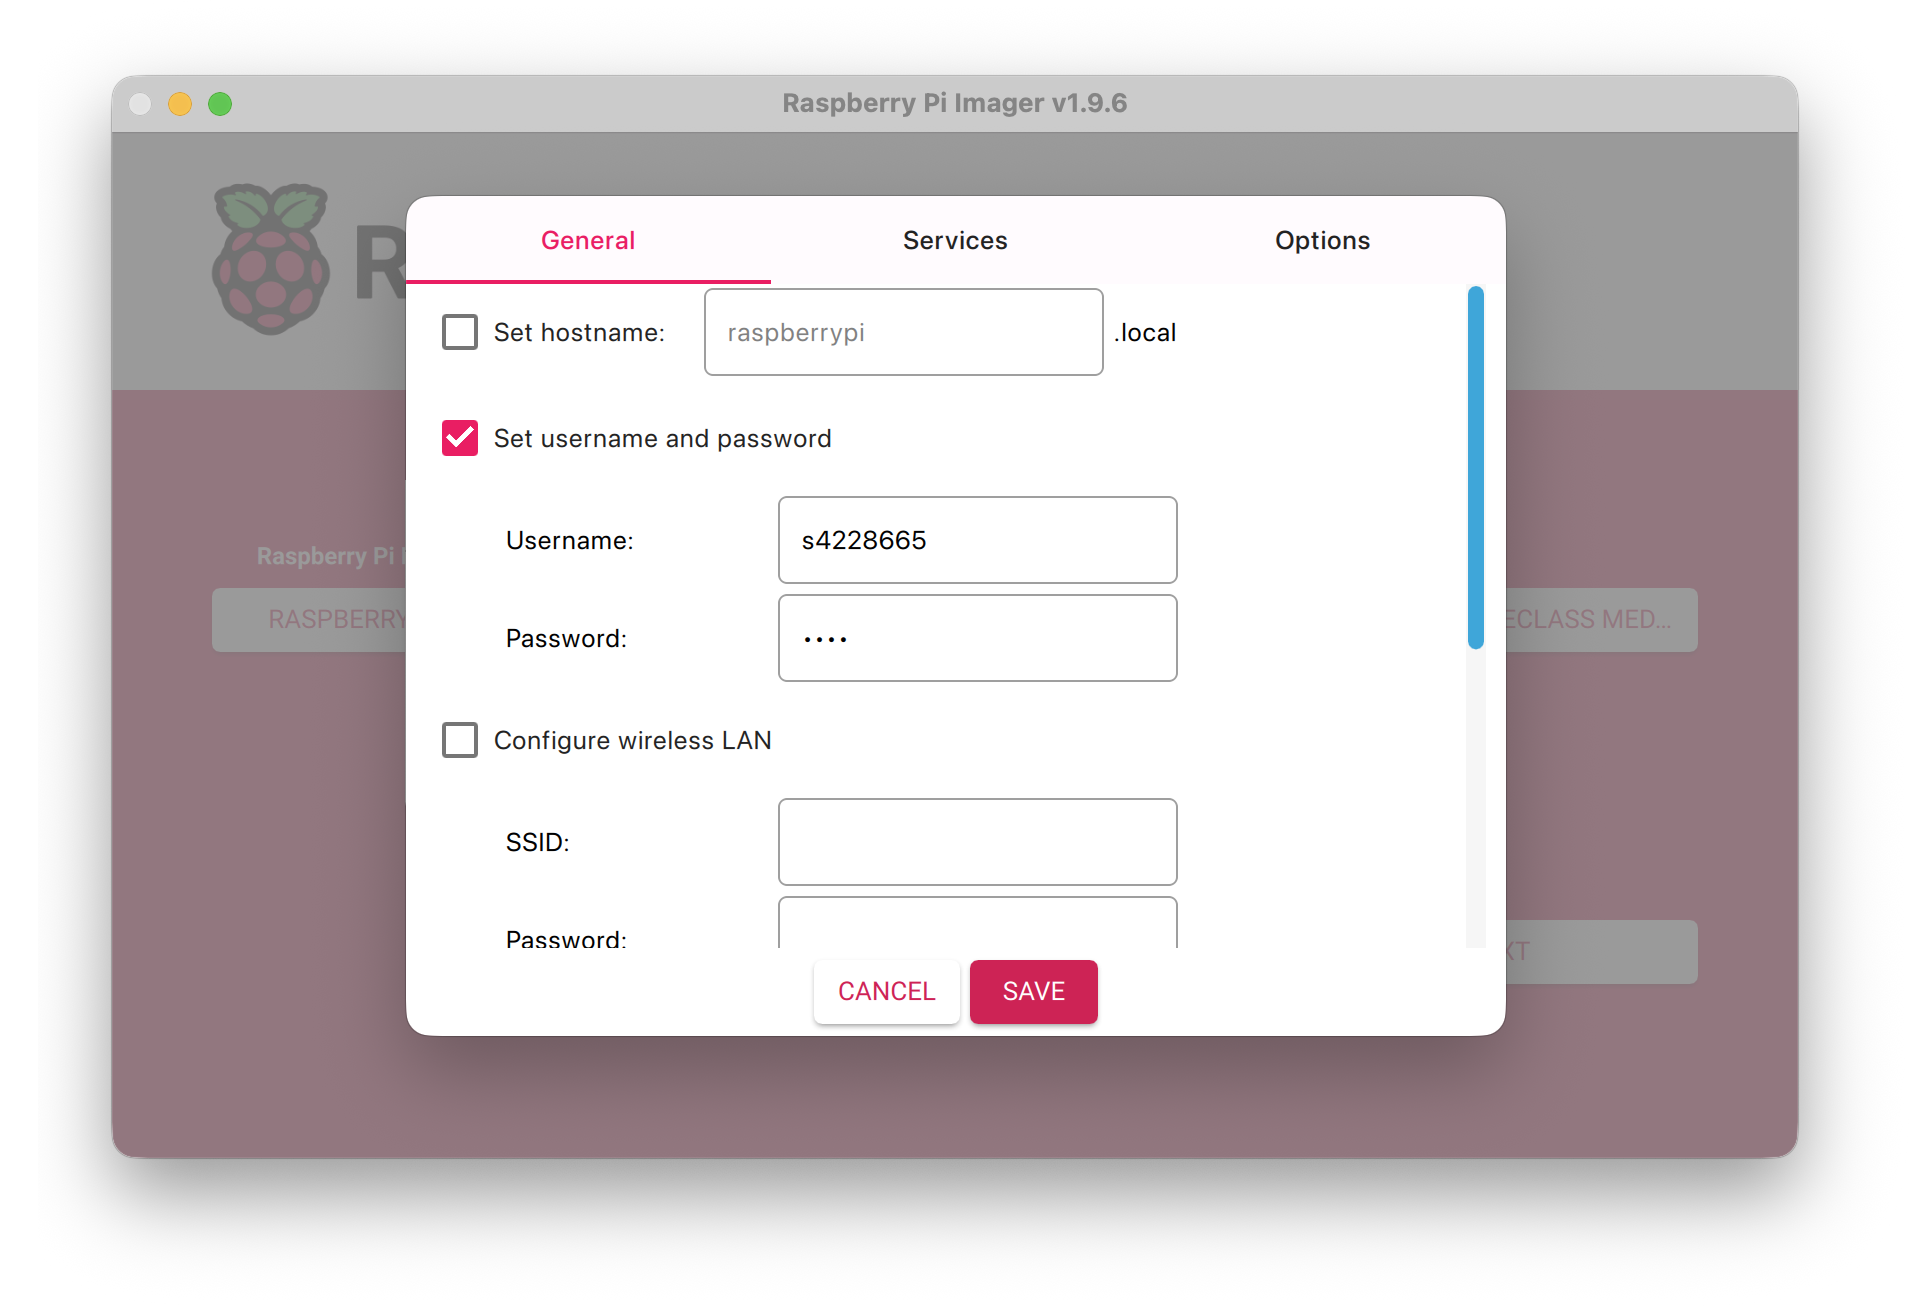
\includegraphics[width=.9\linewidth]{Install_Images/os-raspi-imager-extra.png}
  \captionof{figure}{Customization dialog showing my username (s4228665)}
  \label{fig:raspi-extra}
\end{minipage}
\end{figure}

The OS customisation fields (Figure \ref{fig:raspi-extra}) show I configured:
\begin{itemize}
    \item \textbf{Username}: \texttt{s4228665} (my student ID)
    \item \textbf{Hostname}: \texttt{raspberrypi.local} - left as default so it can be provisioned by Ansible (section \ref{sec:provision.yml})
    \item \textbf{Wireless LAN}: SSID and password - also left as default so it can be provisioned by Ansible (section \ref{sec:netplan.yml})
\end{itemize}

After confirming settings, the Imager wrote the image to the SD card (Figure \ref{fig:raspi-writing}).

\begin{figure}[H]
    \centering
    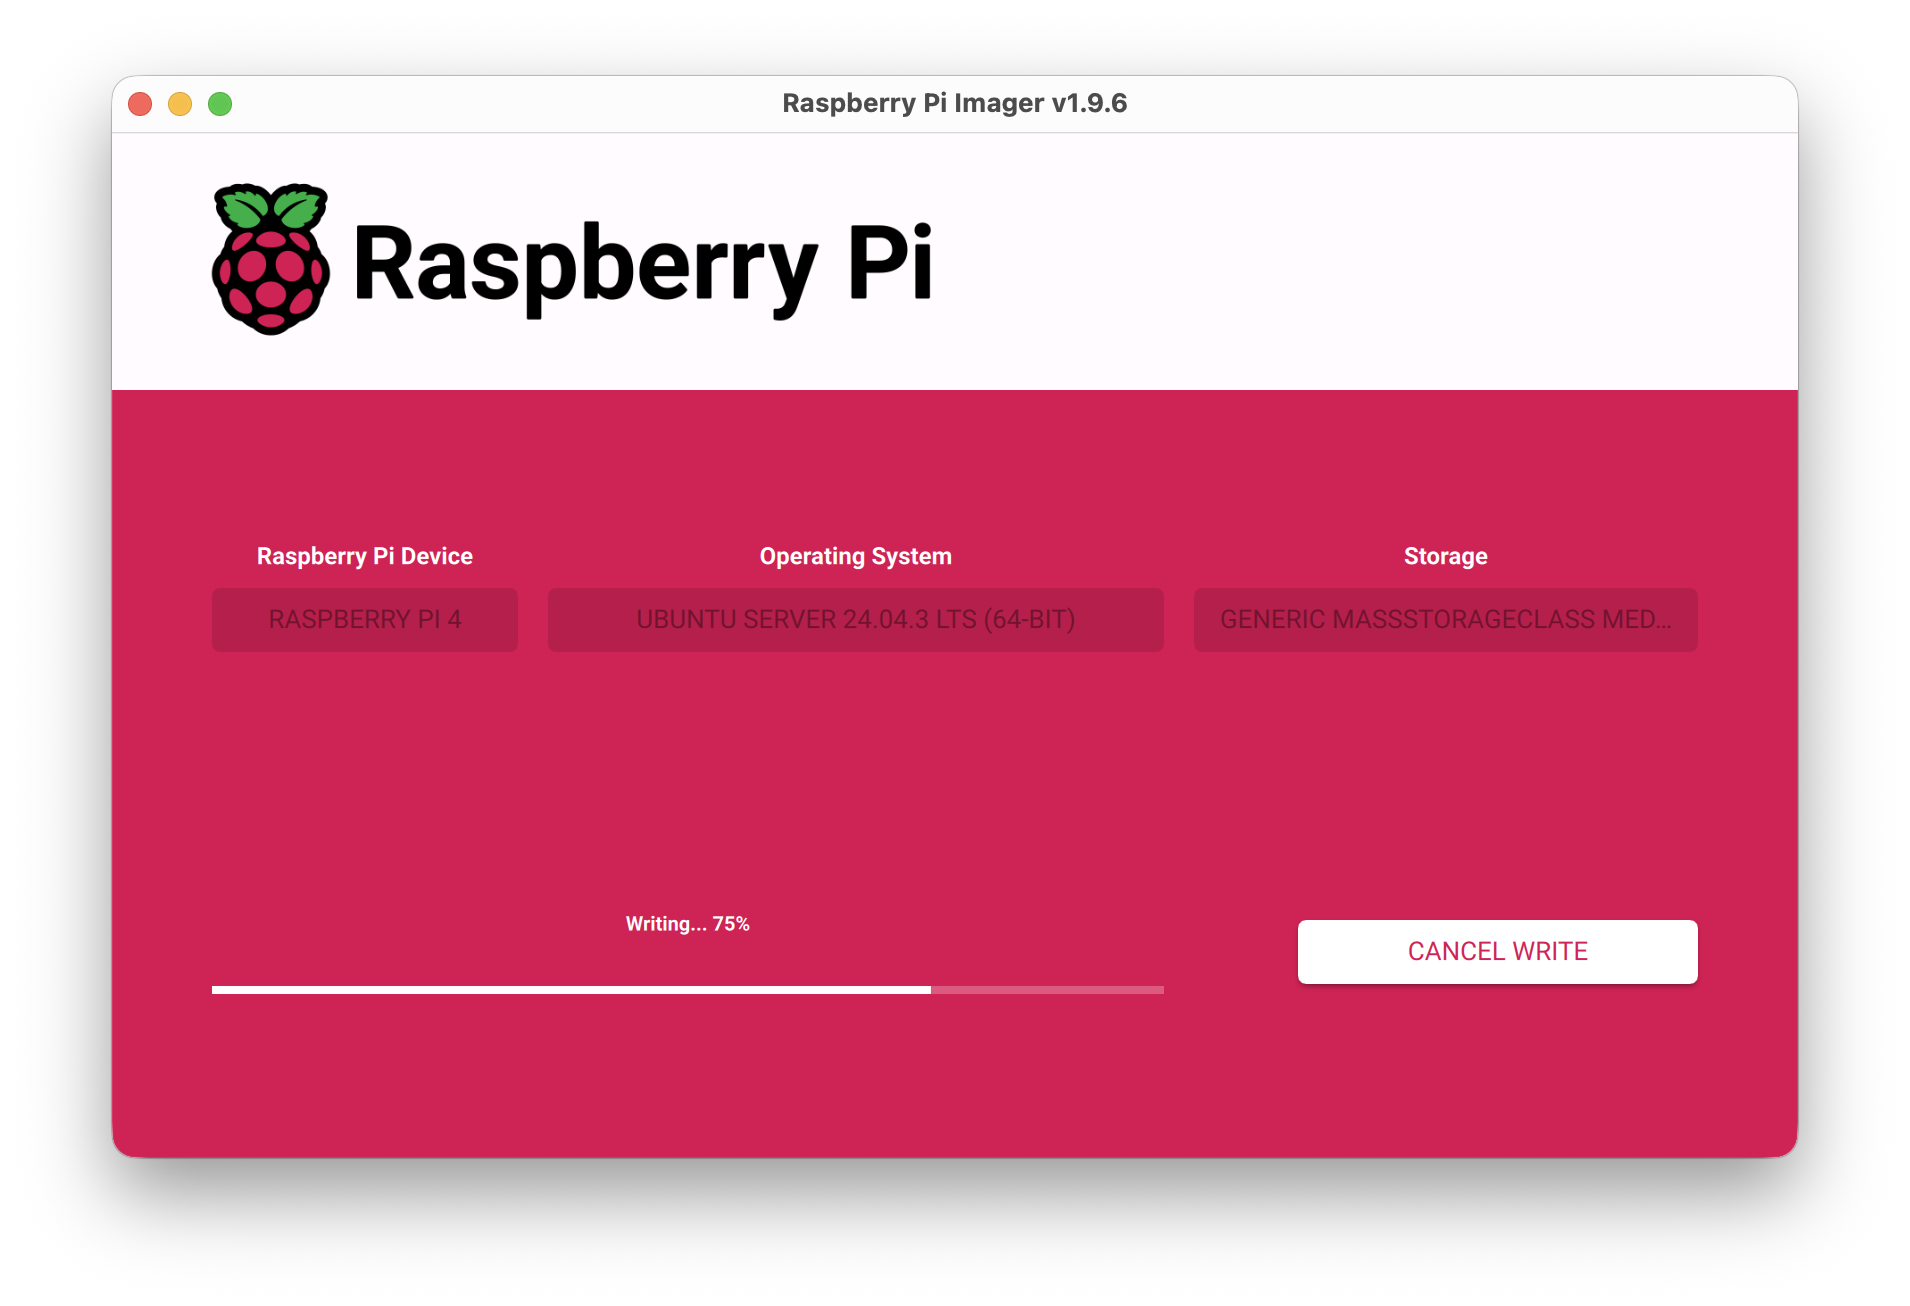
\includegraphics[width=0.7\linewidth]{Install_Images/os-raspi-imager-writing.png}
    \caption{The Imager at 75\% progress}
    \label{fig:raspi-writing}
\end{figure}

\subsubsection{First Boot and Initial Configuration}
\label{subsubsec:first-boot}

After inserting the SD card and turning on the Pi, the system booted into the OS, then started generating SSH host keys and starting the OpenSSH server (Figure \ref{fig:firewall-ssh}). The cloud-init system applied the pre-configured settings, which would allow immediate SSH access.

Please know these next screenshots (figures \ref{fig:firewall-ssh}, \ref{fig:firewall-load} and \ref{fig:firewall-adduser})are taken directly from the Pi plugged into a monitor via a capture card, I did try to make them as readable as possible but there was no real way to get better screenshots before enabling SSH access.

\begin{figure}[H]
    \centering
    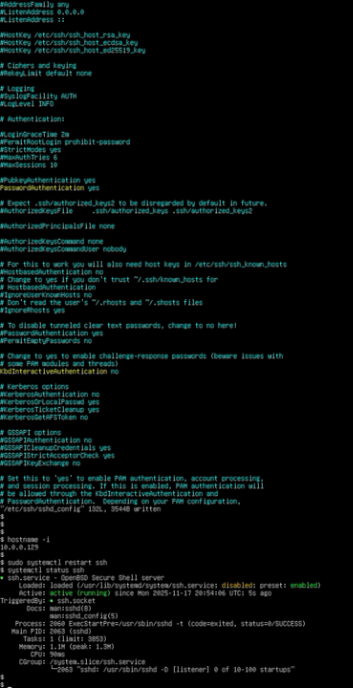
\includegraphics[width=0.5\linewidth]{Install_Images/os-firewall-ssh-config.png}
    \caption{First boot, followed by me setting up the OpenSSH server by changing the authentication config using VIM. As I didn't configure the IP config, the Pi has been assigned 10.0.0.125 via DHCP, ready for remote access}
    \label{fig:firewall-ssh}
\end{figure}

Figure \ref{fig:firewall-ssh} confirms:
\begin{itemize}
    \item The SSH service is active and running
    \item IPv4 address \texttt{10.0.0.125} assigned to \texttt{eth0} (onboard Ethernet interface)
    \item System fully accessible via SSH so screenshots can be take via a laptop and not a capture card
\end{itemize}

The base install of Ubuntu 24.04 (and other Ubuntu images) has a preconfigured Ubuntu user that, when you log in for the first time, the system asks you to change the password. If I had added my user in the additional settings page, this would not have been a problem. So when I logged in (Figure \ref{fig:firewall-load}) I changed the default user password. This practice shows Ubuntu's default security policy as it requires administrator-defined credentials instead of Ubuntu/Ubuntu.

\begin{figure}[H]
    \centering
    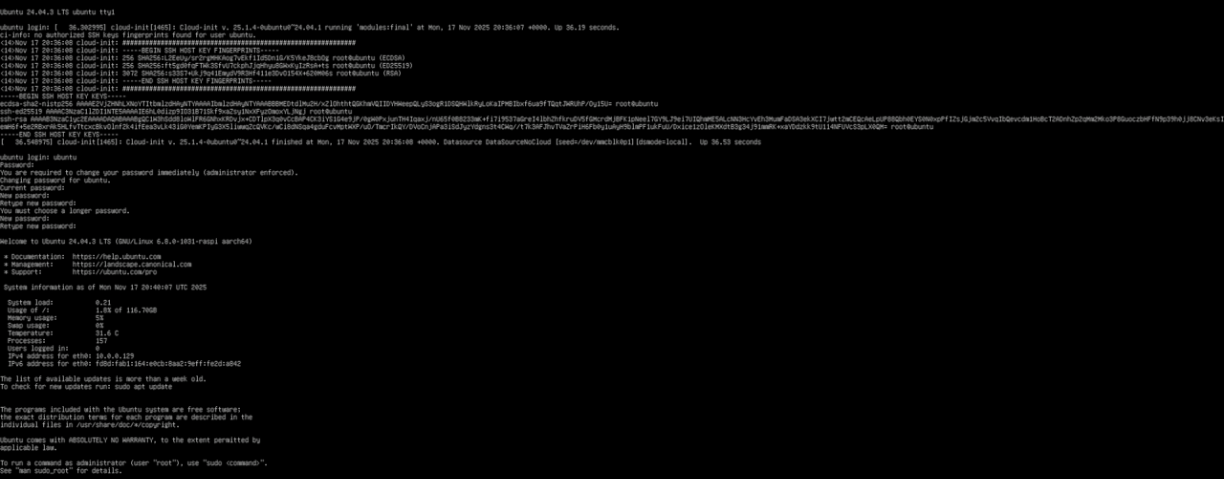
\includegraphics[width=0.95\linewidth]{Install_Images/os-firewall-load.png}
    \caption{Initial login showing mandatory password change prompt, system information (Ubuntu 24.04.3 LTS, Linux kernel 6.8.0-1051-raspi, 116.7MB memory usage), and available system updates notification.}
    \label{fig:firewall-load}
\end{figure}

Following the password change, I created my user (\texttt{s4228665}) and added myself to the sudoers file as I'll use this user to do ansible config deployments (figure \ref{fig:firewall-adduser}).

\begin{figure}[H]
    \centering
    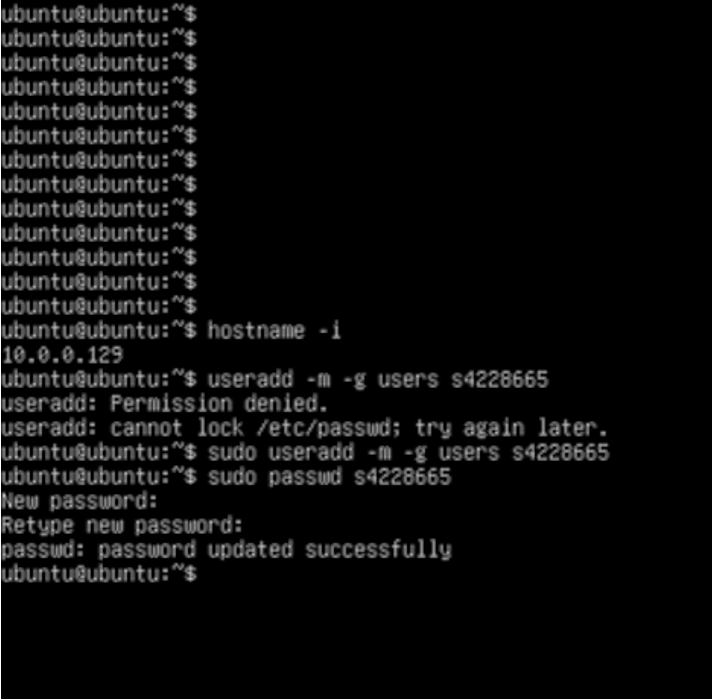
\includegraphics[width=0.95\linewidth]{Install_Images/os-firewall-add-user.png}
    \caption{Adding my user with \texttt{useradd} to create the (s4228665) user}
    \label{fig:firewall-adduser}
\end{figure}

In attempting to capture this process end-to-end elements were missed, the final step of getting my user configured and the OpenSSH server working took several tries until I was able to SSH from my laptop the first time (figure \ref{fig:firewall-first-ssh}), the main difference is when it finally worked DHCP from my local network assigned the Pi a final IP address of \verb|10.0.0.184|

\begin{figure}[H]
    \centering
    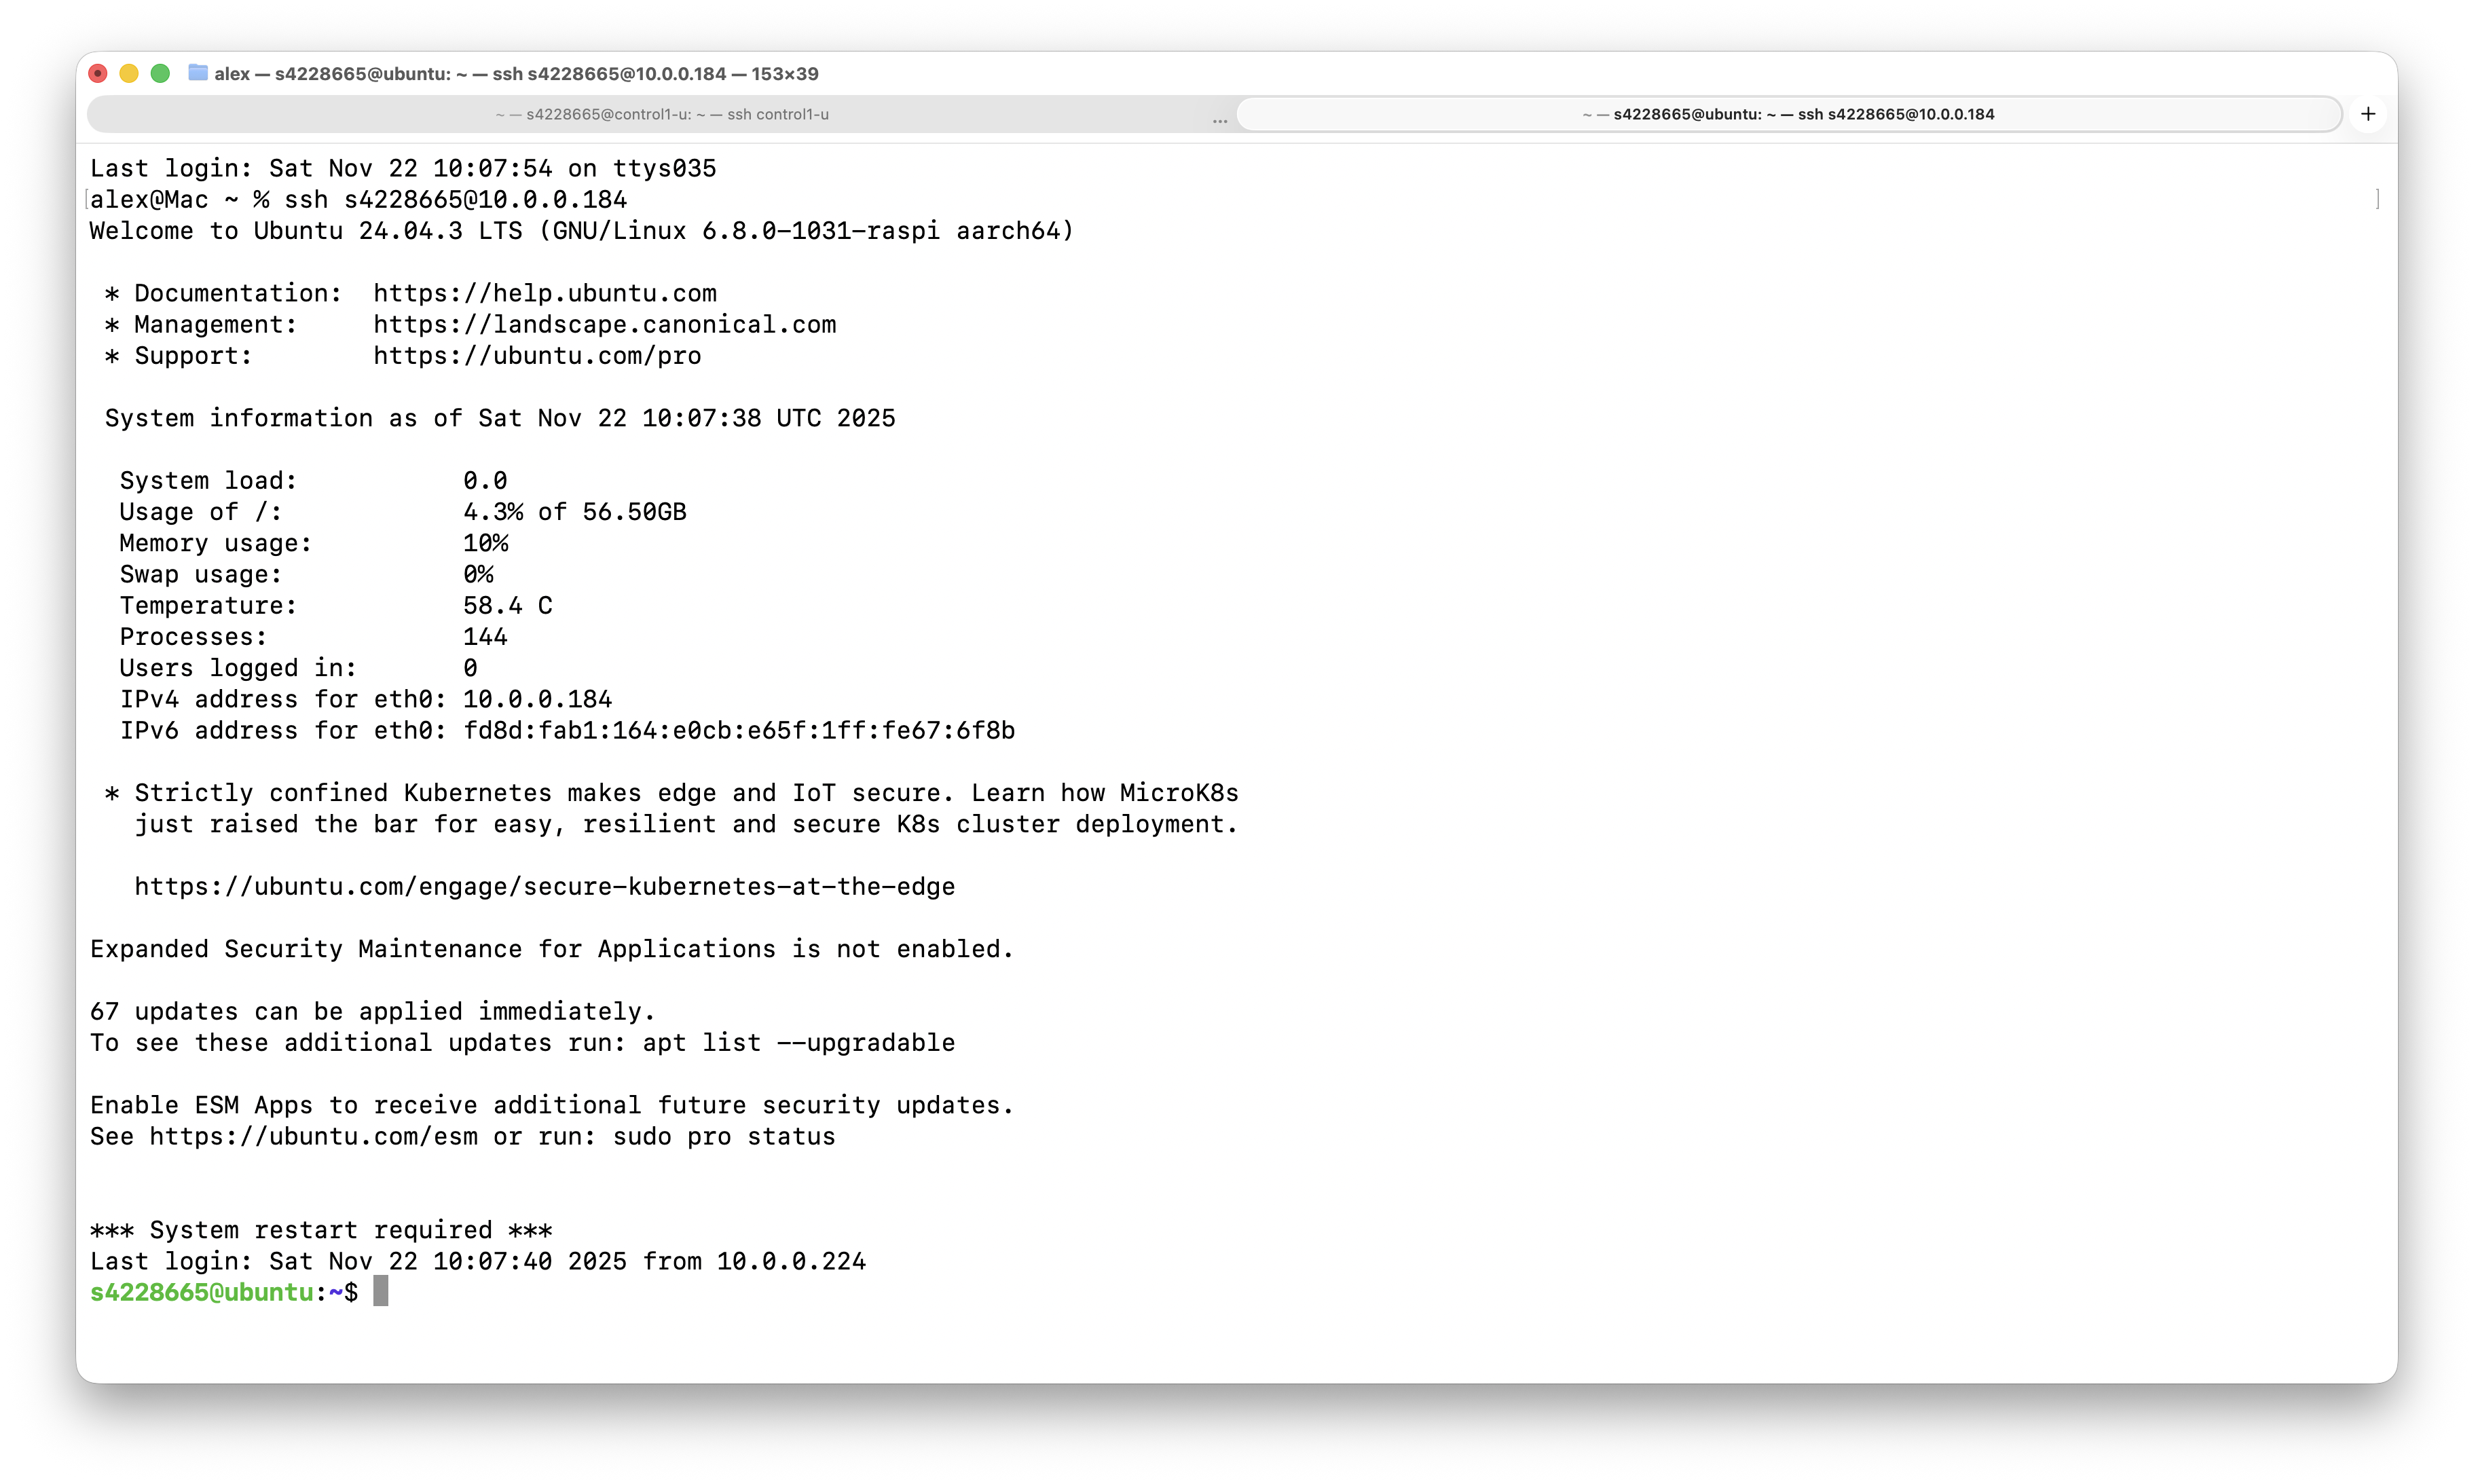
\includegraphics[width=0.95\linewidth]{Install_Images/os-alex-first-ssh.png}
    \caption{A successfull first SSH from my laptop}
    \label{fig:firewall-first-ssh}
\end{figure}
\subsection{Infrastructure as Code Approach}
\label{sec:IaC}
Infrastructure as Code (IaC) is a modern DevOps practice that enables the management and provisioning of infrastructure through code instead of manual processes, \parencite[]{RedHat2024InfrastructureAsCode} by using Ansible \parencite[]{RedHat2024Ansible} for configuration management and deployment, vagrant as a testing environment and storing all configuration in version control (github) this is achieved, mocking industry standard production and testing environments.

\subsubsection{Version control (VCS)}
As previously mentioned all configuration files, playbooks and templates are stored in a personal github repository \parencite{ErcModel3_2024OperatingSystems} so the project has:
\begin{itemize}
    \item Change tracking: every change has a valid commit message
    \item Rollback potential: if a mistake is made, I can go back within the repo's history and redeploy working config
    \item The potential for both group members to review/block code changes
    \item Up to date documentation for the state of the firewall
\end{itemize}

\subsubsection{Development workflow and Vagrant}
The coursework brief states that the "Implementation of the coursework should NOT be made on a virtual machine", but nothing about using virtual machines (VMs) for testing, as a real, industry environment would use. As such, using a Vagrant \parencite[]{HashiCorp2024Vagrant} defined VM to run an ARM64 Ubuntu 24.04 (using the net9/ubuntu-24.04-arm64 on an ARM-based dev machine and the ) box mirrored the environment of the 'production' Raspberry Pi (aside from the additional network interface (NIC)). This was defined as figure \ref{code:vagrant-vm-definition}. Vagrant was picked as the program to use as it works as an abstraction layer to define a virtual machine suited for the development environment. The Vagrantfile is Ruby-based, so I could have added automatic checks using Ruby to determine the CPU architecture as I switch between my PC (x86-based Windows/Ubuntu Machine) and my laptop (ARM-based MacBook Air) but I have opted for commenting each line out when it's not being used e.g. \verb|# rasta.vm.box = "net9/ubuntu-24.04-arm64"| when using the cloud (x86) image.

\begin{figure}[H]
    \centering
    \begin{minted}{Ruby}
Vagrant.configure("2") do |config|
    config.vm.define "firewall2-u" do |rasta|
      # rasta.vm.box = "net9/ubuntu-24.04-arm64"
      rasta.vm.box = "cloud-image/ubuntu-24.04"

      rasta.vm.network "private_network", ip: "10.0.1.185"

      rasta.vm.provider "virtualbox" do |v|
        v.memory = 4096
        v.cpus = 2
        v.name = "control1-vagrant"
      end

      rasta.vm.provision "ansible" do |ansible|
        ansible.playbook = "provision.yml"
        ansible.limit = "all"
      end
    end
  end
    \end{minted}
    \caption{The Vagrantfile defining the virtual machine 'firewall2-u' as a testing environment }
    \label{code:vagrant-vm-definition}
\end{figure}

This VM acts as [firewall-test] target in the Ansible inventory, while the physical Pi is the [firewall-prod] at IP 10.0.0.1 as per figure \ref{subsec:ansible}. Combining Ansible, Git(hub) and Vagrant ensures:
\begin{itemize}
    \item Safe experimentation: Any rules created can be tested before pushing them to the real Firewall
    \item Continuous Integration \parencite{IBM2024CICDPipeline}: as both students can push code to their respective VM
    \item Additional snapshots/rollbacks: VirtualBox snapshots allow instant restoration of the VM should bad config get pushed
\end{itemize}

This implementation follows the development flow of figure \ref{fig:dev-workflow}
\begin{figure}[H]
    \centering
    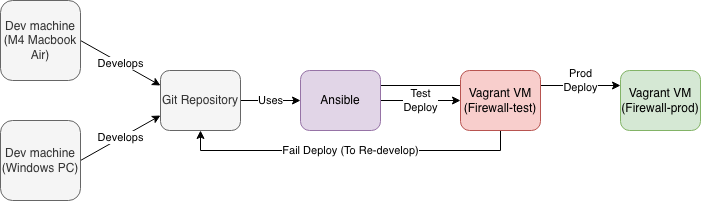
\includegraphics[width=0.8\linewidth]{Diagrams/os-dev-workflow.drawio.png}
    \caption{A diagram showing a high-level breakdown of the development workflow from dev machine to firewall instead of working just on the Pi and losing everything should a mistake arise}
    \label{fig:dev-workflow}
\end{figure}

\subsubsection{Configuration Management with Ansible}
Ansible is one of the most common open-source configuration management tools \parencite[]{OpenSource2018ConfigurationManagement}, it was selected as its:
\begin{itemize}
    \item Agentless: Less overhead on the Raspberry Pi as all work is done on the development machine and uses SSH to deploy files
    \item Idempotency: Playbooks can be run over and over and won't change anything unless there's a change to the codebase
    \item Comprised of easily-readable YAML playbooks
\end{itemize}

\paragraph{Playbook Structure - provision.yml}
\label{sec:provision.yml}
Each playbook/role has a definition and an endgoal. The \verb|provision.yml| playbook is attached to the \verb|vagrantfile| so it provisions the vm, it also provisions the Raspberry Pi.

NEEDS REFERENCE

\paragraph{Playbook Structure - netplan.yml}
\label{sec:netplan.yml}
To adhere to Ansible best practices \parencite{Ansible2024RoleReuse}, playbooks are all defined using the Role definition using a main YAML file that will call the role, figure \ref{code:ansible-netplan-role} shows the netplan role.

\begin{figure}[H]
    \centering
    \begin{minted}{YAML}

    \end{minted}
    \caption{The playbook used to deploy the netplan config to the test (and production) firewalls using Ansible facts}
    \label{code:ansible-netplan-role}
\end{figure}

\paragraph{Playbook Structure - iptables.yml}
\label{sec:iptables.yml}

TODO - REWRITE THIS PARAGRAPH
To adhere to Ansible best practices \parencite{Ansible2024RoleReuse}, playbooks are all defined using the Role definition using a main YAML file that will call the role.

\begin{figure}[H]
    \centering
    \begin{minted}{YAML}
---
- name: Install and deploy firewall
  hosts: firewall-test
  become: yes
  roles:
    - iptables
    \end{minted}
    \caption{The playbook used to deploy the Iptables config to the test (and production) firewall}
    \label{code:ansible-iptables-role}
\end{figure}

\begin{figure}[H]
    \centering
    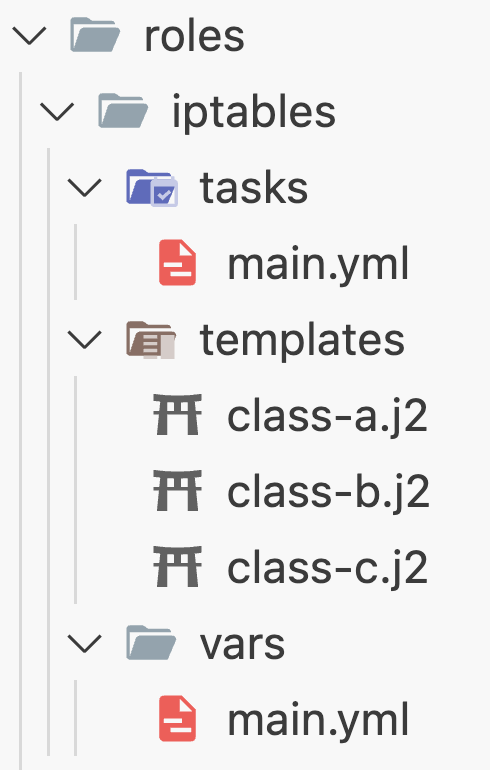
\includegraphics[width=0.3\linewidth]{Report_Images/os-iptables-role.png}
    \caption{The iptables Ansible role structure following best-practice}
    \label{screenshot:ansible-iptables-role}
\end{figure}

The main playbook (iptables.yml shown in figure \ref{code:ansible-iptables-role}) sets up and deploys the config to the testing firewall and the production firewall (when 'test' is substituted with 'prod'). Figure \ref{screenshot:ansible-iptables-role} shows the rest of the role the \verb|iptables.yml| playbook calls, namely the tasks file in \verb|tasks/main.yml| file in figure \ref{code:ansible-iptables-tasks}.

\begin{figure}[H]
    \centering
    \begin{minted}{YAML}
---
- name: Install iptables-persistent
  apt:
    name:
      - iptables-persistent
    update_cache: yes

- name: Create config directory
  file:
    dest: /etc/iptables/
    state: directory
    mode: '0664'

- name: Deploy iptables configs
  template:
    src: "{{ item }}.j2"
    dest: /etc/iptables/{{ item }}
  loop:
    - class-a
    - class-b
    - class-c
  
- name: Apply iptables configs
  command: iptables-save > {{ item }}
    \end{minted}
    \caption{The tasks file used to carry out the iptables deployment}
    \label{code:ansible-iptables-tasks}
\end{figure}

The tasks file:
\begin{itemize}
    \item Installs iptables-persistent package
    \item Creates the /etc/iptables directory
    \item Renders a Jinja2 template for each network zone as defined in \ref{} TO DO REFERENCE.
\end{itemize}
\subsection{Network Configuration}
\label{subsec:network-config}
As touched on when discussing netplan (section \ref{sec:netplan.yml}) \parencite{Ubuntu2024NetplanDesign} the 3 NICs must be configured with the correct IP addressing scheme and networks. Figure \ref{fig:basic-fw-breakdown} shows a high-level breakdown of the firewall zones and NICs, each for a different usecase and level of security. This config is deployed via Ansible for consistency and to adhere to the DevOps practices mentioned in section \ref{sec:IaC}. The networks should be manually assigned to allow for some level of persistence, the firewall as the gateway for each internal zone:

\begin{table}[H]
\centering
\begin{tabular}{|l|l|l|l|}
\hline
\textbf{Zone} & \textbf{Interface} & \textbf{Network} & \textbf{Firewall IP} \\ \hline
WAN (Internet) & eth0 & 10.0.0.0/8 & 10.0.0.5/8 \\ \hline
LAN (Trusted) & eth1 & 172.16.0.0/16 & 172.16.0.1/16 \\ \hline
Guest (IoT) & eth2 & 192.168.0.0/24 & 192.168.0.1/24 \\ \hline
\end{tabular}
\caption{IP addressing for each firewall zone}
\label{tab:ip-addressing}
\end{table}

The netplan role structure follows Ansible best practices:

\begin{verbatim}
roles/netplan/
├── tasks/main.yml          # Deployment tasks
├── templates/netplan.j2     # Jinja2 netplan template
├── vars/main.yml           # Network configuration variables
└── handlers/main.yml       # Netplan apply handler
\end{verbatim}

Figure \ref{fig:netplan-tasks} shows the Ansible task list that disables Ubuntu's cloud-init network management (which conflicts with static configuration) and deploys the templated netplan configuration file.

\begin{figure}[H]
    \centering
    \begin{minted}{YAML}
    Hello
    \end{minted}
    \caption{The playbook used to deploy the Iptables config to the test (and production) firewall}
    \label{code:ansible-neplan-tasks}
\end{figure}

The first task creates a new cloud-init file that stops Ubuntu from creating / using it's own network configuration and preventing cloud-init from reverting back on subsequent boots. The second task deploys the Jinja2-templated netplan configuration to \texttt{/etc/netplan/50-cloud-init.yaml}, creating a backup of any existing configuration before overwriting.

\begin{figure}[H]
    \centering
    \begin{minted}{YAML}
    Hey there
    \end{minted}
    \caption{The handlers used for the netplan role}
    \label{code:ansible-neplan-handlers}
\end{figure}

Both tasks trigger the \texttt{netplan apply} handler (Figure \ref{code:ansible-neplan-handlers}), which applies the new netplan config without needing a system reboot.


\subsubsection{Installing NIC drivers}
The coursework provides an additional NIC so this firewall is able to accommodate all 3 zones at the same time. To determine the type of NIC I was given I checked the connected usb devices and picked the appropriate entry provided in the VLE (figure \ref{fig:command-lsusb} and driver \parencite{Morrownr2024_8812au_Driver})

\begin{figure}[H]
    \centering
    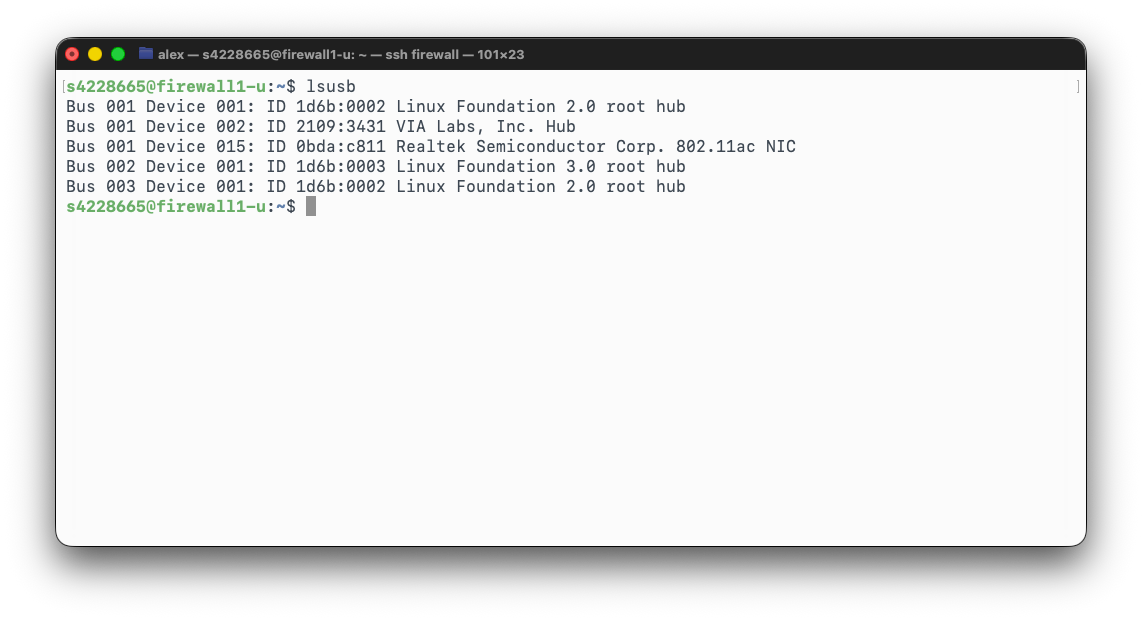
\includegraphics[width=0.8\linewidth]{Screenshots/command-lsusb.png}
    \caption{Enter Caption}
    \label{fig:command-lsusb}
\end{figure}

To install the driver I followed the steps from the repo \parencite{Morrownr2024_8812au_Driver} and collapsed them into a playbook called \verb|provision.yml| \ref{code:ansible-provision-playbook}. This playbook provisions both the test environment and the production firewall, only running certain plays on certain hosts (e.g. my user will already be on the Pi but not a newly made test environment).

\begin{figure}[H]
    \centering
    \begin{minted}{YAML}
    I'm the strongest dude
    \end{minted}
    \caption{The handlers used for the netplan role}
    \label{code:ansible-provision-playbook}
\end{figure}

We can test this by running the playbook via vagrant using \verb|vagrant up| when the playbook is referenced in the \verb|vagrantfile|, the output for this can be seen in figure \ref{vagrant:provision-vm-nic}.

\begin{figure}[H]
    \centering
    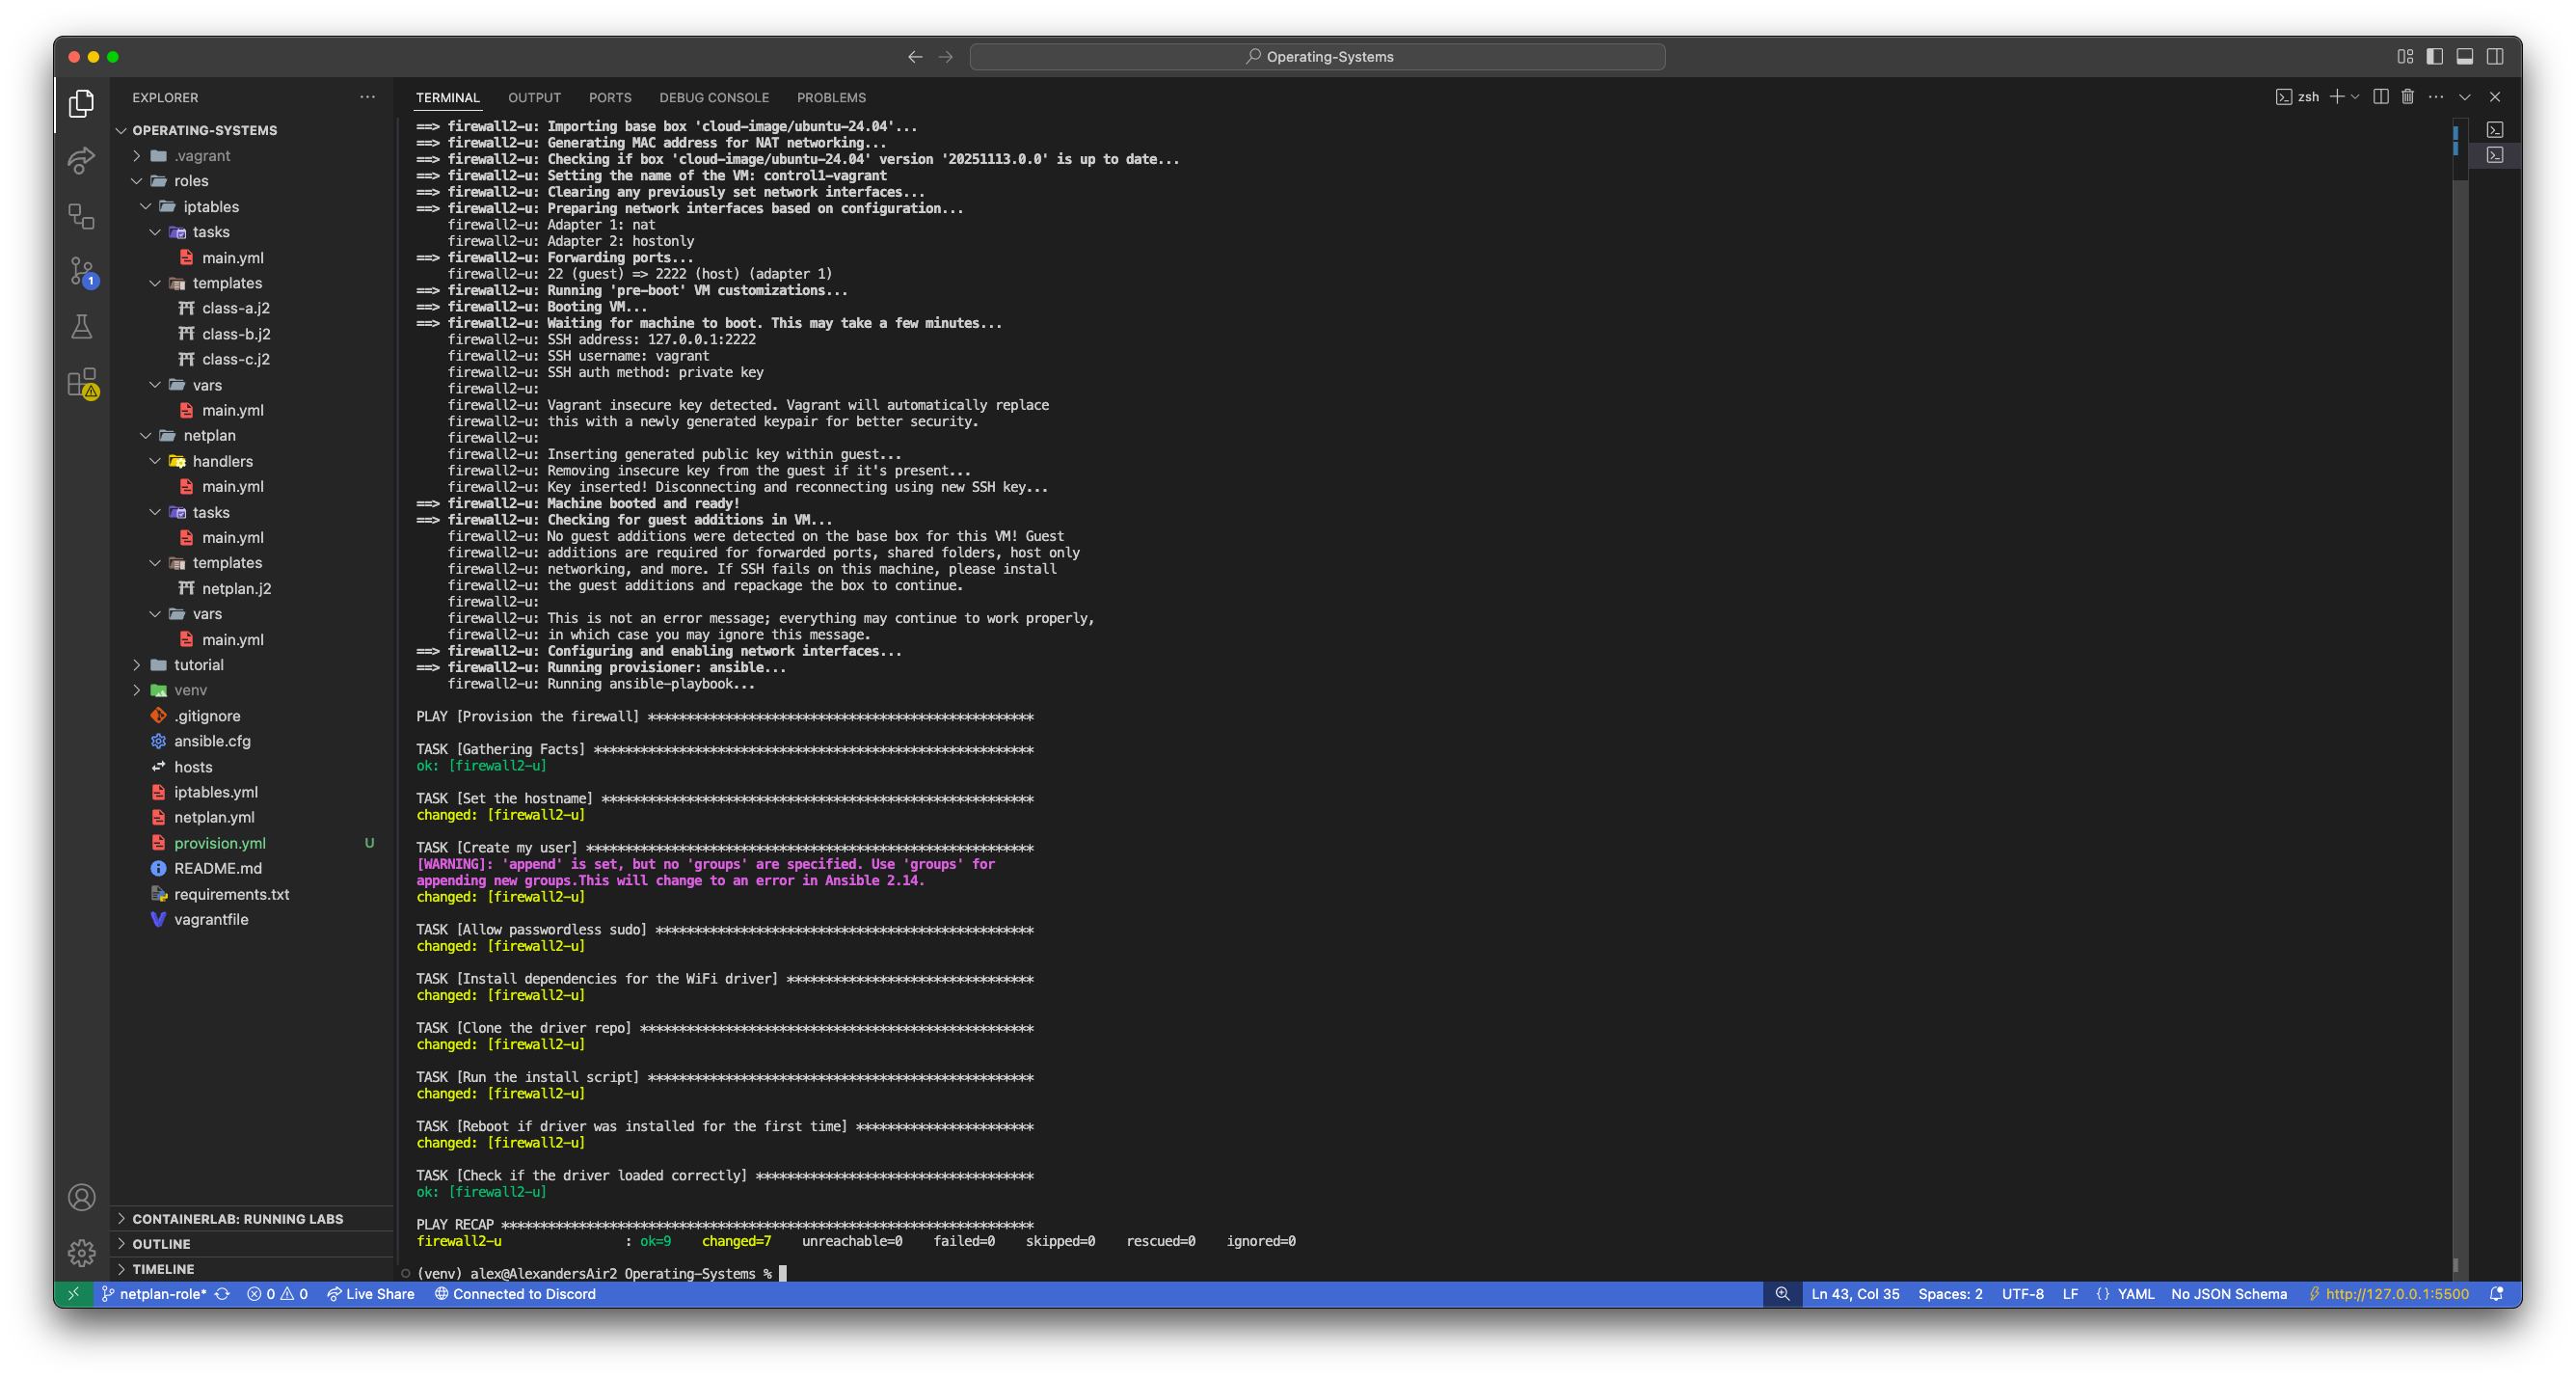
\includegraphics[width=\linewidth]{Screenshots/vscode-vagrant-provision.png}
    \caption{The output from bringing the provisioned VM with the driver up}
    \label{vagrant:provision-vm-nic}
\end{figure}

As the install was successful on the VM, it can be run on the production environment (Pi) and validated with \verb|| (figure \ref{vagrant:provision-firewall-nic}).

\begin{figure}[H]
    \centering
    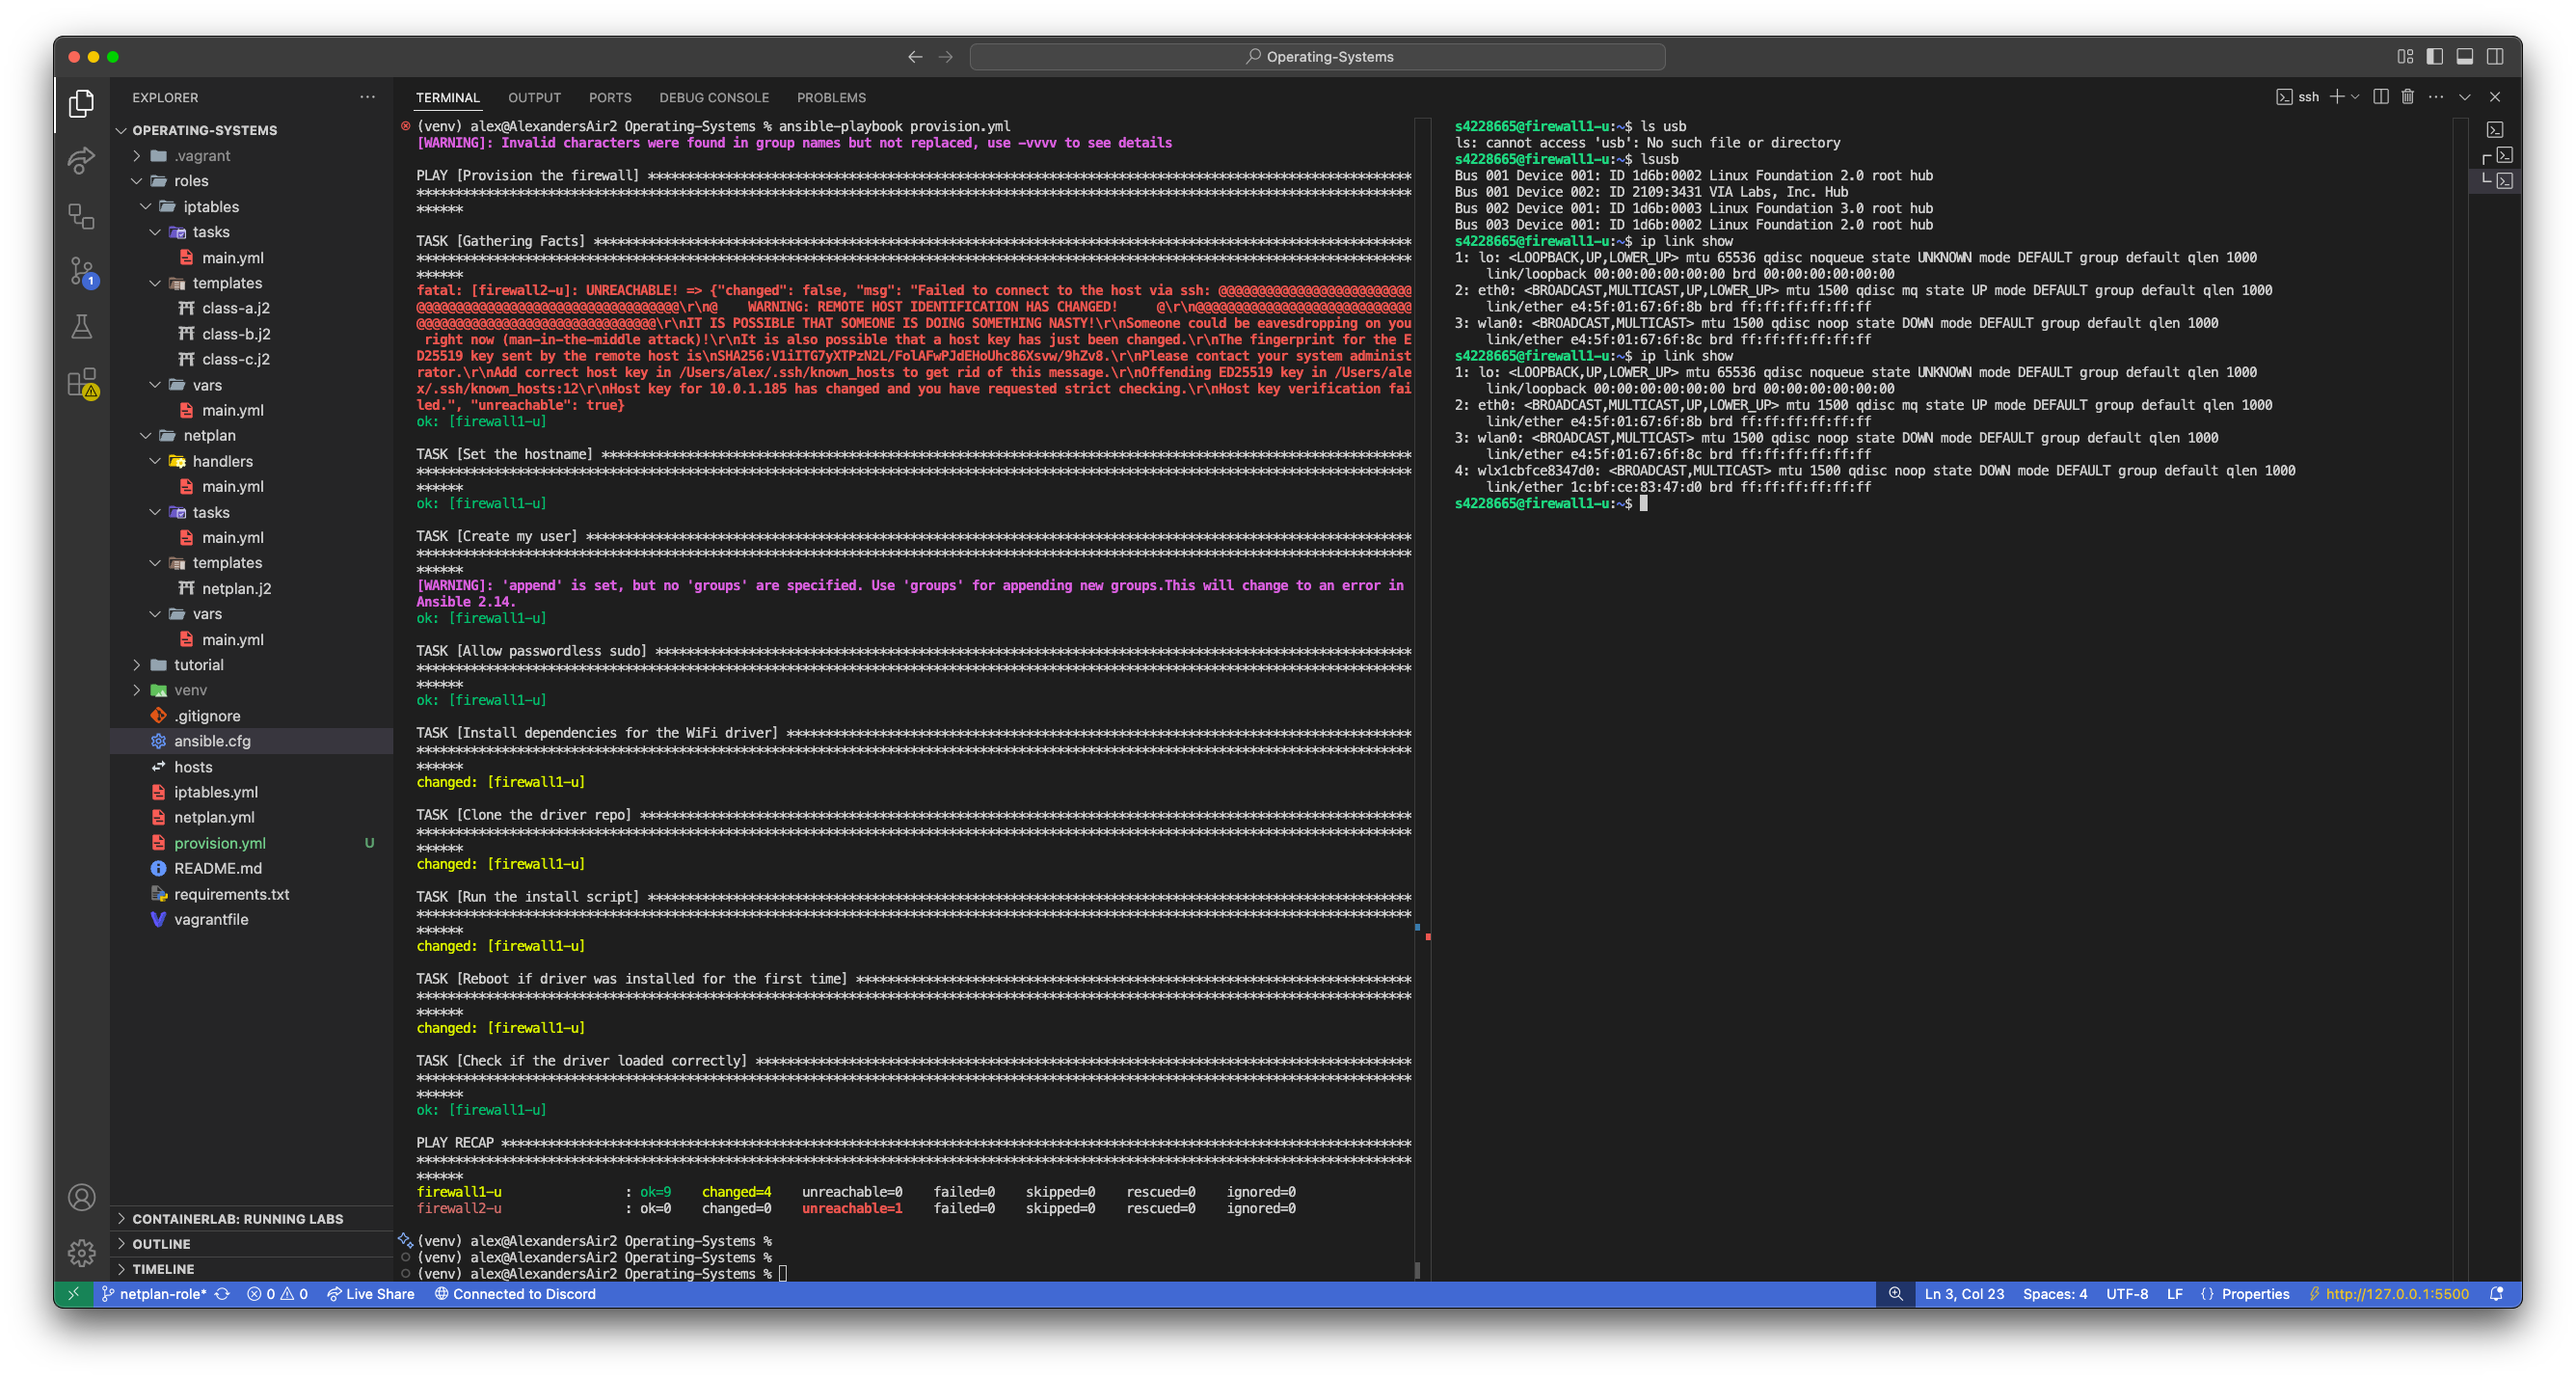
\includegraphics[width=\linewidth]{Screenshots/vscode-firewall-provision-validation.png}
    \caption{The output from bringing the provisioned VM with the driver up and it showing on the firewall}
    \label{vagrant:provision-firewall-nic}
\end{figure}

The output from \ref{vagrant:provision-vm-nic} shows the NIC is finally showing after unplugging and plugging the dongle back in after running the playbook. The interface came up as \verb|wlx1cbfce8347d0|. In adding to the playbook I had to go back and re-write it several times, namely because the driver interacts with the kernel so it needs to be compiled with Ubuntu's Dynamic Kernel Module Support (DKMS) package \parencite{Ubuntu2024DKMSDocumentation} so I needed to add the driver provided (by the VLE \parencite{Morrownr2024_8812au_Driver} but that didn't work). After installing it as intended nothing came up. 

I googled the output from \verb|lsusb| (figure \ref{fig:command-lsusb}) with drivers and the repo maintainer for both VLE suggested drivers as "Realtek c811 linux driver morrownr" and found a different (also unsupported) set of drivers \parencite{Morrownr2024_88x2bu_Driver} that worked.

\subsubsection{Multi-Interface Netplan Template}
\label{subsubsec:netplan-template}

The netplan configuration template (Figure \ref{code:ansible-netplan-template}) defines all three network interfaces with static IP addressing, DNS configuration, and routing rules.

\begin{figure}[H]
    \centering
    \begin{minted}{YAML}
    Nah, I'd win
    \end{minted}
    \caption{The jinja2 template used for configuring the interfaces}
    \label{code:ansible-netplan-template}
\end{figure}

In testing this on the VM firewall (with variables from figure \ref{fig:netplan-vars} and deploying in figure \ref{vagrant:netplan-deploy}), I noticed this won't work as well as the real firewall as the hardware setup isn't the same. While having a virtual machine (an easily destructible testing environment) is good for validating config changes, there are limitations.

\begin{figure}[H]
    \centering
    \begin{minted}{YAML}
    Nah, I'd win
    \end{minted}
    \caption{The Jinja2 template used for configuring the interfaces}
    \label{code:ansible-netplan-vars}
\end{figure}

\begin{figure}[H]
    \centering
    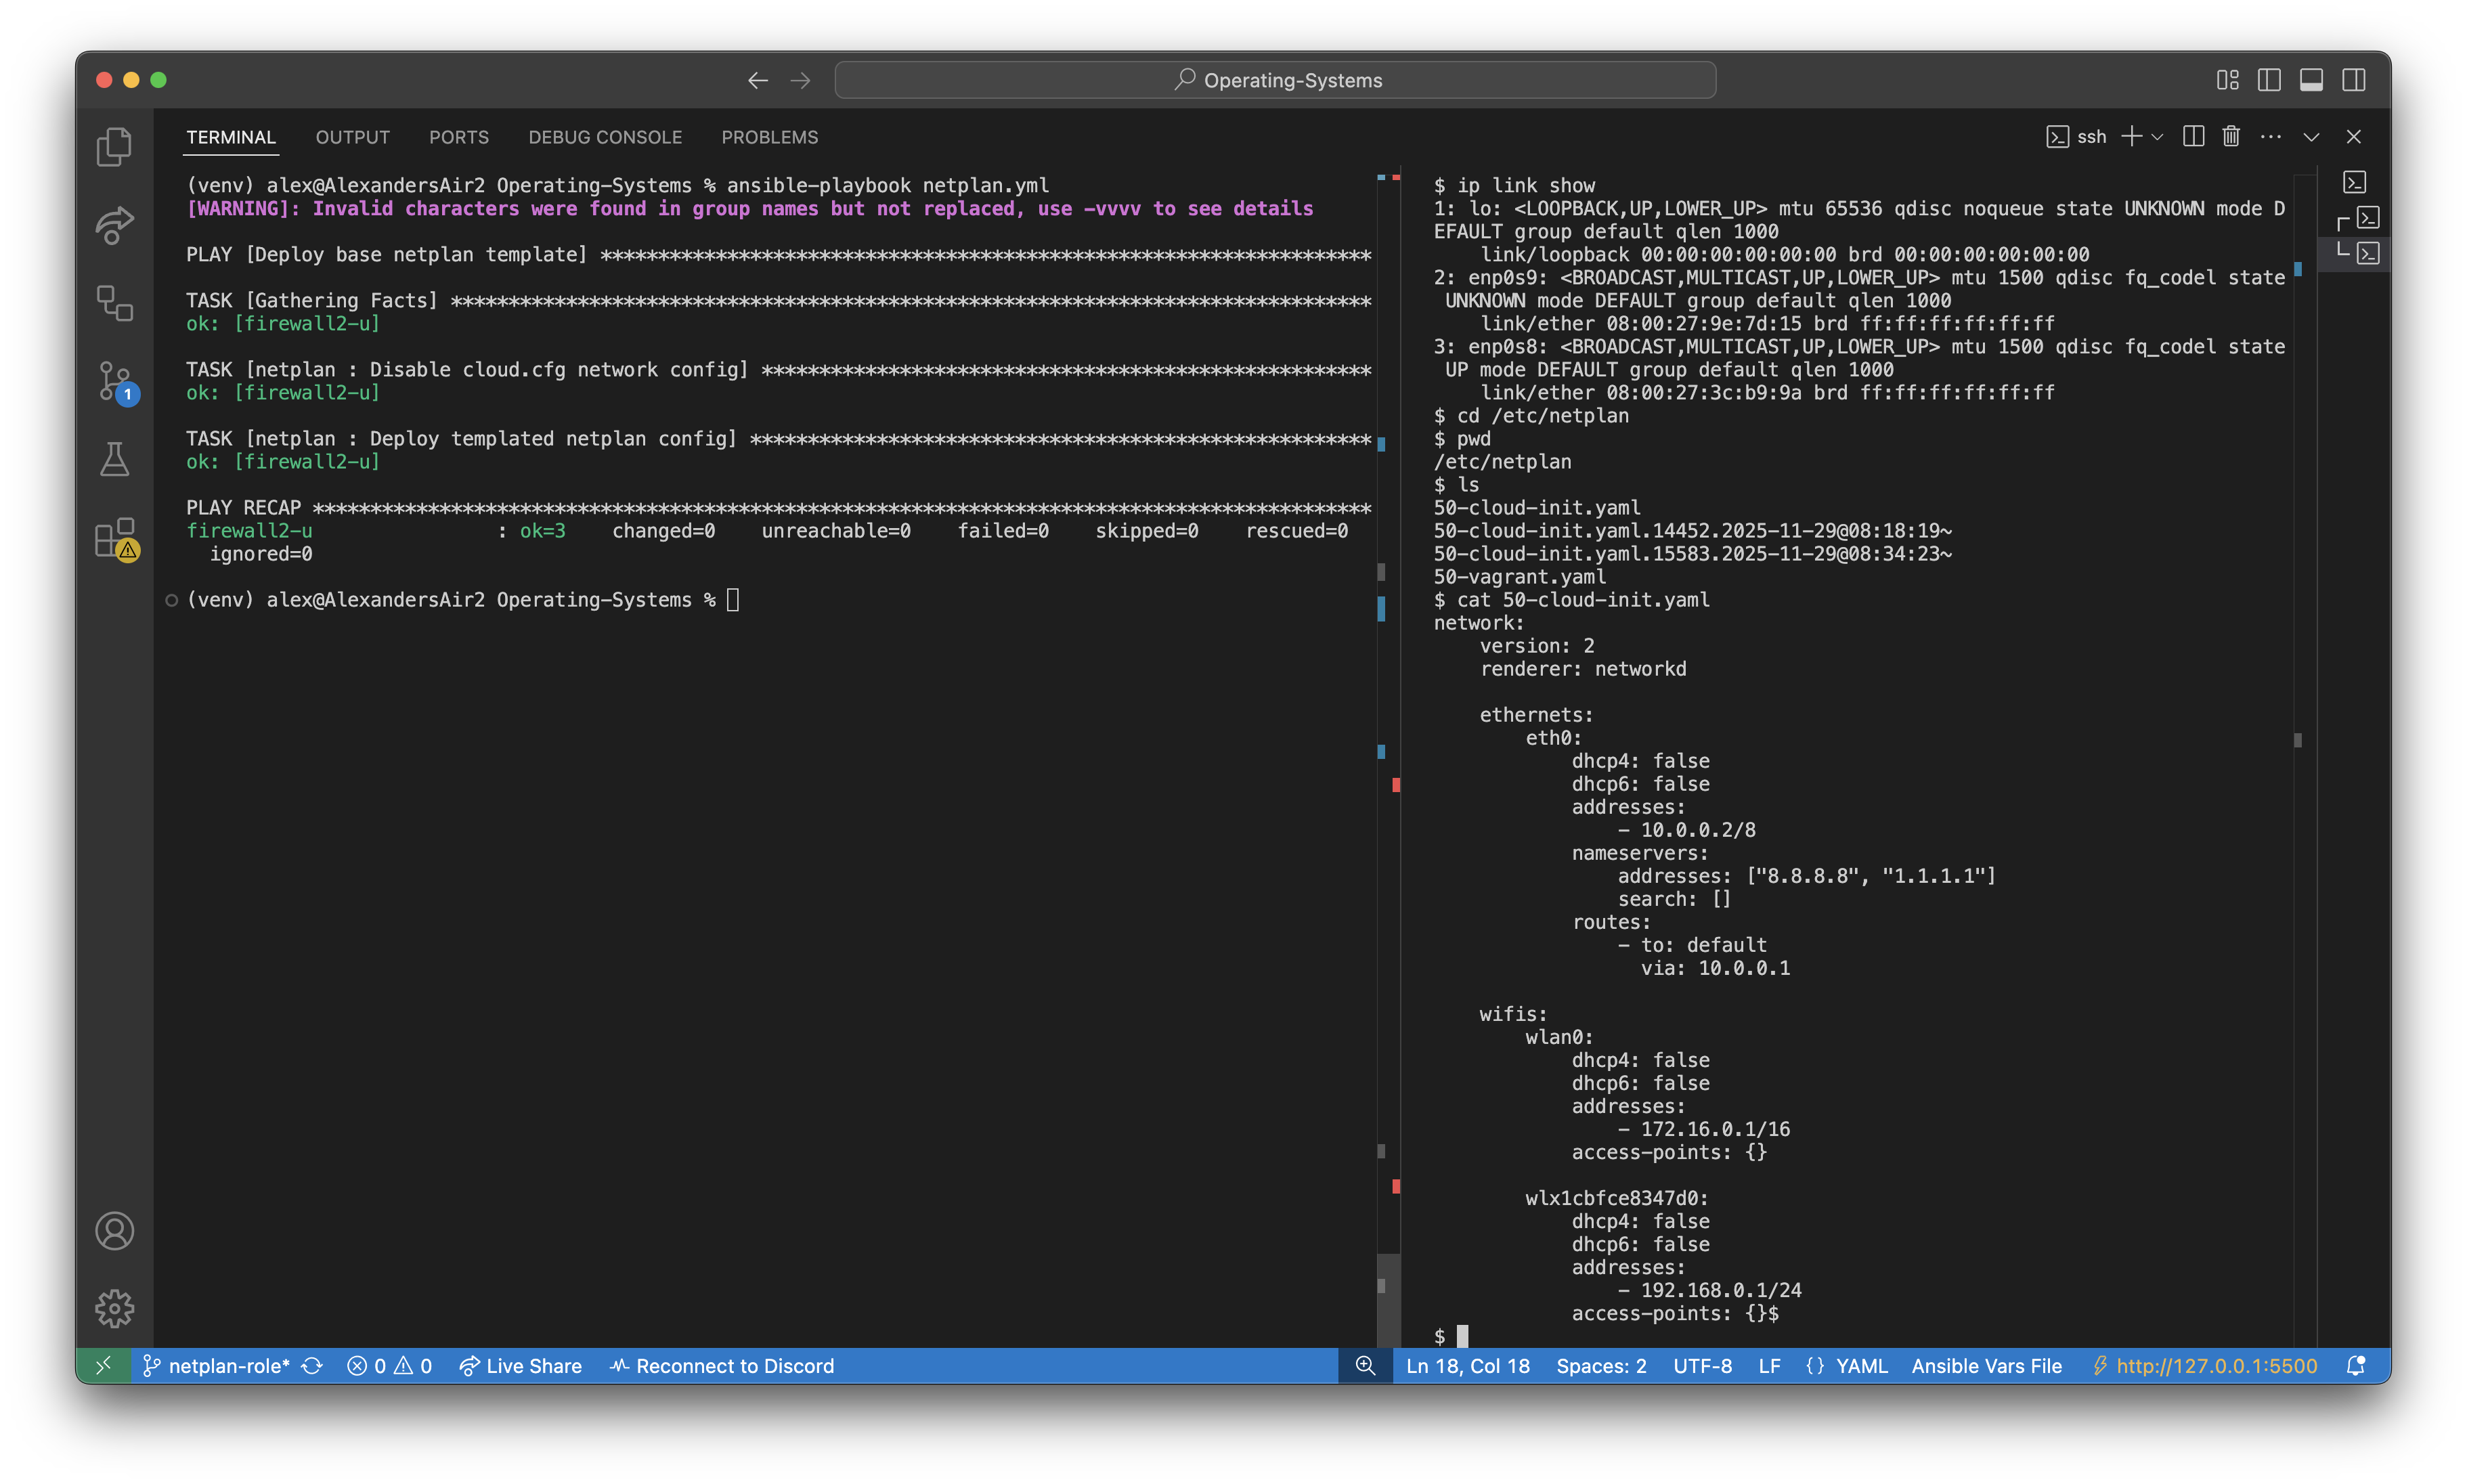
\includegraphics[width=1\linewidth]{Screenshots/vscode-vagrant-netplan-deploy.png}
    \caption{Side by side viewing of the successful netplan deploy (left) and the applied netplan config (right)}
    \label{vagrant:netplan-deploy}
\end{figure}

As the deploy was validated on the VM, the config can be deployed to the firewall.

\begin{figure}[H]
    \centering
    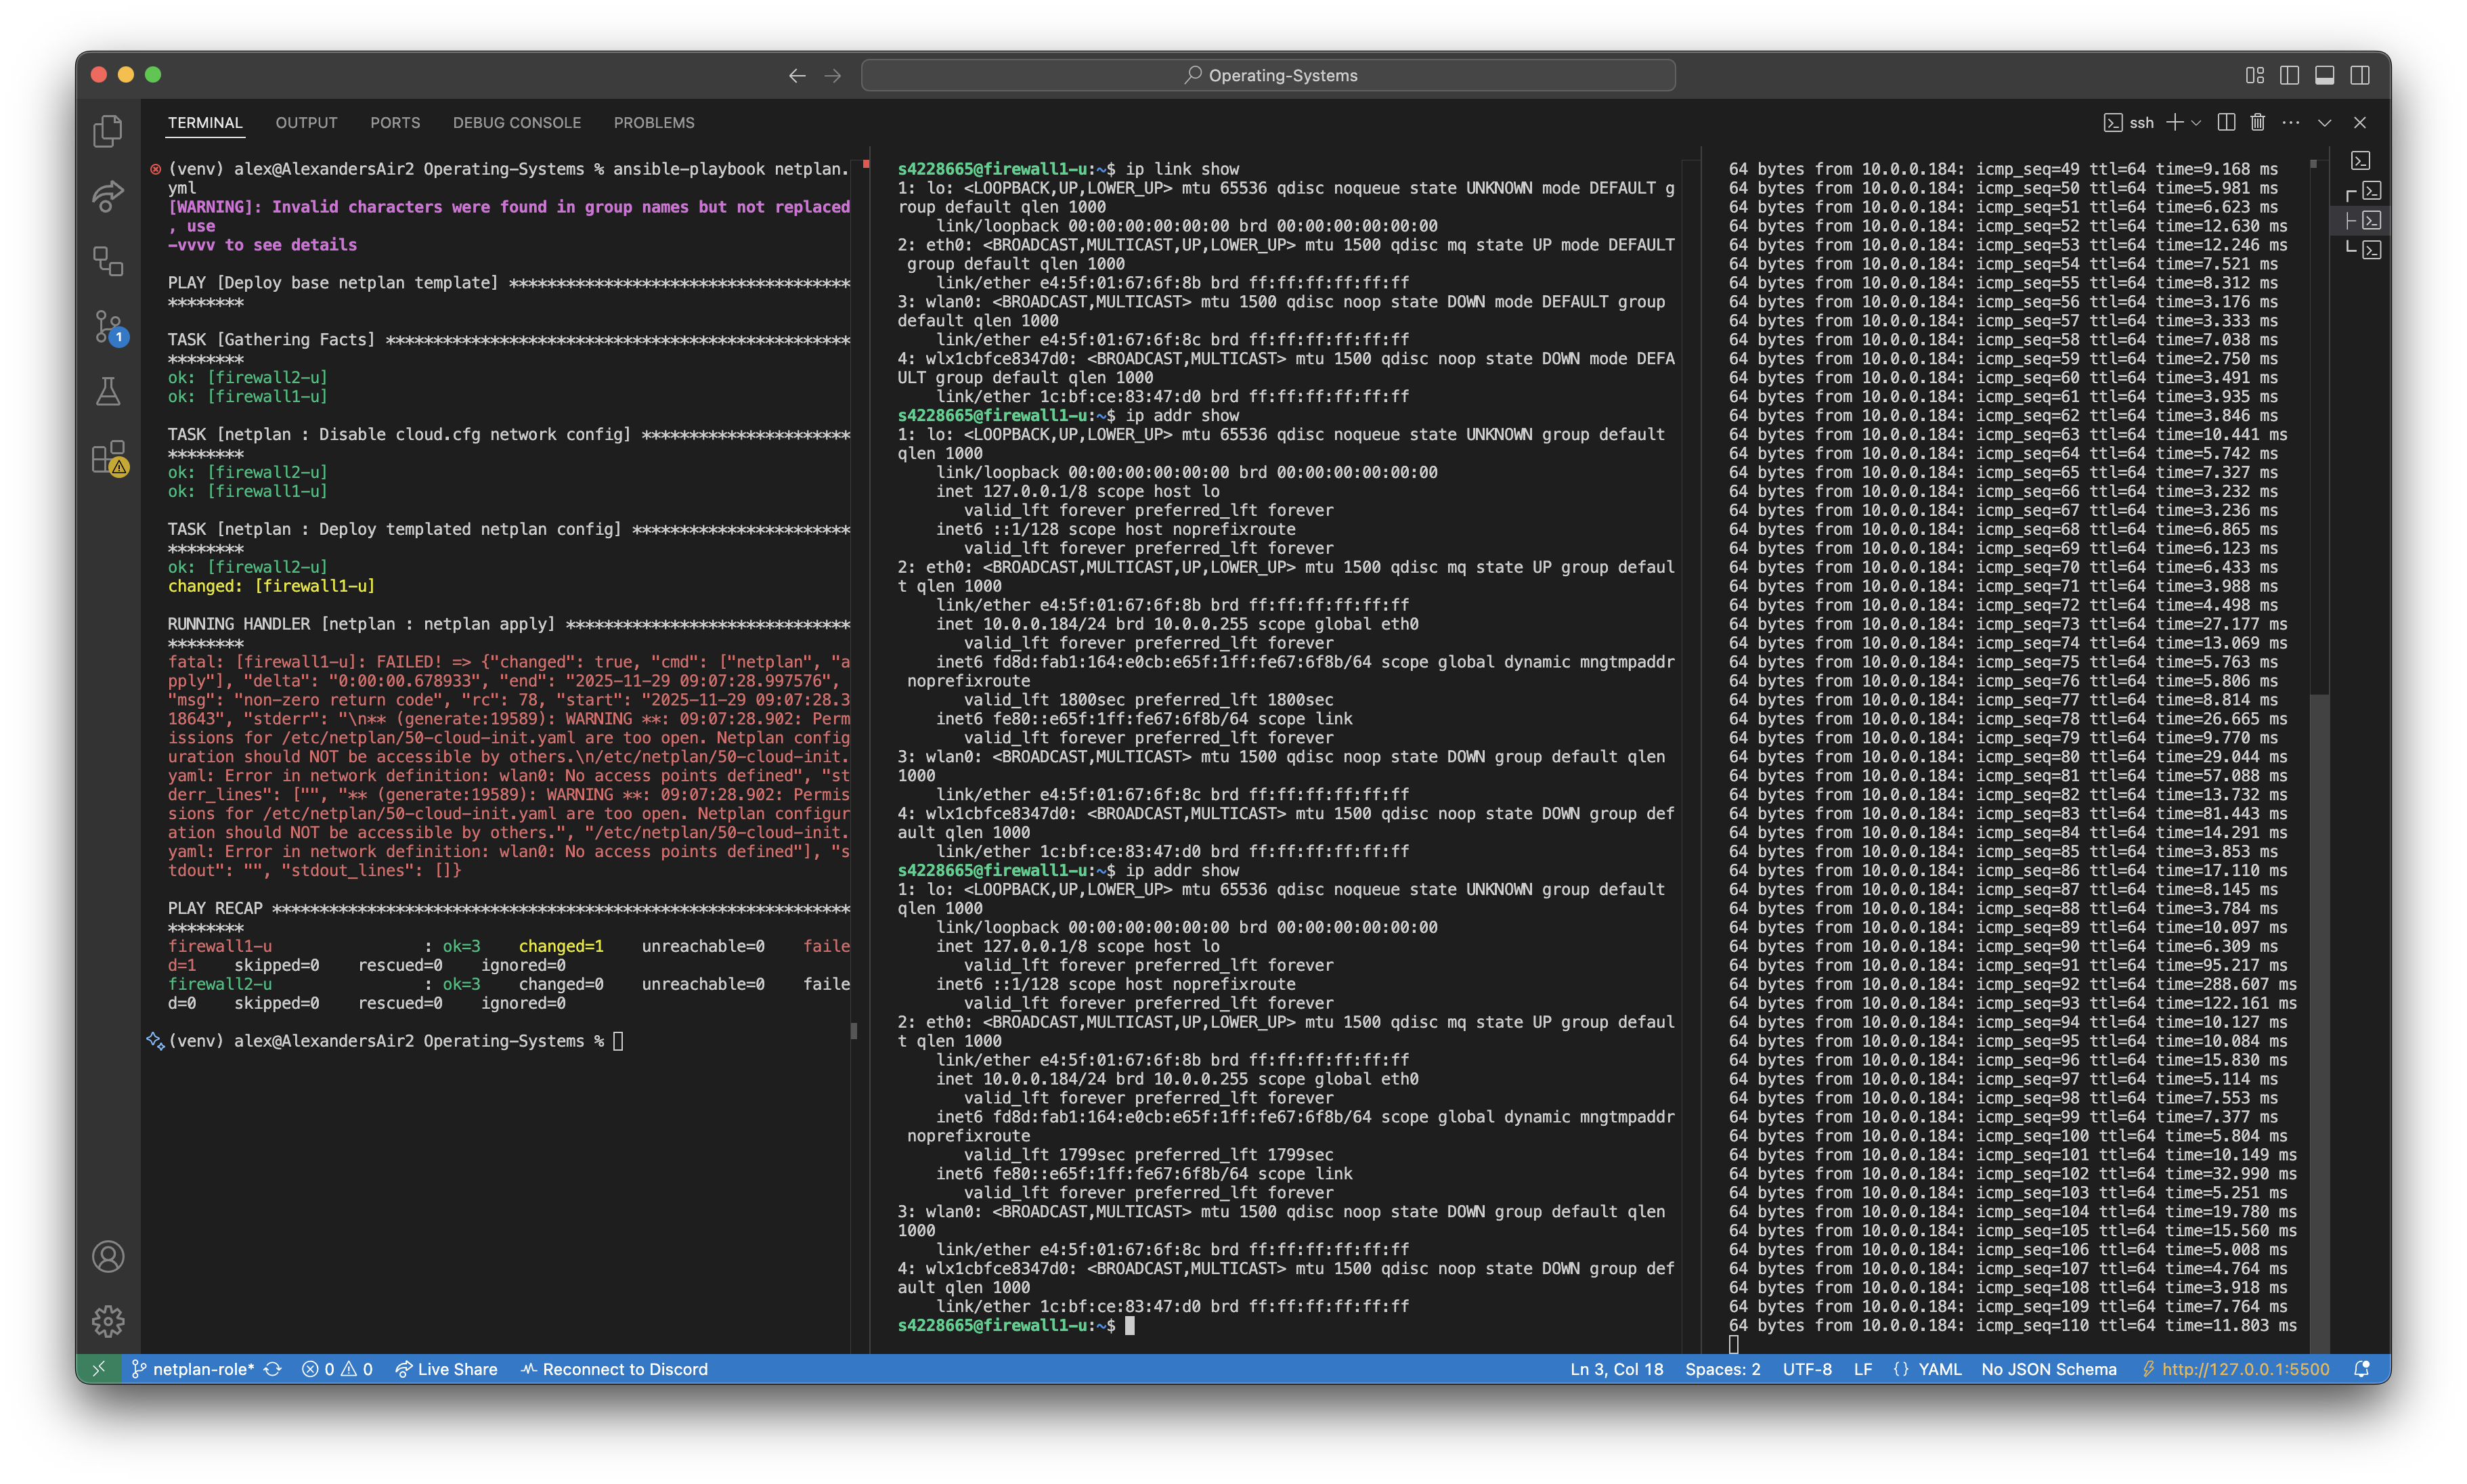
\includegraphics[width=1\linewidth]{Screenshots/vscode-both-neplan-deploy.png}
    \caption{View of the deploy to both firewalls (left), a SSH session to the firewall showing the before and after states of the netplan deploy (centre) and a running ping to confirm if something went wrong while deploying the config (right)}
    \label{fig:combined-netplan-deploy}
\end{figure}

The centre part of figure \ref{fig:combined-netplan-deploy} shows the two NICs as down, after trying to bring them up manually I realised they need to be configured as access-points, not as WiFi clients. Netplan doesn't support this but hostapd \parencite{LinuxKernel2024HostapdDocumentation} \parencite{Hostapd2024Documentation} does.

On Linux operating systems, WiFi interfaces being used as access points (APs) need the hostapd daemon to manage client authentication, and beacon broadcasting \parencite{Hostapd2024Documentation}. Netplan configures IP addressing and routing at the network layer (Layer 3), but hostapd operates at the data link and physical layers (Layers 1 and 2) to establish the wireless medium.

To use hostapd (with logging), you need to use systemd services \parencite{Freedesktop2024Systemd} to give a level of persistence via \texttt{WantedBy=multi-user.target}. A systemd service will enable the hostapd daemons to start after network initialisation (\texttt{After=network.target}) and automatically restart on failure (\texttt{Restart=on-failure}). This isn't needed for netplan or iptables as netplan is persistant and iptables uses an additional module (REFERNECE TO IPTABLESROLE PERSISTANCE) to keep the config active.

As hostapd can be defined as systemd services, it fits nicely into the Ansible IaC approach, as this can be sorted into a new role defined as figure \ref{fig:ansible-hostapd-role}.

\begin{figure}[H]
    \centering
    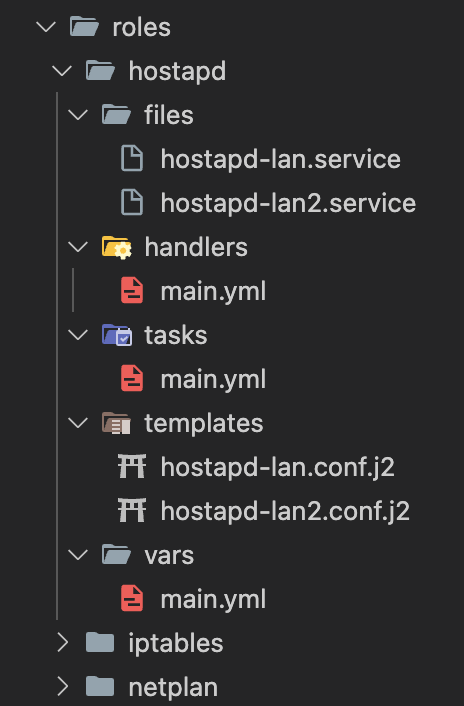
\includegraphics[width=0.5\linewidth]{Screenshots/vscode-hostapd-role.png}
    \caption{The new role structure for hostapd}
    \label{fig:ansible-hostapd-role}
\end{figure}

. This architecture follows established patterns for Raspberry Pi wireless access point deployment \parencite{RaspberryPi2024Documentation}, separating Layer 2 wireless management (hostapd) from Layer 3 network configuration (netplan) for modular, maintainable infrastructure automation.

\begin{figure}[H]
    \centering
    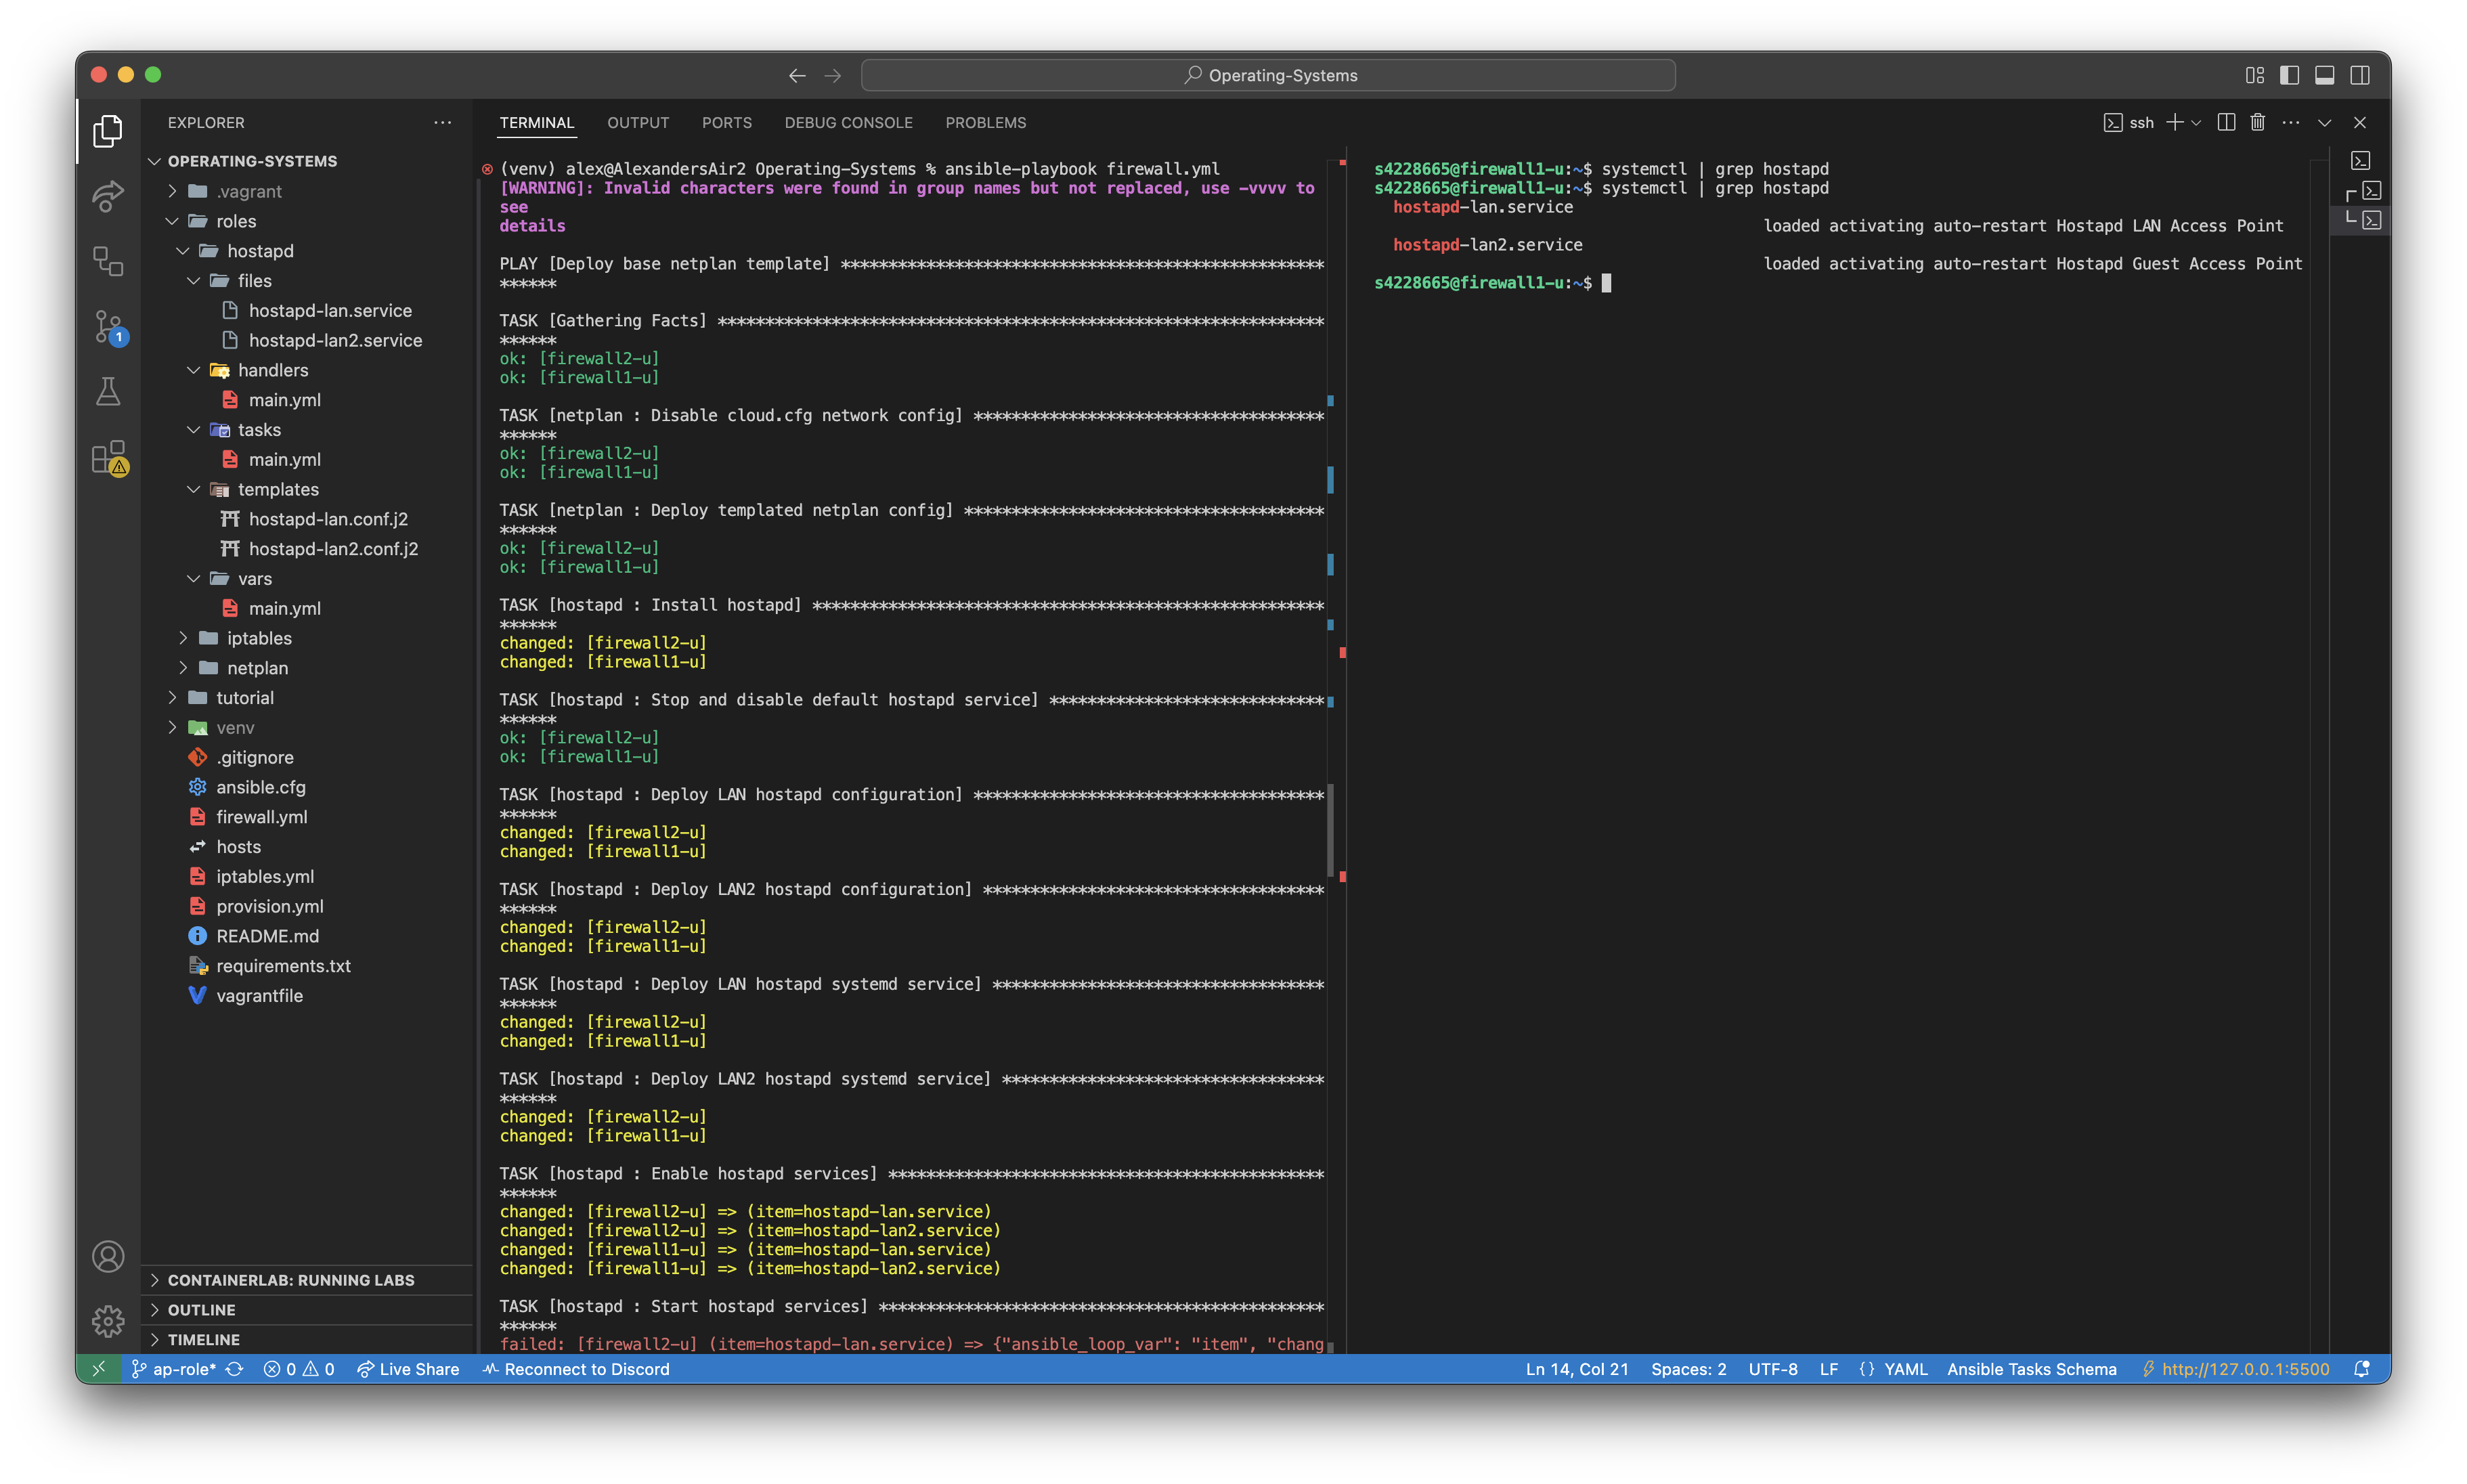
\includegraphics[width=1\linewidth]{Screenshots/vscode-both-hostapd-deploy.png}
    \caption{First deploy of the hostapd role (left) and the services running on the firewall (right)}
    \label{fig:ansible-hostapd-deploy}
\end{figure}


\begin{figure}[H]
    \centering
    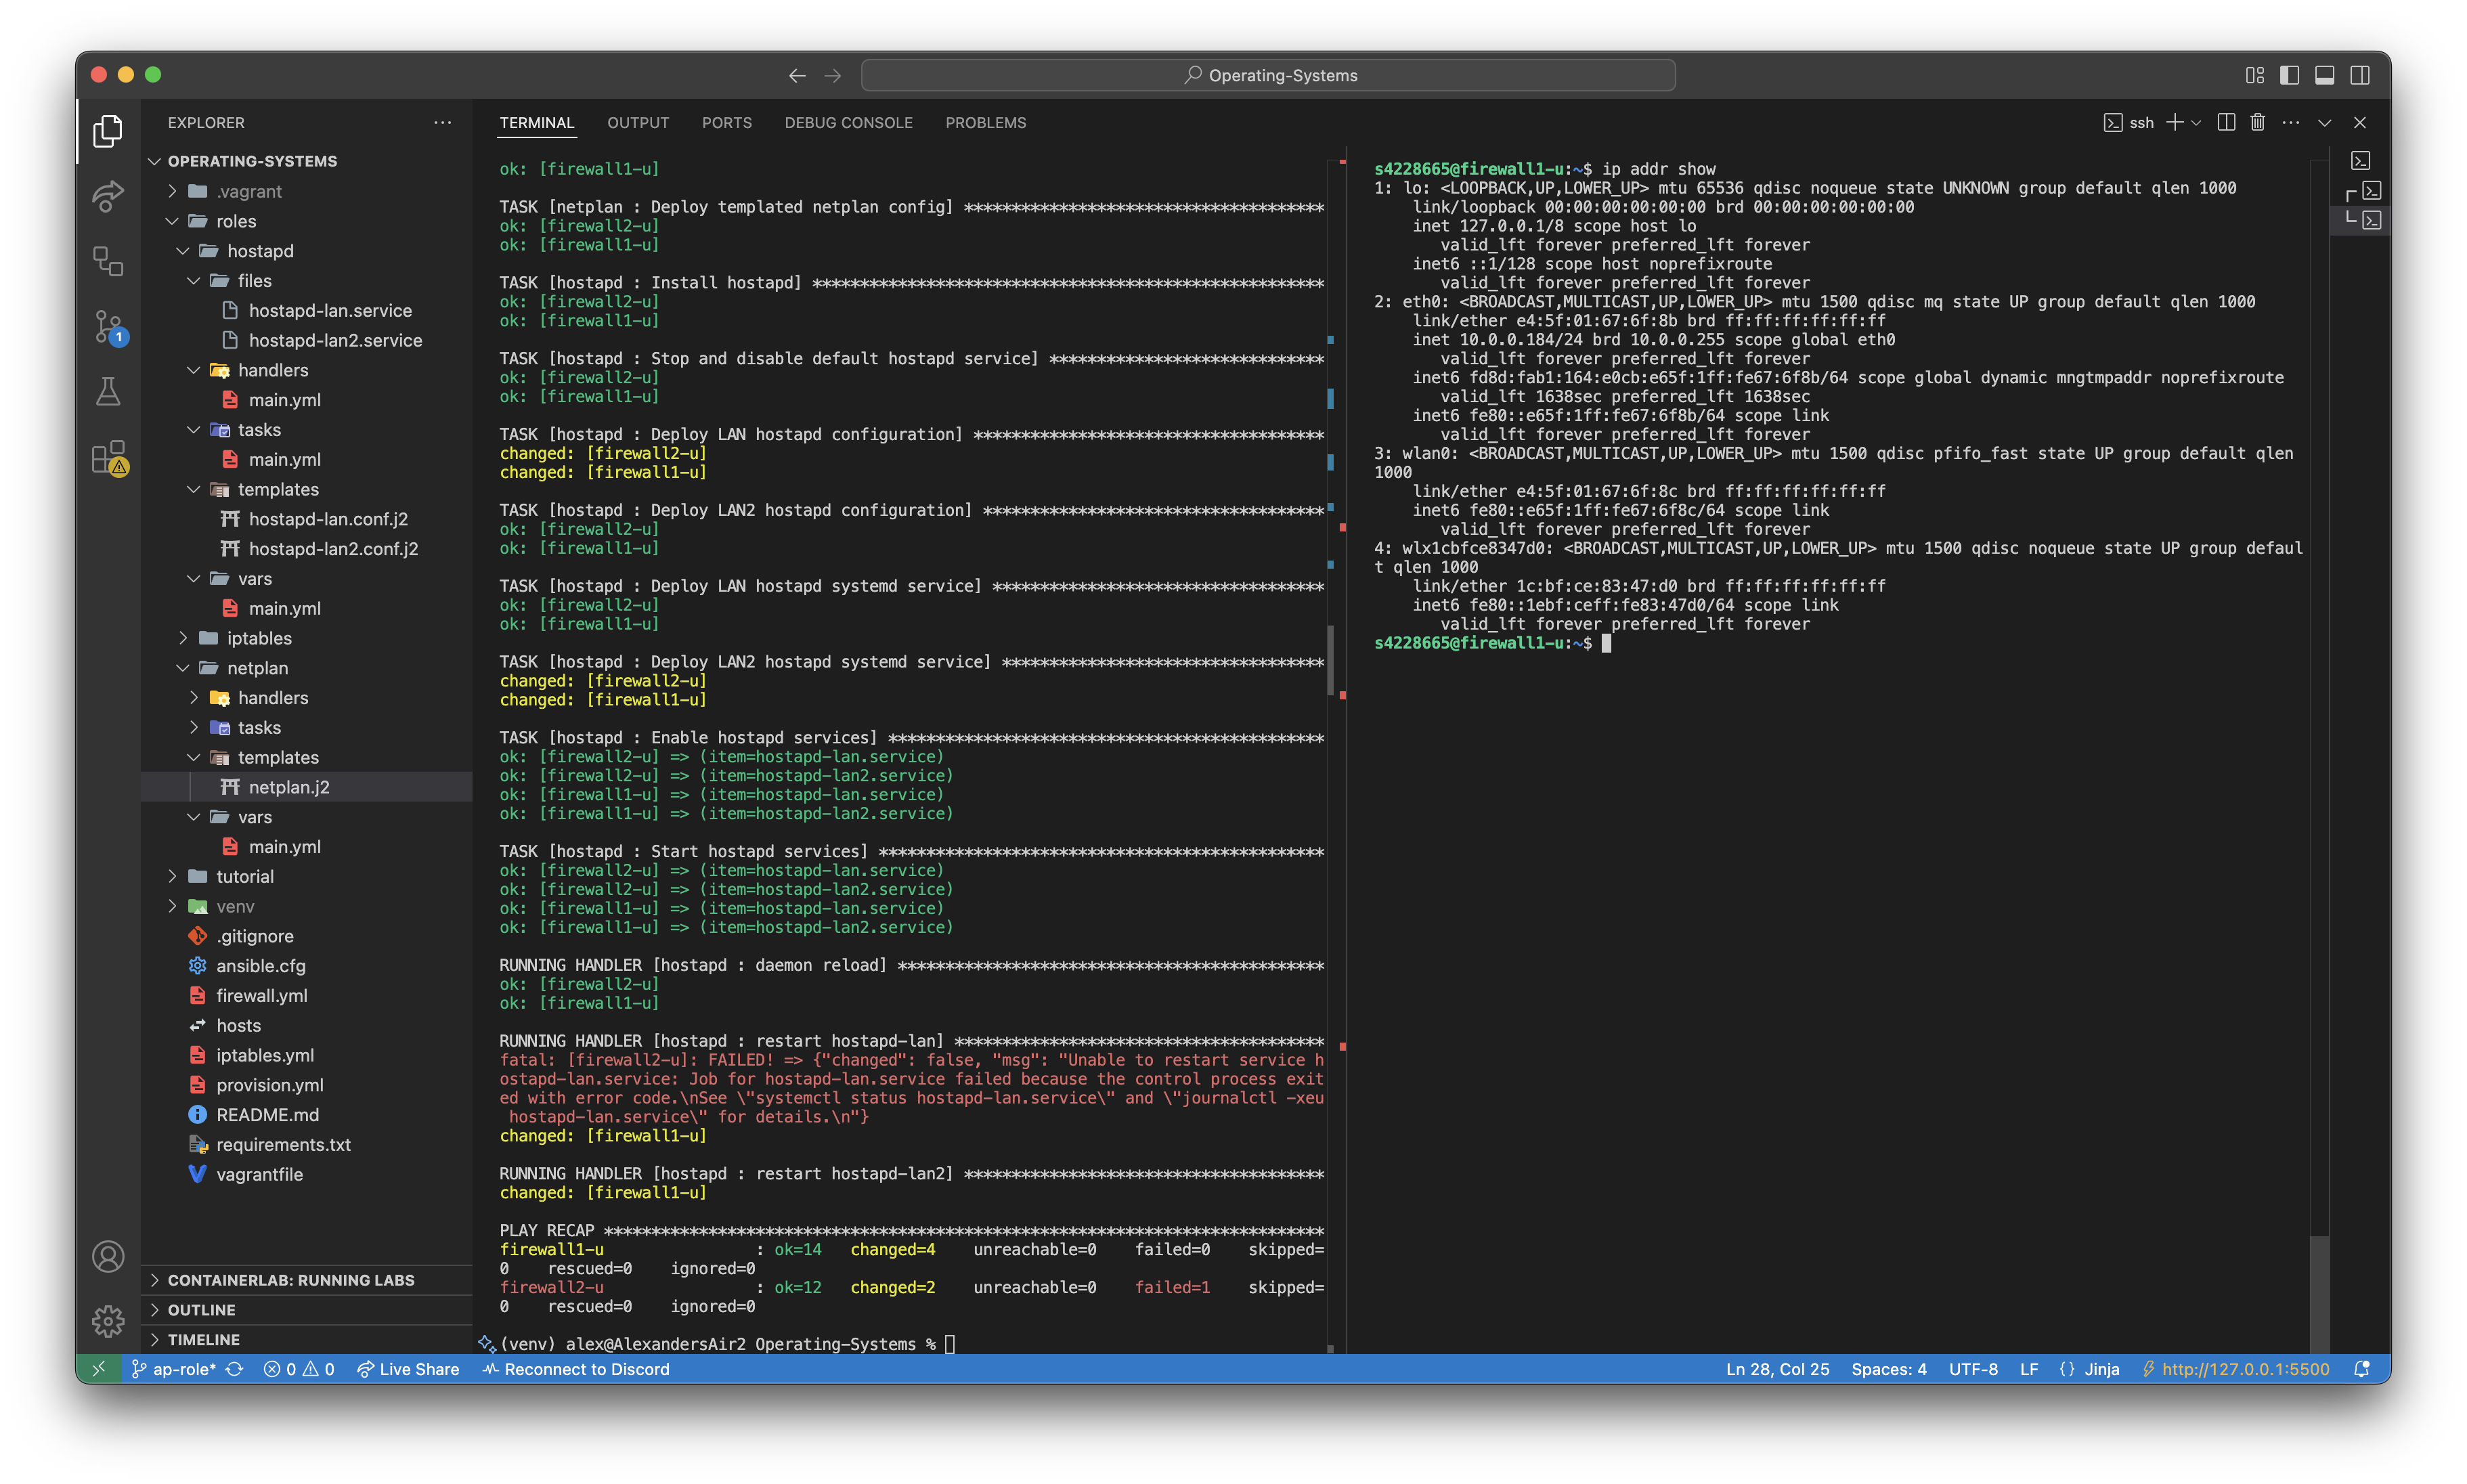
\includegraphics[width=1\linewidth]{Screenshots/vscode-both-hostapd-deploy2.png}
    \caption{Enter Caption}
    \label{fig:placeholder}
\end{figure}

Something something the 5G SSID was showing up but not the 2.4G one, and it could be related to one of the handlers failing on the main firewall - this is expected on the VM as it's not running on the hardware, at this point I decided to start changing the netplan + hostapd config, the extent of which can be seen in this pull request (REFERNECE PULL REQUEST WITH CHANGES). To validate the changes, I worked from my laptop and the VM firewall (figure \ref{fig:ansible-hostapd+netplan-deploy-test}).

\begin{figure}[H]
    \centering
    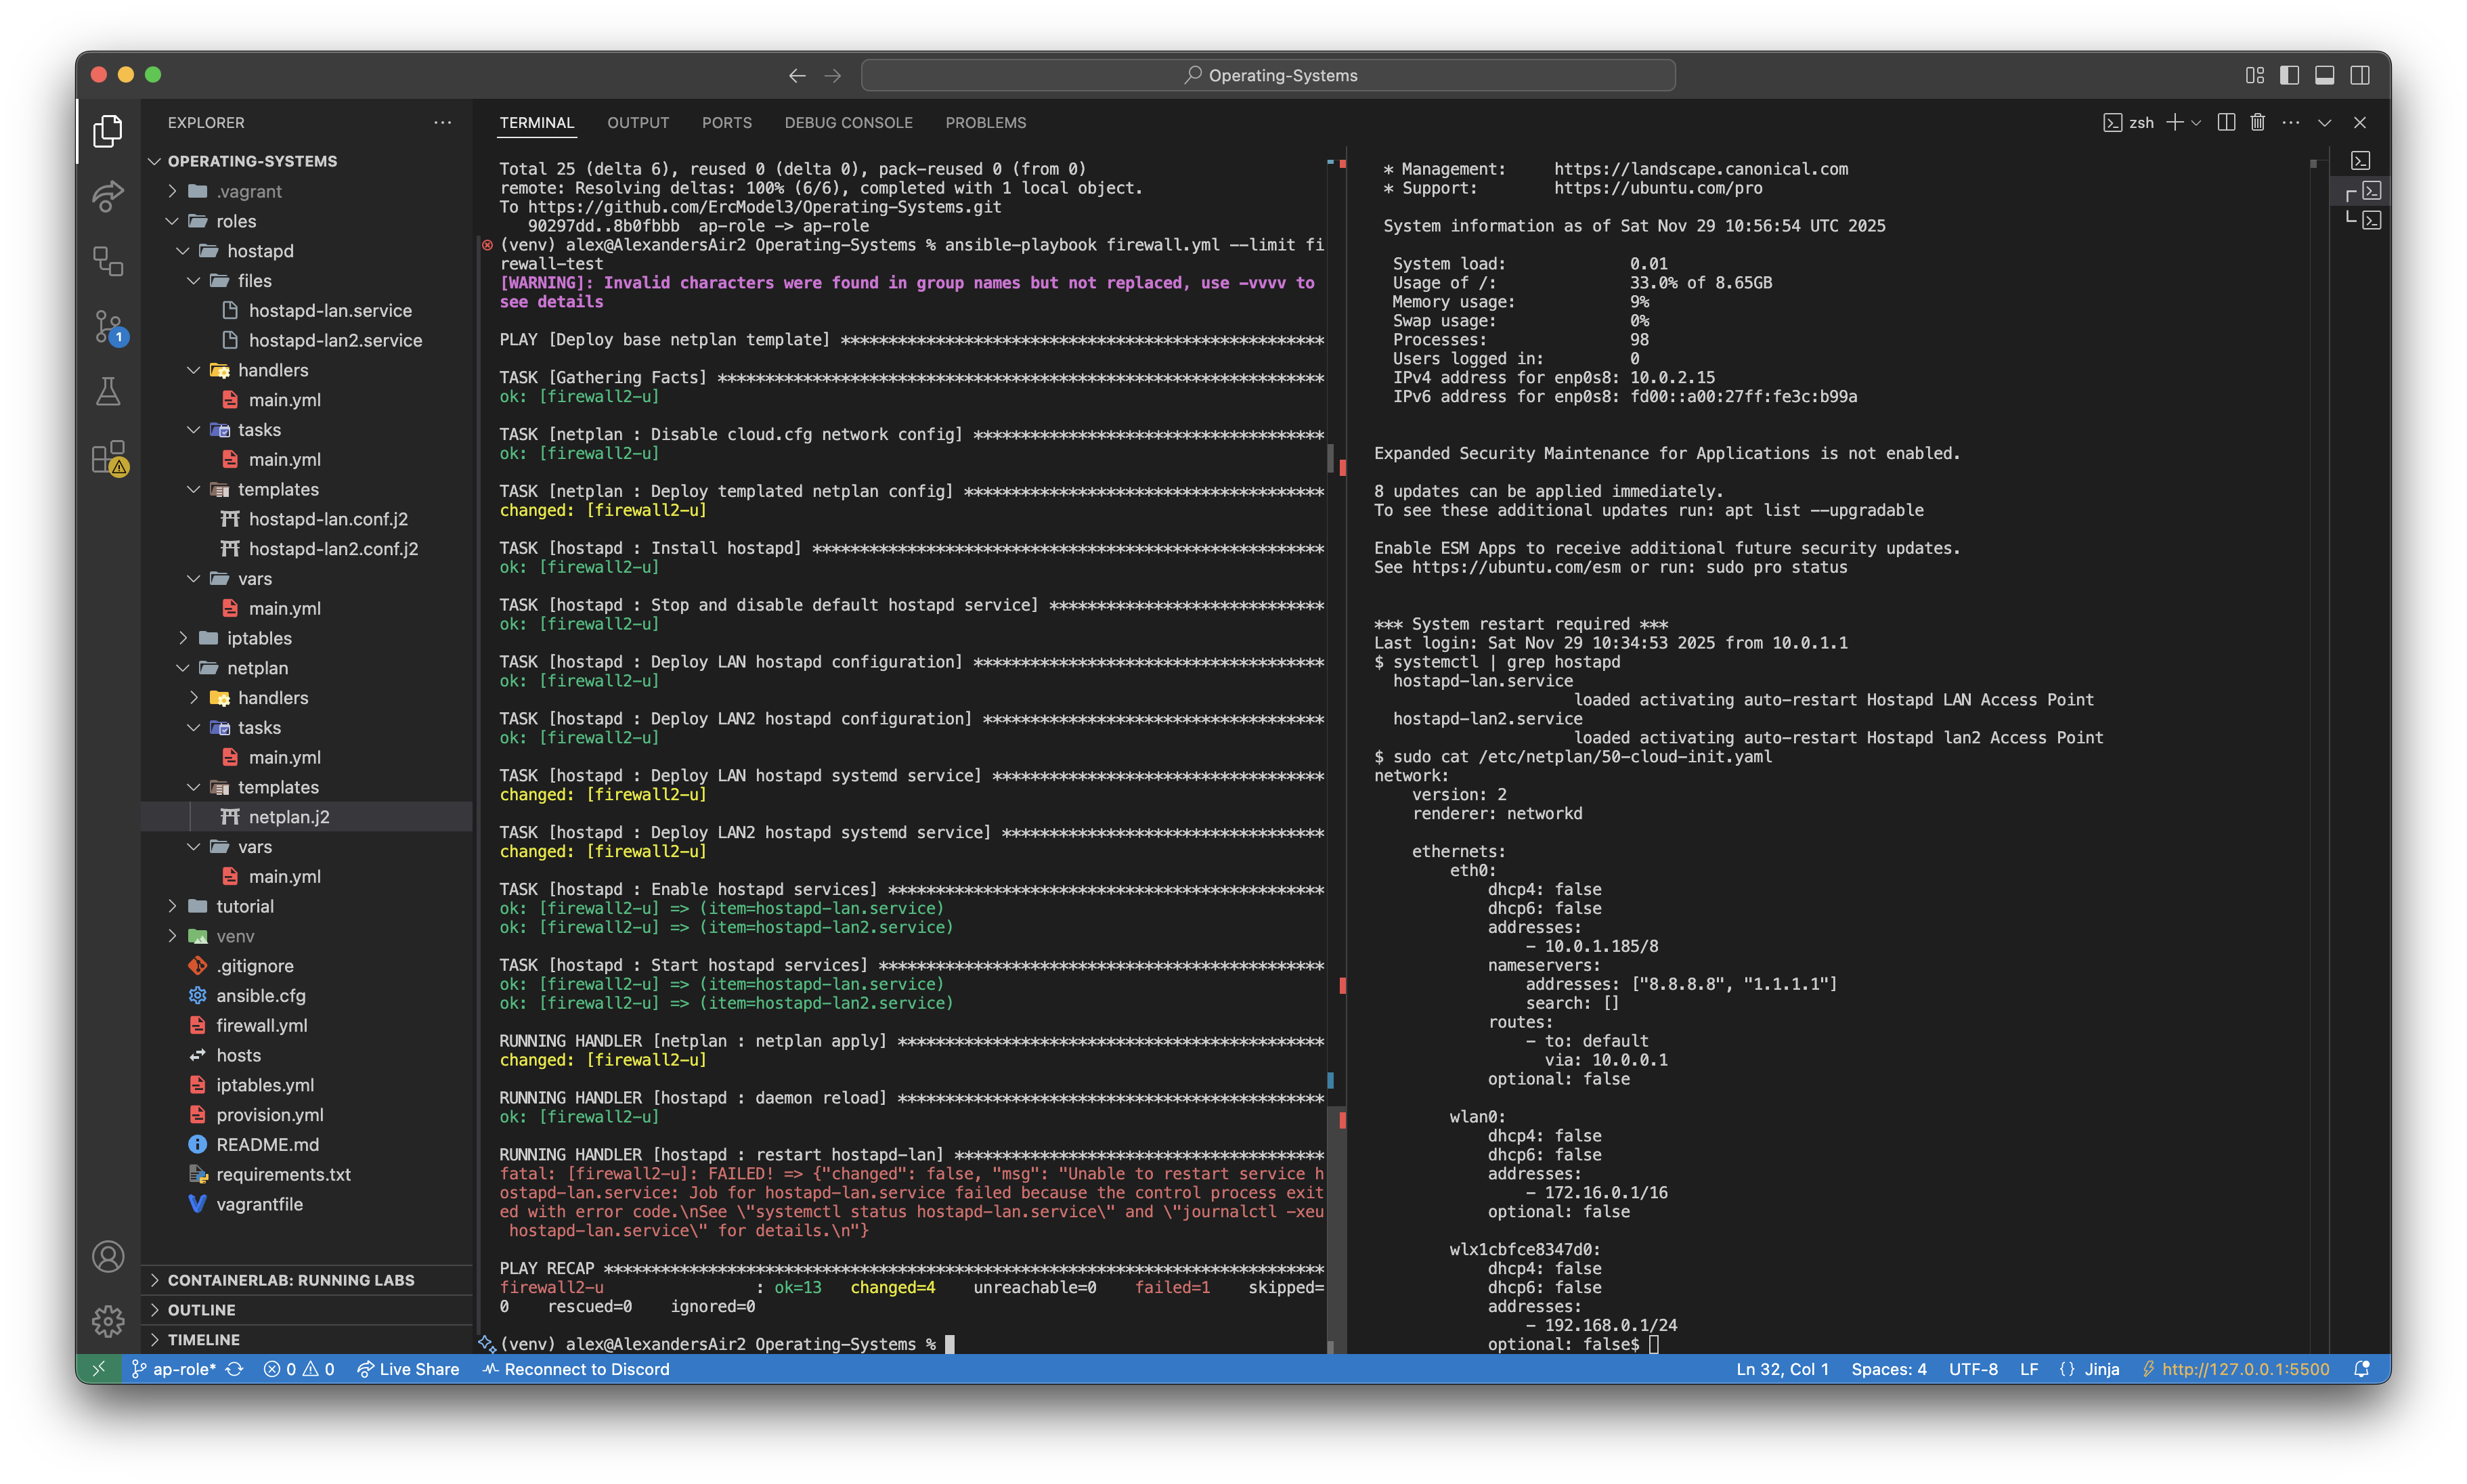
\includegraphics[width=1\linewidth]{Screenshots/image.png}
    \caption{Enter Caption}
    \label{fig:ansible-hostapd+netplan-deploy-test}
\end{figure}

And after a successful deploy, it was time to push it to the firewall (figure \ref{fig:ansible-hostapd+netplan-deploy-prod}).

\begin{figure}[H]
    \centering
    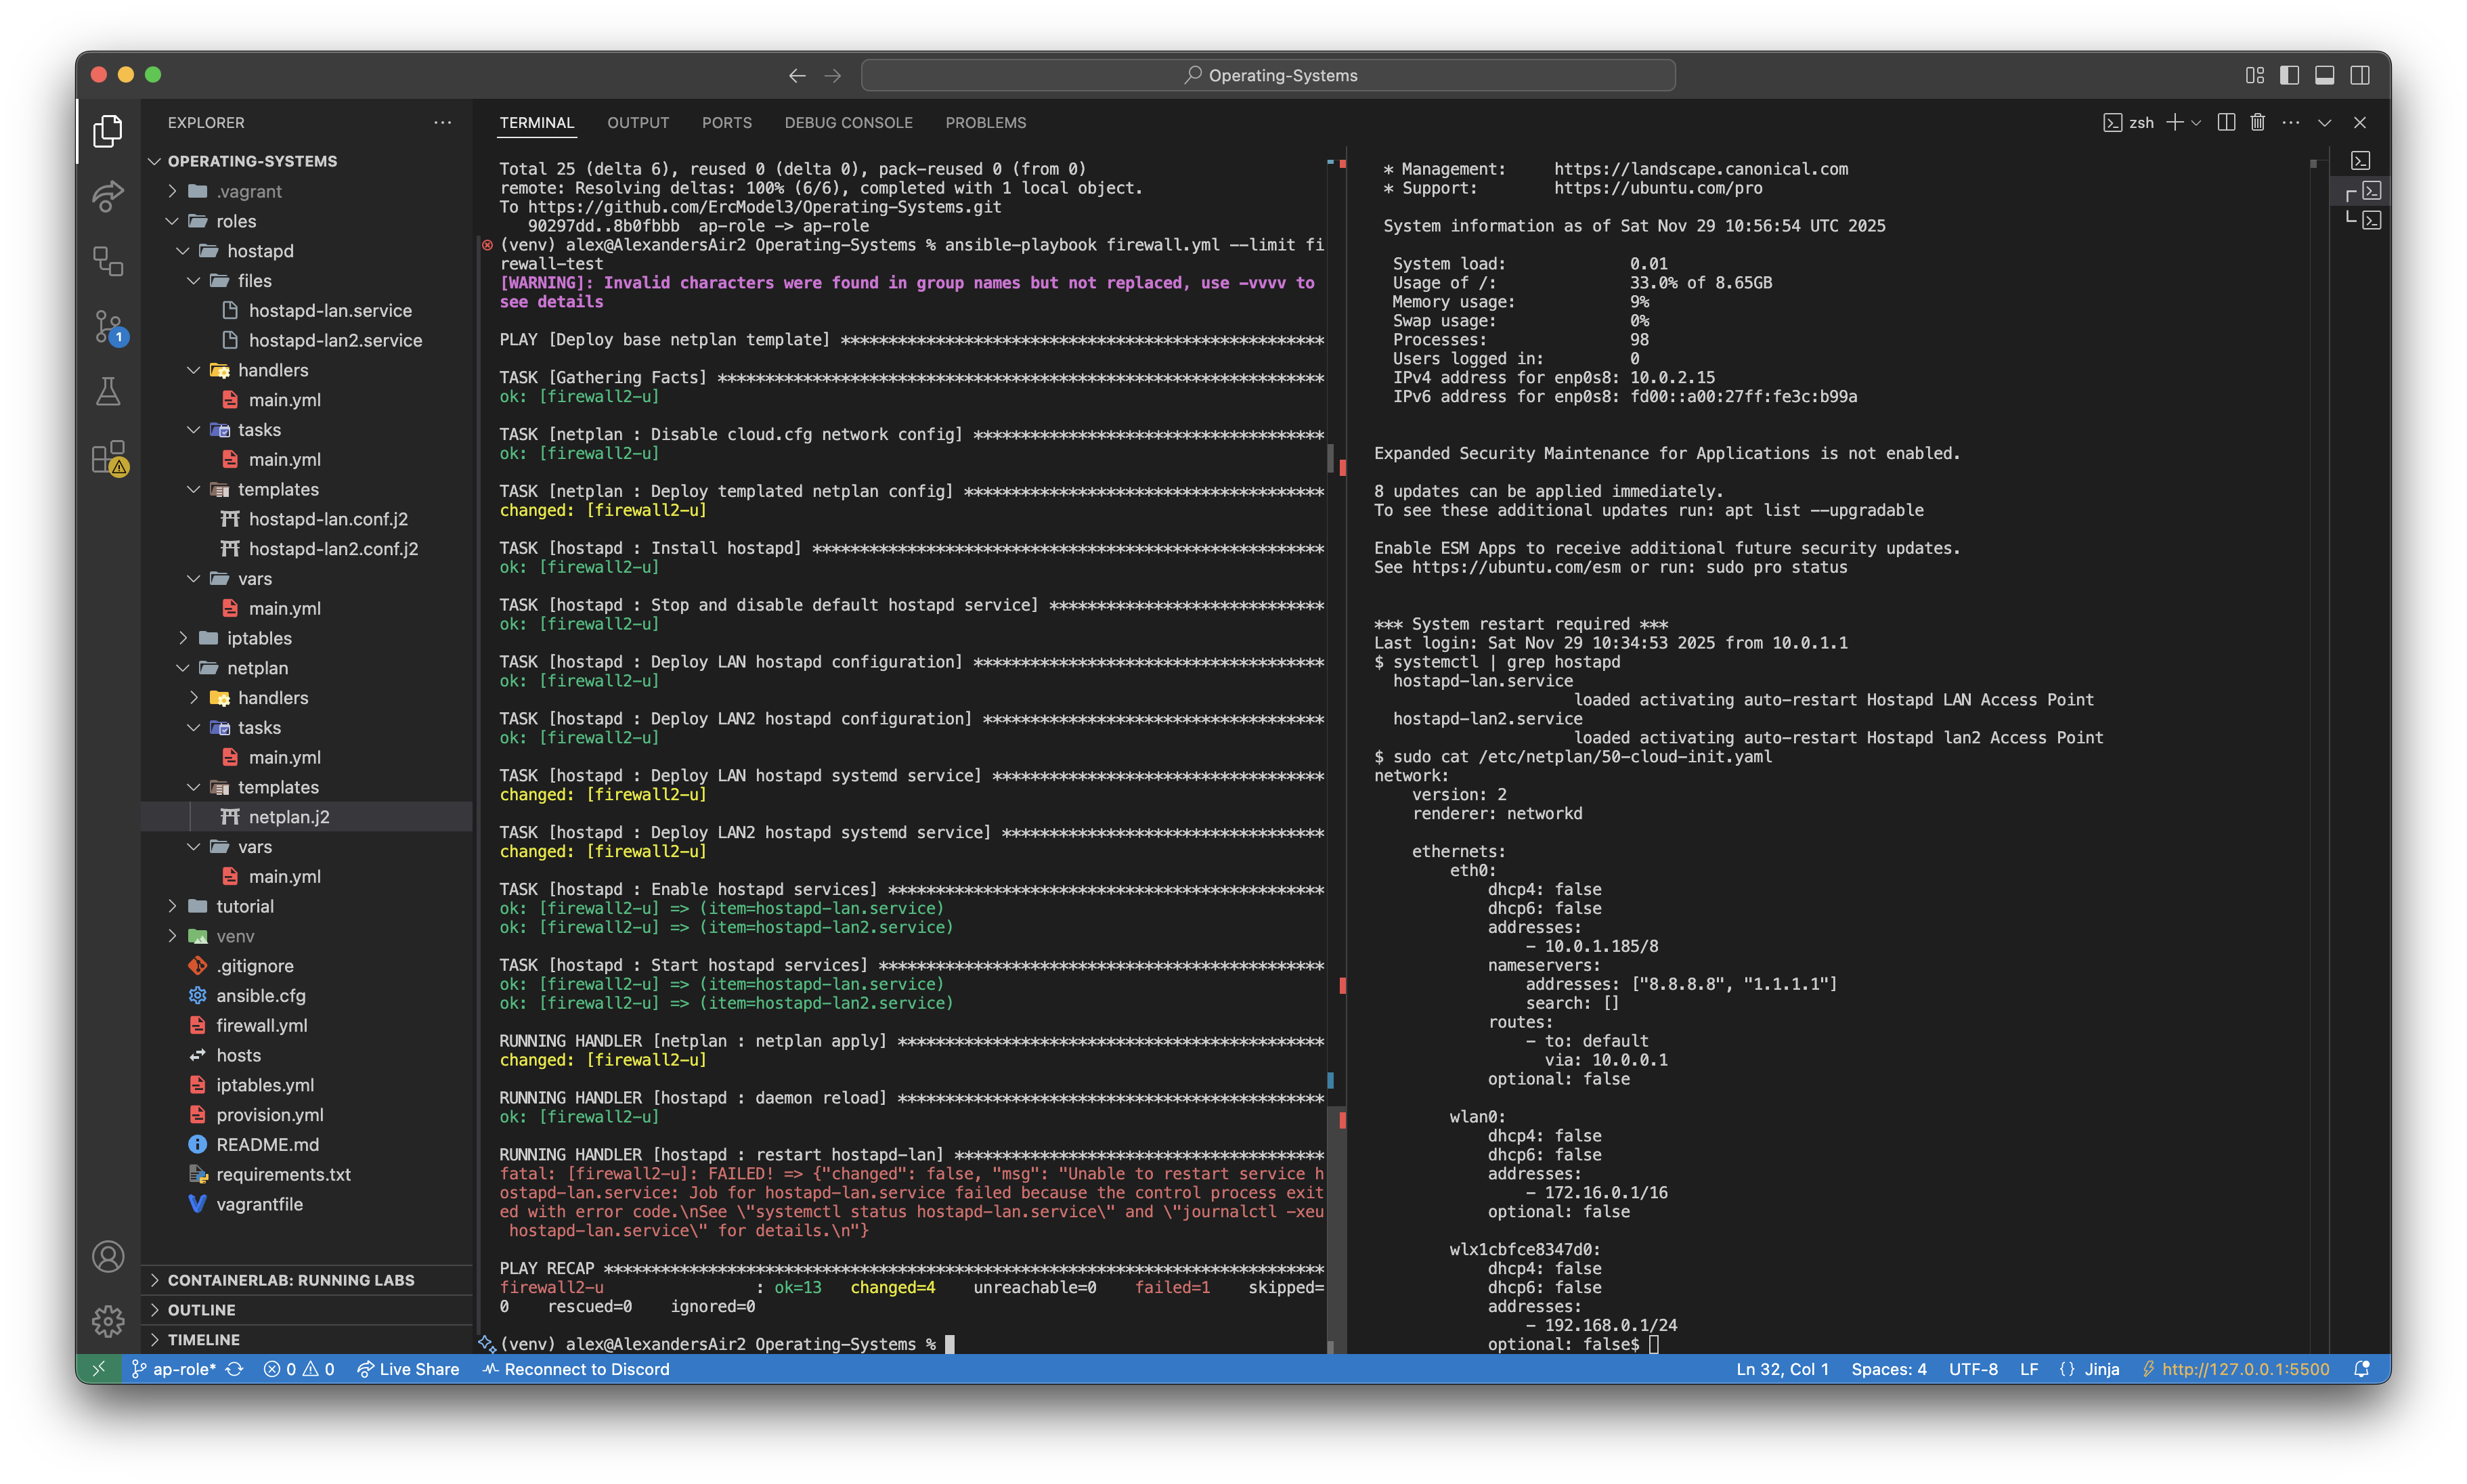
\includegraphics[width=1\linewidth]{Screenshots/image.png}
    \caption{Enter Caption}
    \label{fig:ansible-hostapd+netplan-deploy-prod}
\end{figure}

\begin{figure}[H]
    \centering
    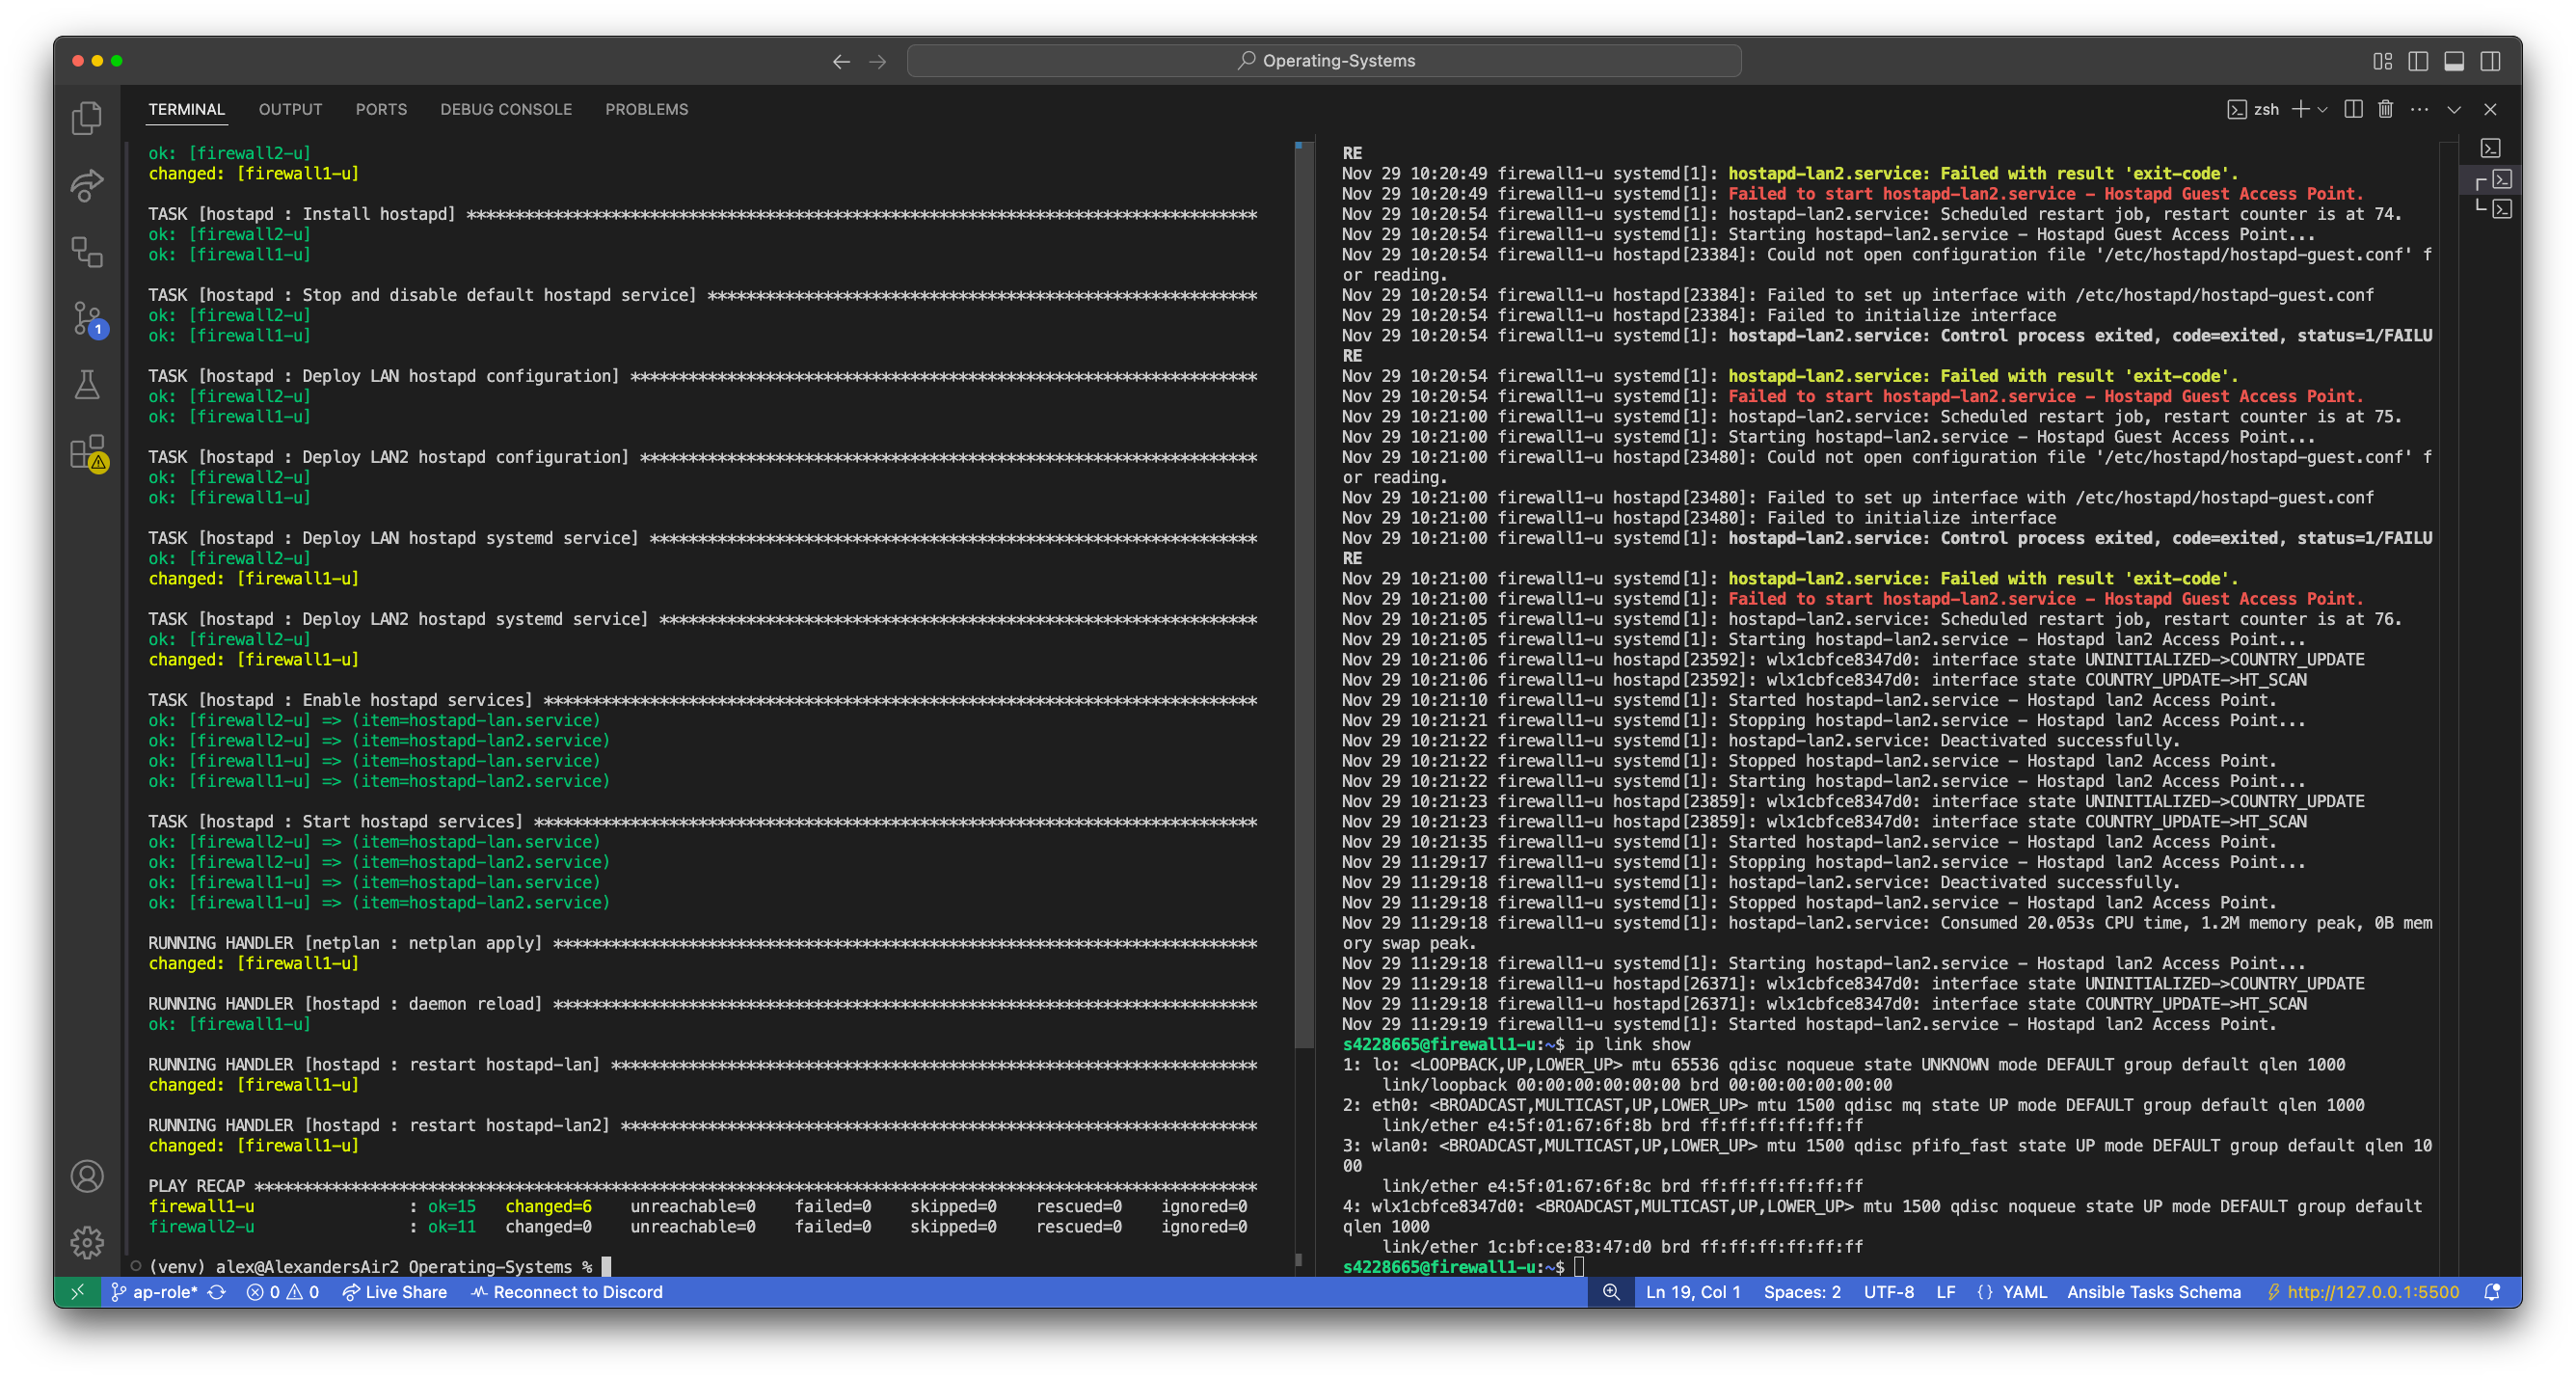
\includegraphics[width=1\linewidth]{Screenshots/vscode-both-firewall-deploy1.png}
    \caption{A successful firewall deployment on the LAN interface, but the LAN2 interface is still down}
    \label{fig:ansible-firewall-deploy1}
\end{figure}

After doing some troubleshooting (checking logs in figure \ref{fig:ansible-firewall-deploy1}) and seeing my own 2.4Ghz wifi go down, it looks like 

ISSUES









% Demo

The template uses Jinja2 variable substitution to separate configuration data from structure, enabling environment-specific deployments (testing vs. production) without modifying the template itself. Variables are defined in \texttt{roles/netplan/vars/main.yml} (Figure \ref{fig:netplan-vars}).

The WAN interface (\texttt{eth0}) is the only interface with a default route, ensuring all internet-bound traffic exits through the upstream gateway at \texttt{10.0.0.1}. The LAN and LAN2 interfaces (\texttt{eth1}, \texttt{eth2}) do not define routes, as the firewall itself is the gateway for these networks - routing decisions are handled by the iptables forwarding rules discussed in Section \ref{subsec:firewall-rules}.

DNS servers are configured only on the WAN interface using Google DNS (\texttt{8.8.8.8}) and Cloudflare DNS (\texttt{1.1.1.1}) as public resolvers. Internal zone devices receive DNS configuration via DHCP, which will be discussed in the DHCP server configuration (if implemented) or rely on the firewall to forward DNS queries.

\subsubsection{Configuration Verification}
\label{subsubsec:netplan-verify}

After Ansible deployment, the netplan configuration can be verified using the \texttt{ip addr} command to confirm all three interfaces have received their static IP addresses:

\begin{verbatim}
ubuntu@raspberrypi:~$ ip addr show
2: eth0: <BROADCAST,MULTICAST,UP,LOWER_UP> mtu 1500
    inet 10.0.0.2/8 brd 10.255.255.255 scope global eth0
3: eth1: <BROADCAST,MULTICAST,UP,LOWER_UP> mtu 1500
    inet 172.16.0.1/16 brd 172.16.255.255 scope global eth1
4: eth2: <BROADCAST,MULTICAST,UP,LOWER_UP> mtu 1500
    inet 192.168.0.1/24 brd 192.168.255.255 scope global eth2
\end{verbatim}

The \texttt{ip route} command confirms that the default route points to the WAN gateway, with directly connected routes for LAN and Guest subnets:

\begin{verbatim}
ubuntu@raspberrypi:~$ ip route show
default via 10.0.0.1 dev eth0 proto static
10.0.0.0/8 dev eth0 proto kernel scope link src 10.0.0.2
172.16.0.0/16 dev eth1 proto kernel scope link src 172.16.0.1
192.168.0.0/24 dev eth2 proto kernel scope link src 192.168.0.1
\end{verbatim}

% \subsection{Firewall Rules Implementation}
\label{subsec:firewall-rules}
% Document all required rules with explanations

\subsubsection{Class A config}
% Implementation details

\subsubsection{Class B config}
% Implementation details

\subsubsection{Class C config}
% Implementation details

\subsubsection{Essential Services Configuration}
% DNS, DHCP, ICMP rules

\subsubsection{Packet Forwarding Rules}
% NAT and forwarding configuration

\subsubsection{Access Control Rules}
% SSH/RDP restrictions, VNC blocking

\section{Resource Monitoring}
\label{sec:resource-monitoring}
% 400-500 words total

\subsection{Monitoring Tools Setup}
\label{subsec:monitoring-tools}
% Tools selection and justification, installation and configuration

\subsection{Key Performance Indicators}
\label{subsec:kpi}
% CPU utilisation, memory usage, network throughput, packet processing rates,
% temperature monitoring

\subsection{Data Collection Methodology}
\label{subsec:data-collection}
% Benchmarking approach, monitoring duration, data visualisation tools

%----------------------------------------------------------------------------------------
%	PERFORMANCE EVALUATION AND SCALABILITY
%----------------------------------------------------------------------------------------
\section{Performance Evaluation and Scalability}
\label{sec:performance}
% 600-800 words total

\subsection{Testing Scenarios}
\label{subsec:testing-scenarios}
% Document different test cases

\subsubsection{Normal Traffic Conditions}
% Test details and results

\subsubsection{High Load Testing}
% Stress test methodology and results

\subsubsection{Security Testing}
% DDoS simulation, penetration attempts

\subsection{Performance Metrics}
\label{subsec:metrics}
% Latency measurements, throughput analysis, packet loss rates, connection limits

\subsection{Results Analysis}
\label{subsec:results}
% Performance graphs and charts, comparative analysis, bottleneck identification

% Example for including performance graphs:
% \begin{figure}[H]
% \centering
% \includegraphics[width=0.7\textwidth]{cpu_usage_graph.png}
% \caption{CPU Usage Under Different Load Conditions}
% \label{fig:cpu-usage}
% \end{figure}

\subsection{System Scalability}
\label{subsec:scalability}
% Maximum capacity assessment, limitations and constraints, optimization recommendations

%----------------------------------------------------------------------------------------
%	TESTING AND VALIDATION
%----------------------------------------------------------------------------------------
\section{Testing and Validation}
\label{sec:testing}
% 300-400 words
% Firewall rule testing methodology, security validation tests,
% traffic flow verification, screenshot evidence

%----------------------------------------------------------------------------------------
%	CONCLUSION AND RECOMMENDATIONS
%----------------------------------------------------------------------------------------
\section{Conclusion and Recommendations}
\label{sec:conclusion}
% 300-400 words
% Project achievements summary, key findings, system limitations,
% future improvements, recommendations for production use

%----------------------------------------------------------------------------------------
%	REFERENCES (Harvard Style)
%----------------------------------------------------------------------------------------
\newpage
% \bibliographystyle{agsm} % Harvard style
% \begin{thebibliography}{99}


% \appendix
\section{Ansible}
\label{app:Ansible}
\subsubsection{ansible.cfg}
\label{subsec:ansible}
\begin{minted}{YAML}
Balls
\end{minted}


\section{Ansible Roles}
\label{app:Ansible-roles}

\subsection{iptables.yml}
\subsubsection{tasks/main.yml}
\begin{minted}{YAML}
Balls
\end{minted}

\subsubsection{templates/class-a.j2}
\begin{minted}{Python}
Class A
\end{minted}

\subsubsection{templates/class-b.j2}
\begin{minted}{Python}
Class B
\end{minted}

\subsubsection{templates/class-c.j2}
\begin{minted}{Python}
Class C
\end{minted}


\section{Firewall Configuration Files}
\label{app:config}
% Include complete configuration files

\section{Firewall Rulesets}
\label{app:rules}

\subsection{Class-A Network Rules (WAN)}
\label{subsec:class-a-rules}

The Class-A network rules apply to the WAN interface (eth0) connecting to the external internet. These rules implement strict ingress filtering, allow essential services, enable packet forwarding to internal networks, and include anti-spoofing measures.

\begin{verbatim}
*filter
:INPUT DROP [0:0]
:FORWARD DROP [0:0]
:OUTPUT ACCEPT [0:0]

-A INPUT -i lo -j ACCEPT
-A INPUT -m state --state ESTABLISHED,RELATED -j ACCEPT

-A INPUT -p tcp --dport 22 -m state --state NEW -j ACCEPT
-A INPUT -i eth0 -p icmp --icmp-type echo-request -j ACCEPT

-A INPUT -i eth0 -p tcp --dport 80 -j ACCEPT
-A INPUT -i eth0 -p tcp --dport 443 -j ACCEPT

-A INPUT -i eth0 -p udp --dport 53 -j ACCEPT
-A INPUT -i eth0 -p tcp --dport 53 -j ACCEPT

-A INPUT -j LOG --log-prefix "INPUT-DROP: " --log-level 4
-A INPUT -j DROP

-A FORWARD -m state --state ESTABLISHED,RELATED -j ACCEPT

-A FORWARD -i eth1 -o eth0 -j ACCEPT
-A FORWARD -i eth2 -o eth0 -j ACCEPT

-A FORWARD -i eth1 -o eth2 -j DROP
-A FORWARD -i eth2 -o eth1 -j DROP

-A FORWARD -p tcp --dport 22 -j DROP
-A FORWARD -p tcp --dport 23 -j DROP
-A FORWARD -p tcp --dport 3389 -j DROP

-A FORWARD -p tcp --tcp-flags ALL NONE -j DROP
-A FORWARD -p tcp --tcp-flags ALL ALL -j DROP

-A FORWARD -j LOG --log-prefix "FORWARD-DROP: " --log-level 4
-A FORWARD -j DROP

COMMIT

*nat
:PREROUTING ACCEPT [0:0]
:INPUT ACCEPT [0:0]
:OUTPUT ACCEPT [0:0]
:POSTROUTING ACCEPT [0:0]

-A POSTROUTING -o eth0 -j MASQUERADE

-A POSTROUTING -s 172.16.0.0/16 -o eth0 -j MASQUERADE
-A POSTROUTING -s 192.168.0.0/24 -o eth0 -j MASQUERADE

COMMIT

*mangle
:PREROUTING ACCEPT [0:0]
:INPUT ACCEPT [0:0]
:FORWARD ACCEPT [0:0]
:OUTPUT ACCEPT [0:0]
:POSTROUTING ACCEPT [0:0]

-A PREROUTING -m conntrack --ctstate INVALID -j DROP

-A PREROUTING -p tcp ! --syn -m conntrack --ctstate NEW -j DROP

-A PREROUTING -p tcp --tcp-flags ALL NONE -j DROP
-A PREROUTING -p tcp --tcp-flags ALL ALL -j DROP
-A PREROUTING -p tcp --tcp-flags SYN,FIN SYN,FIN -j DROP
-A PREROUTING -p tcp --tcp-flags SYN,RST SYN,RST -j DROP

-A PREROUTING -f -j DROP

COMMIT
\end{verbatim}

\subsection{Class-B Network Rules (LAN)}
\label{subsec:class-b-rules}

The Class-B network rules apply to the LAN interface (eth1) serving the trusted network segment. These rules permit internal management traffic, DNS/DHCP services, and restrict forbidden protocols while maintaining isolation from LAN2.

\begin{verbatim}
*filter
:INPUT DROP [0:0]
:FORWARD DROP [0:0]
:OUTPUT ACCEPT [0:0]

-A INPUT -i lo -j ACCEPT
-A INPUT -m state --state ESTABLISHED,RELATED -j ACCEPT

-A INPUT -p tcp --dport 22 -m state --state NEW -j ACCEPT
-A INPUT -i eth1 -p icmp --icmp-type echo-request -j ACCEPT

-A INPUT -i eth1 -p udp --dport 67 -j ACCEPT
-A INPUT -i eth1 -p udp --dport 68 -j ACCEPT

-A INPUT -i eth1 -p udp --dport 53 -j ACCEPT
-A INPUT -i eth1 -p tcp --dport 53 -j ACCEPT

-A INPUT -i eth1 -p tcp --dport 80 -j ACCEPT
-A INPUT -i eth1 -p tcp --dport 443 -j ACCEPT

-A INPUT -i eth1 -p tcp --dport 3000 -j ACCEPT
-A INPUT -i eth1 -p tcp --dport 8080 -j ACCEPT

-A INPUT -s 172.16.0.0/16 -i eth1 -j ACCEPT

-A INPUT -j LOG --log-prefix "INPUT-DROP-LAN: " --log-level 4
-A INPUT -j DROP

-A FORWARD -m state --state ESTABLISHED,RELATED -j ACCEPT

-A FORWARD -i eth1 -o eth0 -s 172.16.0.0/16 -j ACCEPT

-A FORWARD -i eth1 -o eth2 -j DROP

-A FORWARD -i eth0 -o eth1 -d 172.16.0.0/16 -m state --state ESTABLISHED,RELATED -j ACCEPT

-A FORWARD -p tcp --dport 25 -j DROP
-A FORWARD -p tcp --dport 135 -j DROP
-A FORWARD -p tcp --dport 139 -j DROP
-A FORWARD -p tcp --dport 445 -j DROP

-A FORWARD -j LOG --log-prefix "FORWARD-DROP-LAN: " --log-level 4
-A FORWARD -j DROP

COMMIT

*nat
:PREROUTING ACCEPT [0:0]
:INPUT ACCEPT [0:0]
:OUTPUT ACCEPT [0:0]
:POSTROUTING ACCEPT [0:0]

-A POSTROUTING -s 172.16.0.0/16 -o eth0 -j MASQUERADE

COMMIT

*mangle
:PREROUTING ACCEPT [0:0]
:INPUT ACCEPT [0:0]
:FORWARD ACCEPT [0:0]
:OUTPUT ACCEPT [0:0]
:POSTROUTING ACCEPT [0:0]

-A PREROUTING -i eth1 -m conntrack --ctstate INVALID -j DROP

-A PREROUTING -i eth1 -p tcp ! --syn -m conntrack --ctstate NEW -j DROP

-A PREROUTING -i eth1 -s 172.16.0.0/16 -j ACCEPT

COMMIT
\end{verbatim}

\subsection{Class-C Network Rules (LAN2)}
\label{subsec:class-c-rules}

The Class-C network rules apply to the LAN2 interface (eth2) serving untrusted devices. These rules implement the strictest filtering with rate limiting, block access to internal networks, restrict dangerous services (SSH, RDP, database ports), and implement anti-spoofing measures to prevent devices claiming RFC1918 addresses.

\begin{verbatim}
*filter
:INPUT DROP [0:0]
:FORWARD DROP [0:0]
:OUTPUT ACCEPT [0:0]

-A INPUT -i lo -j ACCEPT
-A INPUT -m state --state ESTABLISHED,RELATED -j ACCEPT

-A INPUT -i eth2 -p icmp --icmp-type echo-request -j ACCEPT

-A INPUT -i eth2 -p udp --dport 67 -j ACCEPT
-A INPUT -i eth2 -p udp --dport 68 -j ACCEPT

-A INPUT -i eth2 -p udp --dport 53 -j ACCEPT
-A INPUT -i eth2 -p tcp --dport 53 -j ACCEPT

-A INPUT -i eth2 -p tcp --dport 80 -j ACCEPT
-A INPUT -i eth2 -p tcp --dport 443 -j ACCEPT

-A INPUT -i eth2 -p tcp --dport 22 -m state --state NEW -j ACCEPT

-A INPUT -i eth2 -s 192.168.0.0/24 -m limit --limit 10/min -j ACCEPT

-A INPUT -j LOG --log-prefix "INPUT-DROP-GUEST: " --log-level 4
-A INPUT -j DROP

-A FORWARD -m state --state ESTABLISHED,RELATED -j ACCEPT

-A FORWARD -i eth2 -o eth0 -s 192.168.0.0/24 -j ACCEPT

-A FORWARD -i eth2 -o eth1 -j DROP

-A FORWARD -i eth2 -d 172.16.0.0/16 -j DROP

-A FORWARD -i eth0 -o eth2 -d 192.168.0.0/24 -m state --state ESTABLISHED,RELATED -j ACCEPT

-A FORWARD -i eth2 -p tcp --dport 22 -j DROP
-A FORWARD -i eth2 -p tcp --dport 23 -j DROP
-A FORWARD -i eth2 -p tcp --dport 3389 -j DROP

-A FORWARD -i eth2 -p tcp --dport 135 -j DROP
-A FORWARD -i eth2 -p tcp --dport 139 -j DROP
-A FORWARD -i eth2 -p tcp --dport 445 -j DROP

-A FORWARD -i eth2 -p tcp --dport 1433 -j DROP
-A FORWARD -i eth2 -p tcp --dport 3306 -j DROP
-A FORWARD -i eth2 -p tcp --dport 5432 -j DROP

-A FORWARD -i eth2 -m limit --limit 100/sec --limit-burst 200 -j ACCEPT

-A FORWARD -j LOG --log-prefix "FORWARD-DROP-GUEST: " --log-level 4
-A FORWARD -j DROP

COMMIT

*nat
:PREROUTING ACCEPT [0:0]
:INPUT ACCEPT [0:0]
:OUTPUT ACCEPT [0:0]
:POSTROUTING ACCEPT [0:0]

-A POSTROUTING -s 192.168.0.0/24 -o eth0 -j MASQUERADE

COMMIT

*mangle
:PREROUTING ACCEPT [0:0]
:INPUT ACCEPT [0:0]
:FORWARD ACCEPT [0:0]
:OUTPUT ACCEPT [0:0]
:POSTROUTING ACCEPT [0:0]

-A PREROUTING -i eth2 -m conntrack --ctstate INVALID -j DROP

-A PREROUTING -i eth2 -p tcp ! --syn -m conntrack --ctstate NEW -j DROP

-A PREROUTING -i eth2 -p tcp --tcp-flags ALL NONE -j DROP
-A PREROUTING -i eth2 -p tcp --tcp-flags ALL ALL -j DROP
-A PREROUTING -i eth2 -p tcp --tcp-flags SYN,FIN SYN,FIN -j DROP
-A PREROUTING -i eth2 -p tcp --tcp-flags SYN,RST SYN,RST -j DROP

-A PREROUTING -i eth2 -s 192.168.0.0/24 -j ACCEPT

-A PREROUTING -i eth2 -s 10.0.0.0/8 -j DROP
-A PREROUTING -i eth2 -s 172.16.0.0/12 -j DROP

COMMIT
\end{verbatim}

\section{Testing Scripts}
\label{app:scripts}
% Network testing and monitoring scripts

\section{Additional Screenshots}
\label{app:screenshots}
% Supporting visual evidence

\section{Command Outputs}
\label{app:outputs}
% Full command execution results

\newpage
\printbibliography
\end{document}

balls balls balls